\documentclass[a4paper,10pt,titlepage]{report}

\usepackage{xspace}
\usepackage{xargs}  
\usepackage[pdftex,dvipsnames]{xcolor}

\usepackage[font=bf,]{caption}
\usepackage{subcaption}
\input{glyphtounicode}

\usepackage{lastpage}

\usepackage[english]{babel}
\usepackage[utf8]{inputenc}
\usepackage{csquotes}
\usepackage[margin=1in]{geometry}
\usepackage{fancyhdr}
\usepackage{booktabs}
\usepackage{paralist}
\usepackage{graphicx}
\usepackage{tabularx}
\usepackage{adjustbox}
\usepackage{titlepic}
\usepackage{vhistory}
\usepackage{enumitem}
\usepackage{longtable}
\usepackage[backend=biber, style=ieee,citestyle=numeric-comp]{biblatex}
\usepackage[colorinlistoftodos, prependcaption]{todonotes}
\usepackage{placeins}
\usepackage{multirow}
\usepackage{amsmath}
\usepackage[hidelinks]{hyperref}
\usepackage[acronym,nogroupskip,nohypertypes={acronym},toc,section=chapter]{glossaries}
\usepackage{amssymb}
\usepackage{verbatim}
\usepackage{cmap}

\input{glyphtounicode}

\pdfglyphtounicode{f_f}{FB00}
\pdfglyphtounicode{f_f_i}{FB03}
\pdfglyphtounicode{f_f_l}{FB04}
\pdfglyphtounicode{f_i}{FB01}

\pdfgentounicode=1

\usepackage[titletoc]{appendix}
\usepackage{tcolorbox}
\usepackage{listings}

% MY STUFF
\usepackage{float}
\usepackage{epigraph}
\usepackage{colortbl}
\usepackage{lscape} 
\usepackage{pifont}
\usepackage{array}
\usepackage{fixltx2e}
\usepackage{subcaption}
\usepackage{mwe}
\usepackage{fourier}
\usepackage[scaled=0.75]{FiraMono}

\DeclareUnicodeCharacter{0301}{\'{e}}

\newcommand{\cmark}{\ding{51}}
\newcommand{\xmark}{\ding{55}}

\lstset{morekeywords={},showstringspaces=false,basicstyle=\ttfamily,keywordstyle=\bfseries}

\definecolor{commentGreen}{RGB}{128,127,41}
\definecolor{stringGreen}{RGB}{0,127,38}
\definecolor{keywordRed}{RGB}{151,0,11}
\definecolor{typePurple}{RGB}{128,3,82}
\definecolor{variableBlue}{RGB}{0,0,255}
\definecolor{annotationRed}{RGB}{198,4,38}
\definecolor{annotationBlue}{RGB}{32,21,223}

\lstdefinelanguage[drl]{Drools}{
    sensitive=true,
    keywordsprefix=\$,
    alsoletter={:, },
    morekeywords=[2]{long,int,boolean,double,float,enum},
    morekeywords=[3]{package,import,declare,end,extends,from,insert,modify,not,new,no loop,query,retract,rule,salience,then,this,when, eval},
    morekeywords=[4]{after,before,during,over window:length,over window:time,overlaps},
    morekeywords=[5]{{no loop},over window:length,over window:time},
    morecomment=[l]{//},
    morecomment=[s]{/*}{*/},
    moredelim=[s][\color{annotationRed}\itshape]{@}{)},
    moredelim=[s][\color{annotationBlue}\itshape]{@[}{]},
    morestring=[b]",
    morestring=[d]',
%%% default style
    basicstyle=\footnotesize\ttfamily,
    numbers=left,
    stepnumber=1,
    showstringspaces=false,
    tabsize=1,
    breaklines=true,
    breakatwhitespace=false,
    commentstyle=\color{commentGreen}\itshape,
    keywordstyle=\color{keywordRed}\bfseries,
    keywordstyle=[1]\color{variableBlue}\itshape,
    keywordstyle=[2]\color{typePurple}\bfseries,
    keywordstyle=[3]\color{keywordRed}\bfseries,
    keywordstyle=[4]\color{keywordRed}\bfseries,
    keywordstyle=[5]\color{stringGreen}\bfseries,
    stringstyle=\color{stringGreen}
}[comments,keywords,strings]

%

\newcommand{\ie}{\emph{i.e.},\xspace}
\newcommand{\eg}{\emph{e.g.},\xspace}
\newcommand{\etc}{\emph{etc.}\xspace}
\newcommand{\etal}{\emph{et al.}\xspace}

\newcommand{\sig}{\gls{sig}}
\newcommand{\sigs}{\glspl{sig}}

\newcommandx{\unsure}[2][1=]{\todo[linecolor=red,backgroundcolor=red!25,bordercolor=red,#1, inline]{#2}}
\newcommandx{\discussion}[2][1=]{\todo[linecolor=red,backgroundcolor=green!25,bordercolor=red,inline,#1]{#2}}

\newcommandx{\improvement}[2][1=]{\todo[linecolor=blue,backgroundcolor=blue!25,bordercolor=blue,#1]{#2}}

\newcommandx{\reminder}[2][1=]{\todo[linecolor=yellow,backgroundcolor=yellow!25,bordercolor=yellow,#1]{#2}}

\newcommandx{\lessprio}[2][1=]{\todo[linecolor=Plum,backgroundcolor=Plum!25,bordercolor=Plum,#1]{#2}}
\newcommandx{\todocontent}[2][1=]{\todo[author=\textbf{Planned content},backgroundcolor=Goldenrod!25,bordercolor=Goldenrod,inline,#1]{#2}}


\newcolumntype{L}[1]{>{\raggedright\let\newline\\\arraybackslash\hspace{0pt}}p{#1}}
\newcolumntype{C}[1]{>{\centering\let\newline\\\arraybackslash\hspace{0pt}}p{#1}}
\newcolumntype{R}[1]{>{\raggedleft\let\newline\\\arraybackslash\hspace{0pt}}p{#1}}

\definecolor{ryel}{HTML}{fcd116}
\definecolor{rred}{HTML}{ce1126}
\definecolor{rblu}{HTML}{0a3eb9}

\newcommand{\email}[1]{\ttfamily\href{mailto:#1}{#1}}

\newcommand{\uvacoverfoot}{%
	\vfill
	\begin{center}
		\begin{tabular}{r|l}
			\multirow{3}{*}{
\includegraphics[height=48pt]{uva.pdf}}
			&\textsc{\Large Universiteit van Amsterdam}\\
			&\textsc{Faculteit der Natuurwetenschappen, Wiskunde en Informatica}\\
			&\textsc{Master Software Engineering}\\
			&\url{http://www.software-engineering-amsterdam.nl}
		\end{tabular}
	\end{center}
}

\renewcommand{\maketitle}{
	\thispagestyle{empty}
	\enlargethispage{30pt}
	\renewcommand{\thefootnote}{\fnsymbol{footnote}}
	\setcounter{page}{0}
	\vspace{60pt}
	\begin{center}
		{\Huge\bfseries Projecting Rules: Improving Comprehension of Business Rules with Projectional Editing \par}
		
		\vspace{44pt}
		{\Large\bfseries Paul \textsc{Spencer} \par}
		\email{paul.spencer@student.uva.nl}\\
		\vspace{11pt}
		November 30, 2021, \pageref{LastPage} pages
	\end{center}
	\vfill
	\begin{tabular}{ll}
		\textbf{Academic supervisor:} 	& Dr. Clemens \textsc{Grelck}, \email{c.grelck@uva.nl} \\
		\textbf{Daily supervisor:} & Toine \textsc{Khonraad}\\
		\textbf{Host organisation:} & Khonraad / Visma, \url{https://www.visma.com/}
	\end{tabular}
	\uvacoverfoot
	\newpage
	\setcounter{footnote}{0}
	\renewcommand{\thefootnote}{\arabic{footnote}}
	\setlength{\parskip}{0pt}
}
  
\pagestyle{fancy}
\fancyhf{}
\fancyhead[L]{\leftmark}
\fancyfoot[C]{\thepage}
\setlength{\headheight}{14pt}


\newcounter{findingctr}

\newenvironment{finding}{
	\refstepcounter{findingctr}
	\begin{tcolorbox}
	\textbf{Finding \thefindingctr:}
}{\end{tcolorbox}} 

\setlist{noitemsep,topsep=4pt,parsep=1pt,partopsep=4pt}


\lstset{
	basicstyle=\footnotesize,
	breakatwhitespace=false,
	breaklines=true,
	captionpos=b,
	frame=single,
	language=Java,
	keywordstyle=\bf,
	tabsize=2
}

\setlength\extrarowheight{2pt}

\bibliography{main}

\begin{document}
    \maketitle
    \begin{abstract}
\addchaptertocentry{\abstractname} 

\noindent
\textit{Context}: 
Declarative rules engine languages, such as Drools, can become difficult to reason about when there are many rules.

\noindent
\textit{Objective}: 
This project investigates whether projectional editing is a valid solution to this issue.
If so, how can different projections of the code can ease the comprehensibility of the code.

\noindent
\textit{Method}: 
We conducted a systematic literature review, to ascertain the relevancy of projectional editing.
We created an implementation of the Drools language using the MPS language workbench and made innovative projections of Drools ASTs.
We validated our projections with a survey.

\noindent
\textit{Results}:
Projectional editing is still niche, though it is making some industrial and educational headway in particular with JetBrains MPS.
Projections can be useful, though, our survey found that our projections did not outperform the understanding of textual representation at least amongst experience Drools users.

\noindent
\textit{Keywords}:
projectional editing; Rules Engines; MPS; Drools

\noindent
\textit{Paper type}:
Research paper
\end{abstract}

    \tableofcontents
    \chapter{Introduction}
\label{chapter:Introduction}

\epigraph{The limits of my language mean the limits of my world.}{\textit{Logico-Tractatus Philosophicus\\Ludwig Wittgenstein}}

\section{Problem statement}

Miller's Law\cite{miller1956magical} states that an average human can hold in his short-term memory 5-9 objects.
This is often an argument for more succinct code.  
The argument being anything that is not immediately in the developers vision has to be stored in her memory.
With it being impractical to reason about code that she cannot recall, then the fewer relevant items to her reasoning that are out of view the easier it is to reason about the code.

[TODO: complete the problem statement]



\subsection{Research questions}

The research question we wish to answer is:
\begin{itemize}
    \item \textbf{Main research question:} ``How can projectional editors and DSLs be combined to address feedback mechanisms for developers in the context of reasoning about rules in a rule-based business engine?''
\end{itemize}

This question requires knowing if it is possible with current tooling, thus we would like to answer the question:
\begin{itemize}
    \item \textbf{RQ 1:} ``What is the current state of language workbenches supporting projectional editing?''
\end{itemize}

Finally, we specifically would like to know how we can improve the ability to reason about the business rules engine, so we ask the question:
\begin{itemize}
    \item \textbf{RQ 2:} ``Which projections can help developers to get appropriate feedback about rules?''
\end{itemize}



\section{Contributions}

This thesis proposes a representation of business rules in a concise and readable format that could solve comprehensibility issues resulting from large code-bases of business rules.
The implementation behind the approach relies on language engineering and projectional editing.
We developed a stand-alone opensource solution on a limited implementation of Drools.
The underlying Drools implementation can be used as a base language for model-to-model generation by the MPS ecosystem.

\section{Project context}

This investigation was hosted by Khonraad Software Engineering, a subsidiary of Visma.
Khonraad provides mission-critical services focussed on the automation of workflows at the cross-section of local government and healthcare.
Specifically, Khonraad facilitates the mental health care and coercion laws in the Netherlands - WVGGZ, WZD, and WTH - which provide agencies the ability to intervene in domestic violence, psychiatric disorders, and illnesses.

Khonraad's system facilitates reporting and communication between municipalities, police, judiciary, lawyers, mental health care, and many social care institutions.
The system has 15,000 users and is available 24/7.

Configuration and administration use complex matrices of compliance mechanisms, access user rights and communication settings.
The sensitivity of the personal data, being both medical and criminal, means security is of utmost importance.
The security against data loss, preventing unlawful disclosure and guaranteeing availability, especially during crisis situations, is crucial.
Demonstration of the correctness of the, often changing, configuration is a major concern in the company.

This work environment allows us to work on an existing project, where the tangible success will have an impact on the lives of those in critical need.
Khonraad has it's own implementations in the Drools language, that have evolved over the iterations of the laws.
The evolution of the code base over the years means that the real-life issues we came across are not just thought experiments.

\section{Thesis Outline}

We start in chapter \ref{chapter:Background} with the required background information on rules engines and projectional editing.
In chapter \ref{chapter:SLR} we describe our efforts to answer our first research question using a systematic literature review.
Chapter \ref{chapter:ADR} describes the approaches and outcomes of answering the second research question using active design research. 
Chapter \ref{chapter:Survey} brings us to research question 3 and the survey we used to explore it.
We then investigate related work in chapter \ref{chapter:RelatedWork}.
Finally, we present the conclusions of our research in chapter \ref{chapter:Conclusion}.


    \chapter{Background}\label{chapter:Background}

This chapter gives the background information required on rules engines and projectional editing.
It presents the specific case of rules engine that we will be using for our investigation: Drools.
Further, it briefly examines the base tool type for creating Domain-specific languages: Language work benches.
Finally, it presents the specific projectional editing tool we will be using: JetBrains MPS.

\section{RulesEngines}

\subsection{What is a Rules Engine?}

In this section, we will describe what a rules engine is and a little of its history.

The Aristotelian doctrine of essentialism declares that a thing has essential properties and properties that are accidental.
If one takes away accidental properties, then the thing remains the thing.
If one takes away essential properties, the thing is no longer the thing.
If the thing is a business application, then its essential properties are its business rules.

Simply put, business rules are the principles or regulations by which an organization carries out the tasks needed to achieve its goals.
When adequately defined, it is possible to encode these rules into statements that define or constrain some business organizational behaviour.
A rule consists of a condition and an action.
When the condition is satisfied, then the action is performed.
More formally, business rules are the implication in the logical principle of Modus Ponens.

When described like this, one could imagine this as just the ``if-then'' logic frequently used in traditional programming.
One would not be wrong. 
However, in traditional programming, representing all the combinatorial outcomes can become complex.
In the typical application architecture, developers tend to distribute rules throughout the source code or database.
Each additional rule leads to more fragility.

We find descriptions of these rules in the design documentation or user manuals.
However, as applications evolve, documentation gets out of sync with the codebase.
Once desynchronization occurs, to know the rules governing the application, one has to navigate the codebase and decode the rules from often scattered locations.

A rules engine is also known as a Business Rules Engine, a Business Rules Management System or a Production Rules System.
The goal of a rules engine is to abstract business rules into encoded and packaged logic that defines the tasks of an organization with the accompanying tools that evaluate and execute these rules.
Simply put, they are where we evaluate our rules.
Rules engines match rules against facts and infer conclusions.
Returning to the Modus Ponens comparison:

\begin{tabular}{c@{\,}l@{}} 
    & $p$ \\
\arrayrulecolor{blue!60!green!70}    & $p \to q$ \\\cline{2-2}
$\therefore$         & $q$ \\
\end{tabular}

If the premise $p$ holds and the implication $p \to q$ holds, then the conclusion $q$ holds.
In terms of a rule engine and business rules, this would be:
\begin{enumerate}
    \setlength\itemsep{0em}
    \item the rules engine gathers the data for the premise: $p$
    \item it examines the business rules as the implications: $p \to q$
    \item it executes the conclusion: $q$
\end{enumerate}

Rules engines follow the recognize-act cycle.
First, the match, i.e. are there any rules with a true condition?
Next, they carry out conflict resolution, pick the most relevant matching rules.
They then perform the actions described in the rule.
Then back to the matching step.
If they make no more matches, they terminate the cycle.

Rules Engines are declarative, focussing on the what of the rules, not the how of the execution.
Date\cite{date2000not} describes a rules engine role as ``to specify business process declaratively, via business rules and get the system to compile those rules into the necessary procedural (and executable) code.''
Fowler\cite{Fowler_rulesEngine} describes a rules engine as follows: `` ... providing an alternative computational model.
Instead of the usual imperative model, which consists of commands in sequence with conditionals and loops, a rules engine is based on a Production Rule System.
This is a set of production rules, each of which has a condition and an action ...''.

Some of the advantages of using a rules engine include:
\begin{itemize}
    \setlength\itemsep{0em}
    \item The separation of knowledge from its implementation logic.
    \item The externalization of business logic.
    \item Rules can be human-readable.
\end{itemize}

In summary, a rules engine is the executor of a rules-based program, consisting of discreet declarative rules which model a part of the business domain.


Rule engines arose from the expert systems of the late 70s and early 80s.
Expert systems initially had three primary techniques for knowledge representation: Rules, frames and logic\cite{jackson1986introduction}.
``The granddaddy'' of the expert systems, MYCIN, relied heavily on rules-based knowledge representation\cite{shortliffe1974mycin} rather than long inference chains.
MYCIN was used to identify bacteria and recommend antibiotic prescriptions.
MYCIN and its progenitor, DENDRAL, spawned a whole family of Clinical Decision Support Systems that pushed the rules engine technology until the early 1980s.
Research into rules engines died out in the 1980s as it fell out of fashion.

Early in their existence, the rules engines hit a limiting factor because the matching algorithms they used suffered from the utility problem, i.e. the match cost increased linearly with the number of examined rules.
Charles Forgy's efficient pattern matching Rete algorithm\cite{forgy1989rete} and its successors solved this problem.
This algorithm works by modelling the rules as a network of nodes where each node type works as a filter.
A fact flows through the filters of this network.
The pre-calculation of this network is what provides the performance characteristics.

The first popular rules engine was Office Production System (OPS) from 1976.
In 1981 OPS5 added the Rete algorithm.
Currently, there are a few rules engines in use.
We show some of the more commonly used ones in table \ref{table:RuleEngines}.

\begin{table}
    \begin{center}
        \begin{tabular}{ |l c |l|l| } 
            \hline
            Product                      &                             & Developer    & licence type   \\
            \hline
            CLIPS                        &\cite{CLIPSProductPage}      & NASA         & open source    \\ 
            Drools                       &\cite{DroolsProductPage}     & JBoss/RedHat & open source    \\ 
            BizTalk Business Rule Engine &\cite{BiztalkProductPage}    & Microsoft    & proprietary    \\ 
            WebSphere ILOG JRules        &\cite{JRulesProductPage}     & IBM          & proprietary    \\ 
            OpenRules                    &\cite{OpenRulesProductPage}  & OpenRules    & open source    \\ 
            \hline
        \end{tabular}
    \end{center}
    \caption{Rules engine products}
    \label{table:RuleEngines}
\end{table}

\subsection{What is Drools?}\label{section:WhatIsDrools}

JBoss Rules, or more commonly known, Drools, is the leading opensource rules engine written in Java.
In this paper, when we use the name ``Drools'' we are referring to the ``Drools Expert'' which is the rule engine module of the Drools Suite.
Drools started in 2001 but rose to prominence with its 2005 2.0 release.
It is an advanced inference engine using an enhanced version of the Rete algorithm, called Rete\-OO\cite{sottara2010configurable}, adapted to an object-oriented interface specifically for Java.
Designed to accept pluggable language implementations, it can also work with Python and .Net.
It is considered one of the most developed and supported rules platforms.

To execute rules, Drools has four major components, as demonstrated in figure \ref{fig:Drools_components}.
The production memory contains the rules, and this will not change during an analysis session.
The rules are the focus of this thesis, and therefore, we will delve into much more detail later on these.

\begin{figure}[h]
    \centering
    \fbox{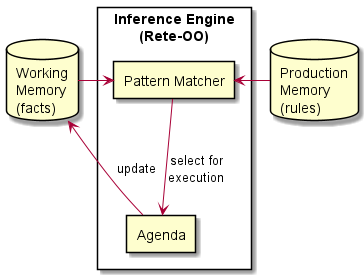
\includegraphics[width=0.55\textwidth]{Sections/images/components.png}}
    \caption{Drools components.}
    \label{fig:Drools_components}
\end{figure}

In Forgy's\cite{forgy1989rete} overview of a rete algorithm, the following steps occur.
\begin{enumerate}
    \item Match: Evaluate the LHSs of the productions to determine which are satisfied given the current contents of working memory.
    \item Conflict resolution: Select one production with a satisfied LHS; halt the interpreter if no productions have satisfied LHSs.
    \item Act: Perform the actions in the RHS of the selected production.
    \item Re-evaluate: Go To 1.
\end{enumerate}

Figure \ref{fig:Drools_inference_loop} show more detail of how these components interact within Drools to infer a conclusion.
First, Drools asserts facts in the working memory.
The working memory contains the current state of the facts, which triggers the inference engine.
Using the aforementioned Rete-OO algorithm, the pattern matcher will examine the working memory and a representation of the rules from the production memory to determine which rules are true.
Drools will then put the rules that match on the agenda.
It can be the case that many rules are concurrently true for the same fact assertion.
These rules conflict.
A conflict resolution strategy will decide which rule will fire in which order from the agenda.
The first rule on the agenda will fire.
If the rule modifies, retracts or asserts a fact, then the inference loop begins again.
We have inferred our conclusion if a rule specifies to halt or there are no matching rules left on the agenda.

\begin{figure}[h]
    \centering
    \fbox{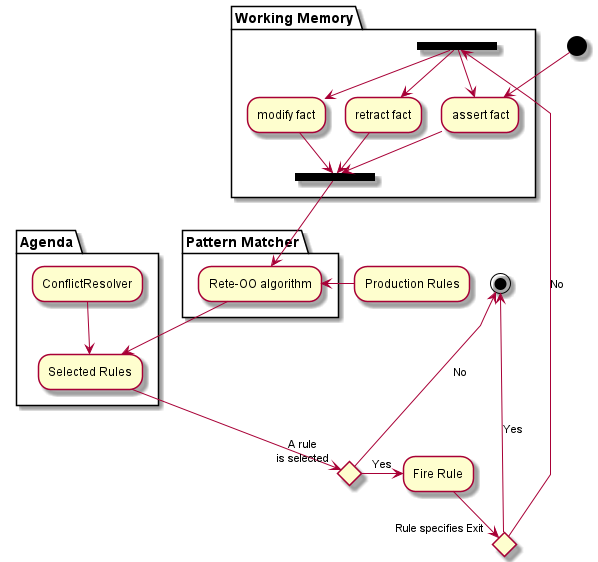
\includegraphics[width=0.55\textwidth]{Sections/images/InferenceLoop-1.png}}
    \caption{Drools inference loop}
    \label{fig:Drools_inference_loop}
\end{figure}

The component we will be focussing on in this paper is the rules.
A rules file containing the rules is a text file, typically with a .drl extension.
As the rules do not change during execution
During execution, the rules do not change, and Drools stores them in production memory.

We do not need to examine the rule file components package, import, global, declare, function and query.
We will examine the anatomy of a rule.

A rule consists of 3 parts: attributes, conditions, and consequences.
Attributes are optional hints to the inference engine as to how to examine a rule.
The conditional, ``when'', or left-hand side (LHS) of the rule statement is a block of conditions that have to, in aggregate, return true for the asserted fact. If true, then the rule is placed on the agenda.
The actions, consequences, ``then'', or right-hand side (RHS) of the rule statement contains actions to be executed when the rule is selected.

The LHS is a predicate statement made up of some patterns.
The patterns evaluate facts from the working memory.
The pattern can match against the existence of facts or facts with matching property conditions.
Connectives, such as not, and, and or can combine patterns.
The patterns apply to individual facts rather than the group, thus can be seen as first-order predicates.

Variables can be bound to facts that match these patterns for use later in the LHS or for updating the working memory on the RHS.

Drools offers more options for the LHS.
We have limited the scope of this paper to the features described thus far.

The RHS can contain arbitrary code that will execute when a rule is selected.
However, its primary purpose is to adjust the state of truth in the working memory.
One can insert, modify, and retract facts in the working memory.
Modifying and retracting facts must be done on fact variable references bound in the LHS.
One can explicitly terminate the inference loop with a halt command.

\begin{figure}[h]
    \centering
    \fbox{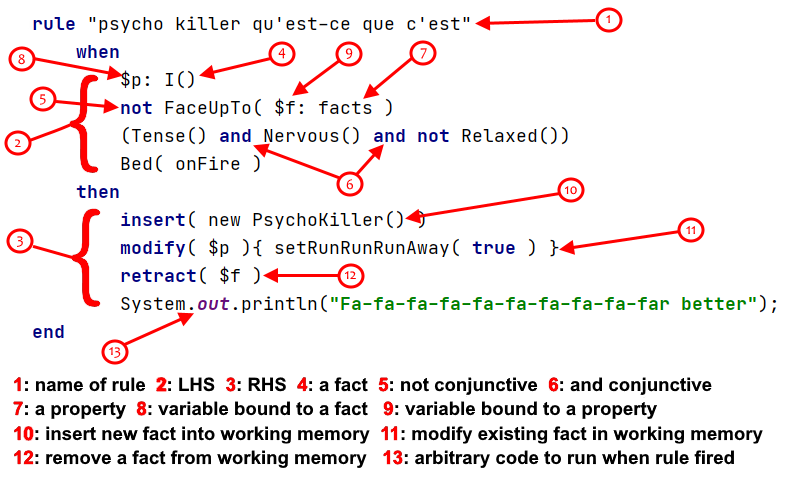
\includegraphics[width=0.95\textwidth]{Sections/images/DroolsRule2.png}}
    \caption{Drools rule breakdown}
    \label{fig:Drools_Rule_Breakdown}
\end{figure}

\subsubsection{An Explanatory Example}
Listing \ref{listing:drl_file} shows an example of a .drl file taken from the Drools sample code.

\noindent\begin{minipage}{\textwidth}
    \begin{lstlisting}[language={[drl]Drools}, caption=Example Drools file., captionpos=b, label=listing:drl_file]
        package org.drools.examples.honestpolitician
    
        import org.drools.examples.honestpolitician.Politician;
        import org.drools.examples.honest politician.Hope;
        
        rule ``We have an honest Politician''
            salience 10
            when
                exists( Politician( honest == true ) )
            then
                insertLogical( new Hope() );
        end
        
        rule ``Hope Lives''
            salience 10
            when
                exists( Hope() )
            then
                System.out.println(``Hurrah!!! Democracy Lives'');
        end
        
        rule ``Hope is Dead''
            when
                not( Hope() )
            then
                System.out.println( ``We are all Doomed!!! Democracy is Dead'' );
        end
        
        rule ``Corrupt the Honest''
            when
                $p : Politician( honest == true )   
                exists( Hope() )
            then
                System.out.println( ``I'm an evil corporation and I have corrupted `` + $p.getName() );
                modify( $p ) { 
                    setHonest( false ) 
                }
        end
    \end{lstlisting}
\end{minipage}

Listing \ref{listing:drl_file} gives the Drools engine instructions on what actions to take when something changes the working memory.
This toy example reacts to when the working memory has an honest politician added. 
It prints a message celebrating the existence of said politician.
It then corrupts her and gloats in a message.
Finally, it prints a message of despair.
The code in Listing \ref{listing:drl_file} does the following: 
\begin{enumerate}[topsep=2pt,itemsep=2pt,partopsep=2pt, parsep=2pt]
    \item On line 1, the package statement identifies the rule file.
    \item On lines 3 and 4, the import statements describe which facts are available for use.
    \item The ``We have an honest Politician'' rule on line 6 does the following:
    \begin{enumerate}[topsep=2pt,itemsep=2pt,partopsep=2pt, parsep=2pt]
        \item On line 7, using the salience attribute, the rule is set to be run before other rules with a lower salience.
        \item On line 10, the rule checks working memory for Politician facts with the honest property equal to true.
        \item On line 12, if found, then a Hope fact is inserted into the working memory.
    \end{enumerate}
    \item The ``Hope Lives'' rule on line 15 does the following:
    \begin{enumerate}[topsep=2pt,itemsep=2pt,partopsep=2pt, parsep=2pt]
        \item Line 18 check if any Hope facts exist.
        \item On line 20, if found, it prints a message.
    \end{enumerate}
    \item The ``Hope is Dead'' rule on line 23 does the following:
    \begin{enumerate}[topsep=2pt,itemsep=2pt,partopsep=2pt, parsep=2pt]
        \item On line 25, it checks that no Hope facts exist.
        \item On line 27, if it finds no facts, then it prints a message.  
    \end{enumerate}
    \item the ``Corrupt the Honest'' rule on line 30 does the following:
    \begin{enumerate}[topsep=2pt,itemsep=2pt,partopsep=2pt, parsep=2pt]
        \item Line 32 checks for any Politician facts with the honest property equal to true and sets them to the variable \$p.
        \item Line 33 checks if any Hope facts exist.
        \item If both Hope and Politician facts are found, on line 35, it prints a message including the \$p variables name.
        \item On lines 36 to 38, it modifies the fact in working memory represented by \$p to change its honest property.
    \end{enumerate}
\end{enumerate}



\section{Projectional Editing}\label{chapter:projectional_editing}

\subsection{What is Projectional Editing?}
\label{section:WhatIsPE}

When talking about projectional editing, we are mostly talking in the domain of Meta-programming.
Usually, when we talk about software development, the programmer or developer creates the program and the user who uses it.
In metaprogramming, we are talking about the development of languages.
Here the developer could refer to both the creator and the user.
We will distinguish these two roles in this paper by referring to the creators of the languages as Language Engineers.
Thus when we refer to developers in this paper, we mean users of the language. 

Traditionally programmers write code with text editors or integrated development environments (IDE), which adjust the concrete syntax and allows a parser to create the abstract syntax tree.
A projectional editor, Inverts this relationship, as a developer edits the abstract syntax tree and allows the IDE to project the concrete syntax.

\subsubsection{Parser Based Editing}

In a traditional parser-based development workflow, a program is defined using text and edited with a text editor.
Because it is text-based, the notation of the language is limited to text.
A grammar is a definition of a programming language's formal syntactical rules or concrete syntax.
One derives the lexer and parser from the grammar.
The lexer will turn text passed into a text buffer into tokens.
A parser then validates that these tokens, the words of the language, are syntactically correct.
The parser then constructs a concrete syntax tree and an abstract syntax tree (AST).

An AST is a tree structure that represents the semantic meaning of the source code, stripped of all the syntactic details.
The parser will carry out some of the name resolutions needed to ensure that the tree represents the references expressed within the source code.
These references turn the tree into a graph.

Compilers use the AST to do subsequent processing, such as linking, transformation, analysis, and type checking.
Modern IDEs, in the background, also parse the code it is displaying to create an AST to offer relevant coding assistance.
This assistance is appreciated as without IDE help learning the concrete syntax of non-trivial languages is error-prone.
Exploratory programming is laborious if one has to wait until compilation to discover mistakes.

\subsubsection{Projectional Definition}

In the projectional editing paradigm, a semantic model represents the program.
This model requires projectional editing tools to be read and edited.

A projectional editor does not parse any text.
In its place, a developer reads and edits a representation of the AST through a projected notation.
Her editing gestures immediately and directly manipulate the AST.
This editing takes place within predefined and fixed templates called editors.

The principle of projectional editing is familiar to those that use visual programming, like Scratch or Blockly, or graphical modelling tools, such as MetaEdit+.
These tools do not parse pixels to generate their AST.
Instead, they project the underlying models/programs in a view.
They store the model/AST in a custom format rather than its plain text equivalent in a traditional programming language.

Projectional editing is the generalization of this idea, with the ability to render multiple representations of the program with a wide range of notation styles.

The projection may sometimes seem like a text editor. 
However, this is just acrobatics by the language engineer designing an editor to help developers from traditional text-based languages feel comfortable.
The text is just another type of projection of the AST.
It also may be any other notation that can represent the semantic meaning of the code, such as formulas, graphs, or images.
Projections are not just the notation but also how the user interacts with the projection.
In this sense, the definition of the projections and the IDE/UI overlap.

\subsection{What is it Not?}

Projectional editing does not have clearly defined boundaries.
In this paper, we exclude the following types of tools that sometimes get associated with projectional editing.

A Venn diagram of Model-Based Software Engineering (MBSE) and projectional editing would have a significant overlap.
Here we will not be looking at tools that build code from UML or other MBSE or Model-Driven Engineering (MDE) tools.

Another area mistakenly grouped with projectional editing is Low-code software development environments.
These, however, are only tangentially related.

Most confusing is projectional editing when used to refer to a methodology of product line differentiation in code bases.
In addition to having the same name, one of the top products for this product line technique is called PEoPL.
PEoPL uses MPS for development.
Thus, this product is a projectional editor (the paradigm) for product line projectional editing (the methodology).

\subsubsection{How Projectional Editing Works}

As shown in figure \ref{fig:projectionalEditing_loop}, a projectional editor has a model or an AST.
It renders a presentation of the model as a projection.
The developer performs actions on the projection.
Every user editing action maps directly to a change in the AST.

\begin{figure}[h]
    \centering
    \fbox{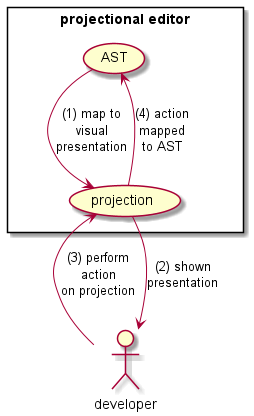
\includegraphics[width=0.35\textwidth]{Sections/images/projections.png}}
    \caption{Projectional editing loop. TODO: comparison with Parsing}
    \label{fig:projectionalEditing_loop}
\end{figure}

To perform the above two things have to be defined by language engineers: The Meta-Model and the editor.

The meta-model, analogous to the abstract syntax, describes the node concepts and connections used to build the hierarchical structure that is the AST.
This hierarchy can have references to nodes in other branches, so it is a graph although named a tree.
The AST is stored independently of the concrete syntax, often using a database, XML or a proprietary file format.
Rules of the meta-model, such as type systems or scoping rules, must also be described.

Projectional editors avoid the grammars and parsers that define the concrete and abstract syntax in a traditional text-based language.
In text-based languages, the concrete is transformed to the abstract with parsing.
In projectional editing, the abstract is transformed to concrete using a projection engine that uses projection rules.

Editors combine the projection rules and the gestures or actions that will create a change request to the AST.
They are analogous to a concrete syntax.

One of the actions can be typing text. 
However, every string is recognized when entered.
Thus, there is no tokenizing.
Text enters into the templates defined by the editor and a newly derived projection displays the adjusted underlying AST to the developer.

The projection uses graphical elements to represent the representation.
Although often appearing textual, each of the text elements are references to nodes in the AST.

Developers can only interact with the editor via the rigidly controlled code completion menus or gestures and actions.
She builds the AST directly from each interaction she has with the editor.

Nodes are instances of the concepts defined in the meta-model.
Each node has a unique id and points to its defining concept.
It is unambiguous.
References are first-class and defined by the id rather than resolved by name, as in parser-based languages.
Disambiguation happens at the time of input, as the developer chooses from limited legal inputs.

The separation of the abstract and concrete allows the language engineer to implement multiple projections of the same model, using different notations, each node of the AST taking having the design she envisions.
The pattern used for projection is similar to MVC, so multiple views of the program can be visible and updateable simultaneously.

Graphical modelling tools, for example for UML modelling, could be seen as specialized implementations of projectional editing.
These modelling tools do not store pictures of the UML diagrams and then parse them to create an AST.
Instead, they store the model, often with extra information about the visual layout, and the image of the UML is projected to the modeller to edit.
Projectional editing generalizes this approach to projecting any notation defined by the language engineer.

\subsection{History of Projectional Editing}

Here follows an incomplete and inconsistent history of projectional languages.

In the '70s and early '80s, researchers created several applications for research into the realm of structured editors.
Some examples were: MENTOR\cite{donzeau1980programming}, Incremental Programming Environment\cite{medina1981incremental}, GANDALF\cite{NotkinDavid1985TGp}, Cornell Program Synthesizer\cite{teitelbaum1981cornell}, and Synthesizer Generator\cite{reps2012synthesizer}.
These language-based program editors could force syntactically correct programs through the knowledge of the language.
These were the precursors to the modern projectional editors. 
They worked by providing templates for each abstract computational unit of the language.
First, one would choose the concept and then fill out the placeholders.

These tools were not good at editing textual notations, which led to a poor user experience.
When they attempted to fix this, for example, in the Synthesizer Generator, they reintroduced parsing to parts, which took away many of the advantages of direct editing of the AST.

In the late '90s and early '00s, the first forays into commercializing a more generalized version of structured editors, the projectional editors, began.
First, Intentional Domain Workbench, inspired by Charles Simonyi's 1995 essay ``The Death of Computer Languages, The Birth of Intentional Programming''\cite{simonyi1995death} the IDW was the product of the company Simonyi founded in 2002, Intentional Software. 
The Intentional Programming paradigm spotlighted the projectional editing domain, taking it out of the universities and into practice.
However, as it was a closed sourced and expensive product, thus not many papers were written about it.
In 2017, as part of an ``acquihire'', Microsoft bought Intentional Software for its employees and let the product die.

Inspired by a call to action for Language orientated programming\cite{dmitriev2004language} JetBrains embarked in 2004 on a mission to build a product to fulfil that ideal.  
Meta Programming System (MPS) was the outcome of that journey.   
Language engineers created the languages mbeddr, PEoPL, and Realaxy using the MPS platform.  
It currently has an active community of developers and projects both in academia and in the commercial world. 
We chose this tool to be the basis of our projectional editing experiments. 
We will talk about it at greater length in section \ref{section:MPS}.

The last decade has produced a few smaller projectional workbenches.
There are a few open-source, small team projectional projects.
In 2013 several projectional language workbenches joined MPS in the Language Workbench challenge\cite{erdweg2015evaluating}.
These included M\'as, a web-based projectional editor, which is no longer with us\cite{MasPostMortem}.
Whole Platform\cite{WholePlatformProductPage} is a projectional language workbench plugin for Eclipse.
Cedalion\cite{lorenz2011cedalion} provides another projectional IDE, specializing in internal DSLs.

More recently there have been some interesting products that intersect the projectional domain.
Deuce\cite{hempel2018deuce} and Gentleman\cite{lafontant2020gentleman_SLR} are two recent projection editors that have recently emerged from academia.
The final two mentions in our incomplete history are a little out of left-field. 
Google's Blockly\cite{Blockly_ProductPage} is a tool for making structural editor languages, but only in a block format.
This can create languages similar in style to the scratch language. 
Blueprint visual scripting, a part of the Unreal Engine, is a visual programming languages for building concepts such as levels or game assets.
Examples of Blockly and Blueprint can be seen in figures \ref{fig:blockly} and \ref{fig:Blueprint} respectively.

\begin{figure}[H]
    \begin{subfigure}{.50\textwidth}
      \centering
      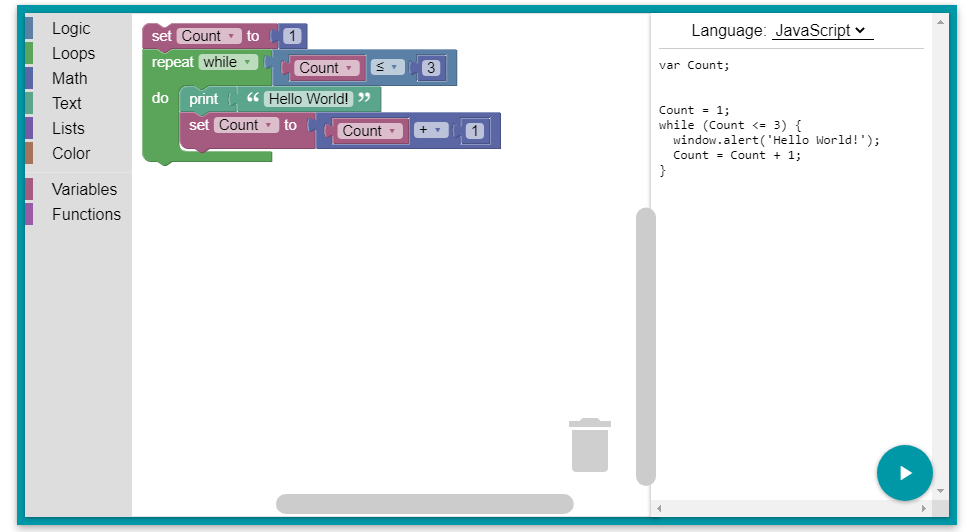
\includegraphics[width=.95\linewidth]{Sections/images/blockly.png}
      \caption{Blockly}
      \label{fig:blockly}
    \end{subfigure}%
    \begin{subfigure}{.50\textwidth}
      \centering
      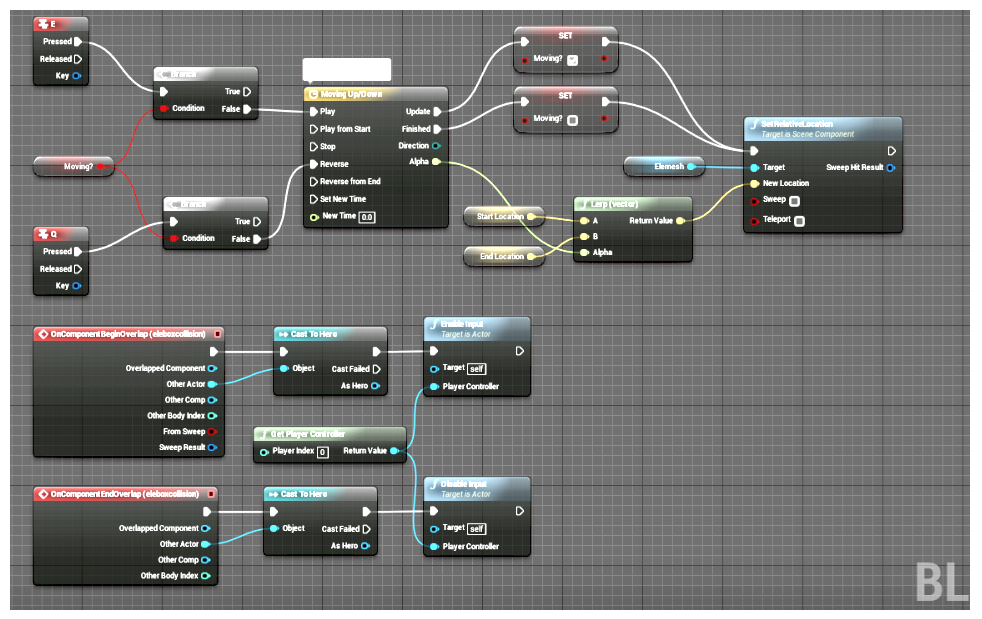
\includegraphics[width=.95\linewidth]{Sections/images/blueprint.png}
      \caption{Blueprint}
      \label{fig:Blueprint}
    \end{subfigure}
    \caption{Leftfield projectional editors}
    \label{fig:leftfield}
\end{figure}

\subsubsection{What Advantages Does Projectional Editing Bring?}

Projectional editing gives advantages both to the language engineer and the program developers.
There is a lot of crossover and repetition between papers written on projectional editing as to the advantages it brings.
To that end, what follows is a synthesis of several papers as to the advantages that projectional editing claims.
Rather than attributing each advantage to each paper, we have made a reference table of papers proclaiming said advantage.
This is table \ref{table:Projectional_Advantages}.

\begin{table}[h]
    \begin{center}
        \begin{tabular}{ |l | c | l | } 
            \hline
            Advantage                   & \#& Paper(s)   \\
            \hline
            Exploratory programming     & 5 &\cite{klimevs2016domain,ratiu2017experiences,volter2010language,voelter2014towards,hosseinkord2021code}                                                                        \\
            Correctness-by-construction & 7 &\cite{voelter2013dsl,ratiu2019fasten,ratiu2012language,klimevs2016domain,berger2016efficiency,klimevs2016domain,vysoky2018ingrid}                                          \\
            Rich notation               & 22&\cite{pech2021jetbrains,voelter2014supporting,voelter2010language2,voelter2015using,voelter2010embedded,guttormsen2017consistent,voelter2010domain,wortmann2016domain,klimevs2016domain,voelter2013mbeddr,berger2016efficiency,simonyi2006intentional,voelter2016efficient,vysoky2018ingrid,pech2013jetbrains,volter2010language,voelter2014projecting,ratiu2018taming,voelter2015towards,voelter2014towards,simonyi1995death,voelter2019using} \\
            Mixed notation              & 8 &\cite{ratiu2017experiences,voelter2010language2,voelter2015using,voelter2010embedded,guttormsen2017consistent,volter2010language,voelter2014supporting,voelter2014towards}              \\
            Multiple views              & 9 &\cite{klimevs2016domain,voelter2016efficient,voelter2010language2,volter2010language,voelter2010embedded,voelter2010domain,vysoky2018ingrid,volter2010language,voelter2014supporting}   \\
            Language composition        & 23&\cite{voelter2013dsl, meacham2020adaptivevle, ratiu2019fasten, pavletic2013extensible,voelter2011language,guttormsen2017consistent,berger2016efficiency,voelter2016efficient,voelter2010embedded,ratiu2012implementing,volter2010language,voelter2010language2,voelter2012mbeddr,voelter2011product,voelter2013requirements,voelter2014supporting,voelter2014towards,voelter2015using,voelter2019using,simonyi1995death,vysoky2018ingrid,pech2013jetbrains,voelter2015towards} \\
            IDE functionality           & 4 &\cite{klimevs2016domain,voelter2010embedded,voelter2010language2,voelter2010embedded}                                                                                                \\
            Language evolution          & 1 &\cite{schindler2016language} \\
            Ancillary data              & 5 &\cite{voelter2011product,voelter2013requirements,voelter2019using,volter2010language,voelter2010language2} \\
            \hline
        \end{tabular}
    \end{center}
    \caption{Papers describing advantages}
    \label{table:Projectional_Advantages}
\end{table}

 
\paragraph{Exploratory programming}
As with their progenitors, syntax-directed editors, modern projectional editors help guide a developer unfamiliar with a language.
With their rigid syntax and predefined layout, the editors only allow editing within specific cells of the editor.
This template style means that the developer does not have to worry about the significance of spacing or indentation.
Minutiae of syntactic adornments, such as statement ending semi-colons or enclosing matched brackets, are also not interfering with her exploration of the language space.

When creating code, the editor only presents the developer with legal options within the current context.
As the projection is context-aware, with relevant actions and options suggested and irrelevant ones removed.
Thus, it is easier for the developer to explore what the language allows her to choose.
Intelligent code completion does not have to be limited to single nodes.
Inserting whole subtrees allows the developer to explore the larger structures of the language.

\paragraph{Correctness-by-construction}
A projectional editor prevents her from writing syntactically incorrect code by controlling the interaction between the developer and the AST.
The whole class of syntactical errors is made impossible, with the developer relieved to think about special characters and layout.
Typing and scoping errors are removed by only allowing validly typed and scoped options for the developer.

The developer can only select statements that are legal in the context of the location within the AST.
Code does not have to be disambiguated, as this happens at the time of entry by the developer.
If multiple items share the same notation in the editor, the developer chooses the relevant item, thus resolving the ambiguity to what she means rather than what the parser thinks she means.

\paragraph{Rich notation}
Constraints associated with textual parsing do not affect the choice of created projections. 
This freedom opens up diverse otherwise tricky or impossible to parse notations.
Examples include tabular, mathematical expressions and symbols, diagrams, trees, images, forms, prose, sub- and superscript.
Any visual form or shape that can map onto the AST can represent the program in an editor.

With these notations, one can better reflect the semantics of the program domain, which should aid comprehension.
Mathematics has a rich history of use of notation.
When writing a DSL for the Mathematics domain, the domain experts can interact with it in the centuries-old language of their domain.

Of course, the projections can also be projections of text.
Textual projections are often the appropriate projection type if the developer interacting with the language's domain expertise is parser-based languages.

\paragraph{Mixed notation}
As no parsing is required and ambiguity is not an issue for the underlying AST, it is straightforward to combine different forms of rich notation.
With all notations working on the same editor infrastructure, embedding mathematic symbols within textual projections, within tables within graphical representations is a simple coding pattern.

\paragraph{Multiple views}
With the AST being the stored artefact rather than the notation, projectional editing allows the language engineer to define multiple views on the same model optimised for different tasks.
In Software architecture, one presents different views to different stakeholders based on their interests.
Similarly, projectional editing can present experts with various domain expertise views on the model that reflect their needs.
A developer can switch between different node projections within a larger projection to find the one that best suits their current task.

Because the architecture of a projectional editor follows the principles of model-view-controller, it is possible to have multiple simultaneous views of the model.
These multiple views allow the developer to update a projection optimised for writing and immediately see its effect in a projection optimised for understanding.

\paragraph{Language composition}
Parser-based languages can support some modularization and composition, but a projectional editor allows easy and extensive modular language extension and composition.
This ability results from the disambiguation of the nodes of an AST at the time of entry.
If two items with the same syntax are available at the same place, then the user will choose the one they require, and therefore the node has an explicitly chosen meaning.

The composition of independently developed languages does not suffer from the syntactic or keyword clashes they would in two grammar defined languages.
Because of the lack of ambiguity, every node referencing the concept that defines it, these languages, when put together, will not have structural or syntactic issues.

Language composition can involve extending an existing language or embedding other languages in a host language without modifying its definition.
The ease of composition and extensions allows building more significant languages out of smaller modules.

\paragraph{IDE functionality}
Developers in mature languages are used to the functionality of mature IDEs.
These functionalities include syntax highlighting, intelligent code completion or suggestion, and static analysis for errors and validation.
As projectional languages store the AST rather than the concrete syntax, they require an IDE to edit.
Because of this, when a language engineer designs the language, she also has to design the IDE.

A projection always knows its context because it comes from the AST.
When the editor already knows the meaning of the node it represents, syntax highlighting is simple.
Knowing its context makes it much simpler to suggest intelligent code completions.

Always having a complete AST makes it much easier to validate scope, typing and other hard to implement code validators.

\paragraph{Language evolution}
Parsing complicates the evolution of languages. 
For example, adding a new reserved word is difficult without breaking existing code.
Extending a language with new capabilities and syntax in projectional editing is simple.
If the change is syntactic, then the language engineer has to update an editor.
If there is a semantic change, then the language engineer can write a migration in the language to transform a node of one concept to a different type, and the developer would have to run that migration on their code.

\paragraph{Ancillary data}
Data added to nodes can augment the AST.
This data is useful for tasks such as documentation, requirements traceability and product line feature dependencies.

\subsubsection{What are the Disadvantages of Projectional Editing?}
Whilst fewer papers proclaim the disadvantages of projectional editing, we repeated the approach of the previous section.
Thus, we have synthesised the disadvantages from papers in the following sections and listed citations for these ideas in table \ref{table:Projectional_Disadvantages}.

We do not consider that the dearth of disadvantages discussed as evidence of projectional editing's superiority.
Our best guess is that those who do not find projectional editing useful do not write papers about it.

\begin{table}[h]
    \begin{center}
        \begin{tabular}{ |l | c | l | } 
            \hline
            Disadvantage               & \#& Paper(s)   \\
            \hline
            Low adoption               & 4 &\cite{vysoky2018ingrid,voelter2015using,voelter2015towards,voelter2014projecting} \\
            Unnatural user experience  & 11 &\cite{vysoky2018ingrid,voelter2015towards,voelter2014towards,voelter2012mbeddr,voelter2014projecting,berger2016efficiency,voelter2016efficient,voelter2010embedded,voelter2010language2,schindler2016language,voelter2014supporting} \\
            Ambiguous syntax           & 1 &\cite{guttormsen2017consistent} \\
            Inflexibility              & 2 &\cite{voelter2014towards,voelter2014supporting} \\
            lack of integration with text ecosystem & 5 &\cite{voelter2012mbeddr,voelter2014towards,voelter2012mbeddr,voelter2014projecting,voelter2014supporting} \\
            Learning curve             & 5 &\cite{voelter2010language2,pech2013jetbrains,voelter2012mbeddr,voelter2014towards,voelter2015using,prinz2021teaching} \\
            Vendor lock\-in            & 2 &\cite{voelter2010embedded,voelter2010language2,tomassetti2020reflections} \\
            \hline
        \end{tabular}
    \end{center}
    \caption{Papers describing projectional editing disadvantages}
    \label{table:Projectional_Disadvantages}
\end{table}

\paragraph{Lack of adoption}
The ideas that proceeded projectional editing - the structured or syntax-directed editor - have been around since the early 1970s yet have failed to be adopted widely.
This argument is a bit of a tautological one, as the low adoption is perhaps an outcome of the other disadvantages of projectional editing.
However, low adoption can lead to a self-reinforcing process, where lack of adoption prevents further adoption.

\paragraph{Inconvenient or unnatural editing}
Early attempts at projectional editing presented an inconvenient and unnatural user experience when coding.
These usability challenges, exemplified by the tedious manner of entering code as per the tree's order, compare poorly to parser-based languages.

This lousy reputation continues, despite massive improvements in projectional editors.
Whilst there is no debate that projectional editing feels different, some question whether this inconvenience is an intrinsic property or a result of developers, through years of experience, being used to text-based programming.

Modern projectional editors, when using a textual projection, face an ``uncanny valley'' issue.
Whilst trying to simulate a text editor, the developers start to expect all of the functionality of the text-based IDEs.
This expectation is a particularly weak spot, especially regarding granularity and restrictions of cursor movement, insertion, deletion, selection, copy and paste, and other interactions with the text.

\paragraph{Ambiguous syntax}
One of the selling points of projectional editing, especially concerning language composition, is that there can be no ambiguous syntax.
While this may be true for the AST, it is not so for the developer who reads this code on the screen.
If one combined Drools and Basic rather than Java, the developer might become confused about which language the ``Then'' keyword refers to when she read it.
Thus writing ambiguity is replaced by reading ambiguity.

\paragraph{Inflexibility}
A developer using a projectional editor has no flexibility in code layout. They may feel they require this for enhanced readability.
The flexibility of the layout is entirely in the hands of the language engineer when she determines the projection rules.

\paragraph{Integration with the text based world}
Projectional editors do not store the definition of the program in the form of a plain-text implementation in the concrete syntax.
Instead, the AST is stored and serialized in a format that is not human readable, such as XML.

This different format of program storage leads to an issue with integration with the text-based ecosystem.
This ecosystem is extensive, as text-based coding has been popular since the 60s.
Two notable examples are text diffing, especially where branch merging is concerned and code sharing.
The diffing issue within projectional editing tools is solved.
However, as code-bases often span multiple programming languages and tools, the difficulty of integrating projectional diffing into the software development workflows is still a real problem.

Textual source code can be shared simply by email or on websites. 
This sharing, however, is not easy with projectional code.

\paragraph{Learning curve}
For the language engineer, the necessity to develop an editor with a good user experience is much harder work than defining a grammar for a parsed language.
The learning curve for the language engineer is significant, as, by default, she has to think also of the IDE development.

For the developer, especially one with an extensive text-based experience, the different editing style takes some getting used to.

\paragraph{Vendor lock-in}
The nature of projectional editing is that what one edits is a projection of the AST, and therefore an IDE is needed to do the projecting and language definition.
Organisations thinking of going the projectional route for their DSLs may fear being locked into a specific concept implementation.
To be able to use previously developed languages would require using the same toolset.
Changing to a different toolset for language design would require a significant re-skilling effort.

\section{What is MPS?}
\label{section:MPS}

Language workbenches (LWB) are tools to help language engineers create languages, particularly domain-specific languages (DSL).
Fowler\cite{Fowler_lwb} popularised the term LWB in a 2005 article.

Meta Programming System (MPS) is an open-source LWB that assists in the creation of projectional languages.
It started in 2003 by JetBrains and was introduced to the world in Dmitriev's 2004 Paper ``Language Orientated Programming: The Next Programming Paradigm''\cite{dmitriev2004language}.

As discussed in Section \ref{section:WhatIsPE}, when creating a projectional language, one must define the language and how one interacts with it.
In MPS, the language engineer defines languages, including their interactions.
Developers create programs using these languages.
The language engineer can extend languages.
The developer can mix the languages she uses.

The following is an overview of how MPS implements the ideal of a projectional language.
It is also the structure of this section: 

\begin{itemize}
    \setlength\itemsep{0em}
    \item Abstract syntax
    \begin{itemize}
        \setlength\itemsep{0em}
        \item Structure
        \item Behaviors\footnote{When referring to its use in the MPS workbench, consistent with their use, we use the American spelling - Behavior.}
        \item Constraints
        \item Type system
    \end{itemize}
    \item Concrete syntax
    \begin{itemize}
        \setlength\itemsep{0em}
        \item Editors
        \item Intentions
    \end{itemize}
    \item Generators
    \begin{itemize}
        \setlength\itemsep{0em}
        \item Model-to-Model
        \item Model-to-Text
    \end{itemize}
\end{itemize}

MPS defines the different aspects of the language definitions with small, declarative DSLs.
These are bundled together into what they term Aspects.

\subsection{Abstract Syntax: Structure}
Structure is what determines the abstract syntax of a language.
The most important item available in a Structure Aspect is the Concept.
Instances of concepts are called nodes.
With these nodes, the developers construct their programs.
When referring to a program in MPS, we are talking about its stored abstract syntax tree (AST).

In principle, a concept contains three types of things:
\begin{enumerate}
    \setlength\itemsep{0em}
    \item Properties: these primitives are integer, boolean, string, or enum items and are similar to leaf values.
    \item Children: these are other concepts, or collections of them, similar to subtrees.
    \item References: these are relationships with other nodes in the AST. These turn the tree into a graph.
\end{enumerate}

Concepts follow some object orientated (OO) traits, such as subtype, being abstract, and implementing interfaces.

One of these Concepts must be a root node. 
Otherwise, there is nowhere for a program to start.

Other items available in the Structure Aspect are the Interface Concept, the Enumeration, the Constrained Data Type, and the Primitive Datatype.
\footnote{At the time of writing, we are unaware whether Data Type and Datatype are semantically different or that the different naming is just a style choice.}

Thus, the Structure aspect defines how the AST can be structured.

Figure \ref{fig:concept_example} shows a concept with three children that implements two interfaces.
The first line names the concept and which concept it extends.
By default, all concepts extend \texttt{BaseConcept}.
The next two lines shows the interfaces it implements.
This concept is not rootable, and therefore cannot be instantiated as a file in a solution.
the alias and short description override what will be shown in menus instead of \texttt{RuleStatement} and its fully qualified name.
This concept has no custom properties or references.
It has three children.
The attributes child contains one and only one \texttt{RuleAttribute} node.
Outcomes also contains only one child node, this one of type \texttt{StatementList}.
The conditions child has a collection of \texttt{AbstractCondition} nodes.

\begin{figure}[h]
    \centering
    \fbox{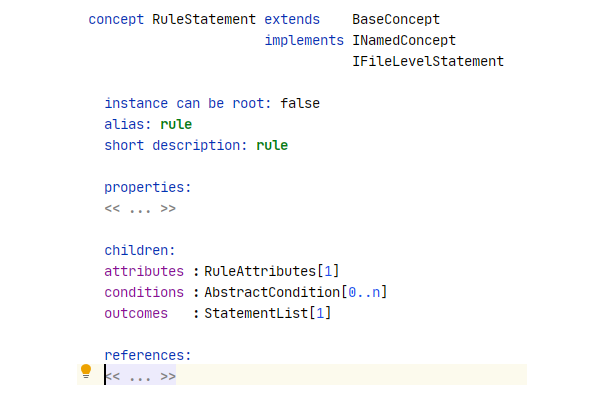
\includegraphics[width=0.66\textwidth]{Sections/images/concept_example_P.png}}
    \caption{Concept example}
    \label{fig:concept_example}
\end{figure}
 
\subsection{Abstract Syntax: Behaviors}
OO design usually bundles together data and methods that can act on that data.
Concepts are analogous to the data part of this equation.
Behavior fills the role of the methods in the OO analogy, defining the functionality called from instantiated nodes and static methods called from the Concept.
The Constructor is a specialised method in a Behavior, filling the same role as a constructor in OO.

The methods have public, private, or protected visibility.
If the Concept to which the Behavior refers is abstract, the Behavior itself can contain abstract methods.
Abstraction, variable visibility, and inheritance allow a sort of polymorphism.
If a virtual method is declared, then it can be called polymorphically.

Figure \ref{fig:behavior_example} shows a constructor added to a Concept to initialise its children.
It has a method to allow other nodes to interrogate the condition of it having attributes.

\begin{figure}[h]
    \centering
    \fbox{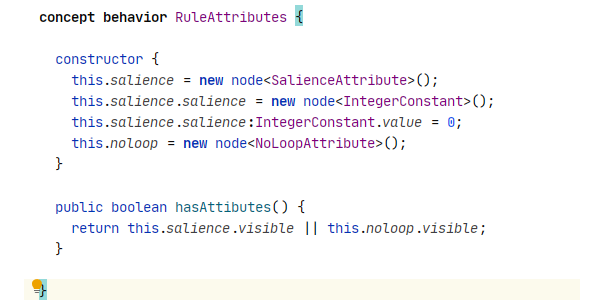
\includegraphics[width=0.66\textwidth]{Sections/images/behavior_example_P.png}}
    \caption{Behavior example}
    \label{fig:behavior_example}
\end{figure}

\newpage
\subsection{Abstract Syntax: Constraints}
A Constraints aspect adds further structural restrictions to a Concept.
Constraints primarily define scope by controlling if another node can be a child, a parent, or an ancestor of this node.
A Constraint can also prevent badly formed properties, children, or references.

Figure \ref{fig:constraint_example} shows an example of a scope restraint that only allows local variables declared within the same rule or global variables declared in the same file.
 
\begin{figure}[h]
    \centering
    \fbox{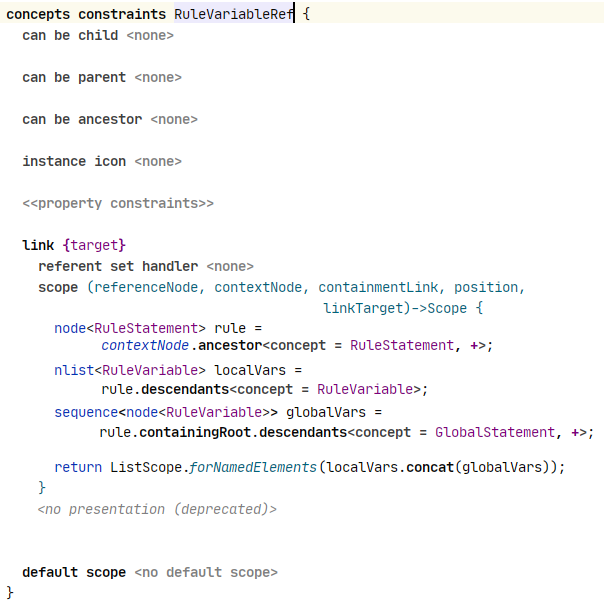
\includegraphics[width=0.66\textwidth]{Sections/images/constraint_example_P.png}}
    \caption{Constraint example}
    \label{fig:constraint_example}
\end{figure}

\subsection{Abstract Syntax: Type System}
The Type system aspect and the constraints aspect together represent the static semantics of the language.
This aspect is for the computation and evaluation of types of variables, expressions, and statements.

Rules that are available to calculate and enforce the type system include inference, subtyping, comparison and substitute type rules.

Figure \ref{fig:typesystem_example} shows an inference rule that ensures that the calculated type of the import statement matched that of its child ``type''.

\begin{figure}[h]
    \centering
    \fbox{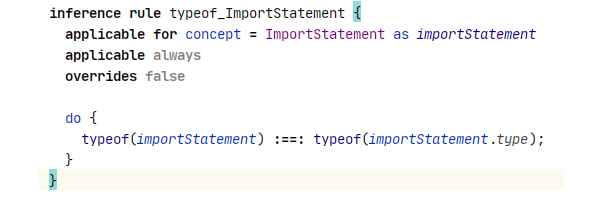
\includegraphics[width=0.66\textwidth]{Sections/images/typesystem_example_P.png}}
    \caption{Type system example}
    \label{fig:typesystem_example}
\end{figure}

\subsection{Concrete Syntax: Editors}
Editor aspects define the notation of the nodes.
In effect, it is the user interface of the language, projecting the AST to the developer.
An editor is a swing panel that renders a tree of editor cells.
A Concept can have multiple editors, thus offering multiple views on it.

The definition of the options available to the developers through menus also happens within the Editor Aspect. 
The choice the developer makes transforms the existing AST.

Additionally, the behaviour of interactions can be defined, such as what will happen to the AST when a particular keypress or editor action occurs at a particular location.

Figure \ref{fig:editor_example} shows a component with a projection for the Concept shown in Figure \ref{fig:concept_example}.

\begin{figure}[h]
    \centering
    \fbox{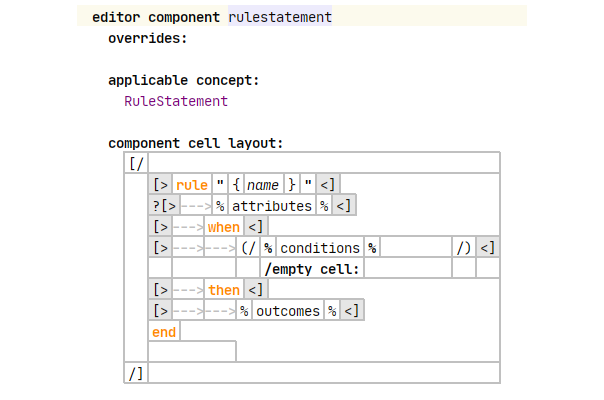
\includegraphics[width=0.66\textwidth]{Sections/images/editor_example_P.png}}
    \caption{Editor example}
    \label{fig:editor_example}
\end{figure}

\subsection{Concrete Syntax: Intentions}

In projectional editing, the IDE is a part of the concrete syntax.
Intentions make context-aware suggestions for automatic changes to the program to the developer.
Figure \ref{fig:intention_example} shows an intention that allows the developer to add, remove or edit a property based on its current value.

\begin{figure}[h]
    \centering
    \fbox{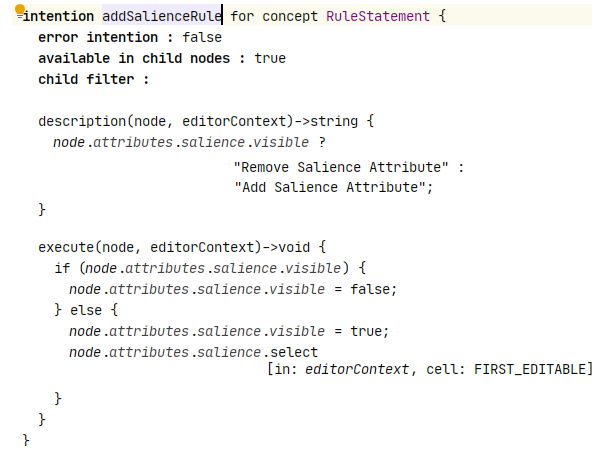
\includegraphics[width=0.66\textwidth]{Sections/images/intention_example_P.png}}
    \caption{Intention example}
    \label{fig:intention_example}
\end{figure}

\subsection{Generators}
In our implementation we will not be using generators.
However, as they are an important part of a typical language implementation, we will discuss them briefly here.

There are two types of generators, the Model-to-Text generator and the Model-to-Model generator.

Whilst designing a language is nice, it should be able to do something. 
Without doing so, it has no semantic meaning.
It is possible to create interpreters that can use the AST generated by MPS.

However, the most common modality for MPS is to generate, via a model-to-text generator, an output that gets compiled and run by commonly known environments.
The output stage of generation is called TextGen.
It defines how a node becomes runnable code in plain text.

Base level languages will have text generation.
Most DSLs will perform model-to-model conversions, eventually converting to a base language.
These intermediate stages are known as Generator Aspects.
They transform code written in one language to another.

In MPS, a Concept can have multiple generators aimed at different base level languages, such as Java (using MPS BaseLanguage), C (using mbeddr) or XML.



    \chapter{Methods}
\label{chapter:Methods}

To answer the research questions from section \ref{section:Research_Questions}, we persued three approaches.
We answered the question ``What is the current state of language workbenches supporting projectional editing?'' by conducting a systematic literature review (SLR), which we describe in section \ref{section:Method_systematic_review}.
We followed two linked approaches for the question ``Which projections can help developers get appropriate feedback about rules?''.
Firstly, using Action Design Research (ADR), we implemented Drools as a projectional editor, and then some projections that users can edit.
We describe this approach in section \ref{section:Method_action_research}.
Then, as we detail in section \ref{section:Method_survey}, we presented our findings to experienced Drools users through a questionnaire survey to validate this approach.

\section{Method: Systematic Review}\label{section:Method_systematic_review}

To answer the first Research Question, ``what is the current state of Projectional Editing?'', we conducted a systematic literature review.
Hereafter, we describe the method we undertook.

To carry out this review we followed Kitchenham's\cite{Kitchenham_2015} advice on systematic review protocol validation, (see appendix \ref{appendix:protocolValidation} for the exact checklist we used).

\subsection{Motivation}
The motivation that preceded this research was a requirement to understand if projectional editing was an idea that was worth investigating.
Through our background research we saw an interest in the precursors to projectional editing in the late 70's through to the mid 80's.
This seemed to be abandoned until the mid 90's following Charles Simonyi's treaties on Intentional programming.
This did not lead to a swell in academic research as his companies product, Intentional Domain Workbench was a closed commercial product.
There seemed to be a burst of academic interest after the release of JetBrain's OpenSource Meta Programming System (MPS) in the late 2000's.

Is there a need for a study of this topic? 
We believe, at least in the microcosm of this master's project it is helpful to know whether we are researching in an area that is dying of vibrant.

For the wider community, there does not seem to be any systematic reviews specifically about projectional editing, let alone recently.
This study is not extending any previous Systematic Review as, although there were literature surveys and mapping studies covering some adjacent fields, no SLRs were found.
Thus we believe it may be useful for those in the language engineering research community to bring together all current research in the area of projectional editing in one place.

\subsection{Research Question}
This paper we only have one research question to synthesize the findings of scientific papers towards.
This is ``What is the current state of Projectional Editing?''

This question for us can be broke down into:
\begin{itemize}
    \item \textbf{Sub Question 1} ``Is there current research in the area of projectional editing?''
    \item \textbf{Sub Question 2} ``What tools are currently being used for research?''
    \item \textbf{Sub Question 3} ``What is the sentiment in papers currently discussing projectional editing?''
\end{itemize}


\subsection{Search Strategy}

The search process is automated as SLRs require a high level of completeness, which cannot be effectively achieved manually.
Our first major decision was whether to engage in creating a quasi-gold standard as advised by Zhang\cite{Zhang_2011}.
Zhang noted that the ad-hoc nature of search strategies in SLRs has limitations.
We executed a preliminary ad-hoc search to try and ascertain the extent of the research space.
Upon satisfying ourselves that it was small enough, we rejected the Quasi-Gold standard as overkill for our requirements.

The search terms we landed on were as follows:
{\obeylines\obeyspaces
\texttt{
    ``PROJECTIONAL EDITING'' 
       OR 
    ``PROJECTIONAL EDITOR'' 
}}

This is to be adjusted to fit the query syntax of the various search engines.

As most Research Search engines offer the option of date ranges, and to save the effort of excluding later we also used the date range to eliminate unnecessary paper at the automated search stage.
Our research question we are specifically looking at the current state of projectional editing.
A design decision of many research search engines is that date ranges can often only be defined in whole years.
When designing our search strategy, it was near the beginning of 2021, and thus we feared that this would be too small a search space, thus we set our date range to be from the beginning of 2020 to present.
For the sake of reproducibility, it is advised to remove any papers after 31st July 2021.

The Search Engines used are shown in table \ref{table:searchEngines}.

\begin{table}[H]
    \begin{center}         
        \begin{tabular}{|l||l|}
            \hline
            ACM digital library       & Google Scholar       \\
            \hline
            BASE                      & CORE                 \\
            \hline  
            IEEE Xplore               & ISI Web of Science   \\
            \hline  
            Microsoft Academic        & Science.gov          \\
            \hline  
            Wiley InterScience        & SCOPUS               \\
            \hline  
            Semantic Scholar          & SpringerLink         \\
            \hline  
        \end{tabular}
    \end{center}
    \caption{Search Engines Used}
    \label{table:searchEngines}
\end{table}

Once we have filtered the automated search through the criteria of the selection stage, we will use that as our starting set for snowballing.
Our filtering will be done before the quality of the papers has been assessed, as we feel that excluding papers on quality of primary study issues may artificially limit the network of potential papers.
Our snowballing procedure shall follow the advice of Wohin\cite{Wohlin_2014}.
This is the idea of using the reference lists from our start set and applying the same selection criteria to these.

Where possible we will get the forward snowballing papers from the ``cited by'' functionality of Google Scholar.
Because of the range of the search being to present, all papers that cite the target paper will fall within our criteria.
For backward snowballing we will manually filter the bibliography section of the selected papers, selecting any paper published in 2020 or 2021

After gathering all the papers from the forward and backward snowballing we will again apply the selection criteria.
This process will iterate recursively until no new papers are found.
All of the papers not excluded in each iteration will be the basis for the quality of primary studies filtering stage.

After the final iteration, as a final step the selected papers will have a deeper scan.
This is to verify our initial scan that the papers met our inclusion criteria, before moving on to the quality assessment.

\subsection{Study Selection}

The inclusion criteria are:
\begin{itemize}
       \item Studies are about or mention projectional editing or one of it's synonyms
       \item It is published in during the period 2020\-2021
\end{itemize}

The exclusion criteria are:
\begin{itemize}
       \item Books and grey literature
       \item not English
       \item no full text available
       \item papers with serious issues with grammar or vocabulary
       \item not a previously selected paper
       \item not a paper about a previously reported on study
\end{itemize}

If multiple papers look at the same study with different approaches, then the data will be aggregated in the synthesis stage.

As a lone researcher, we must be aware of bias in positively including relevant papers and excluding irrelevant papers.
We will follow Kitchenham's suggestions to overcome such bias:
\begin{itemize}
       \item Test-retest 
       \begin{itemize}
              \item We will assess the papers once (on title abstract and keywords) against the inclusion and exclusion criteria.
              \item Save all the suggested results
              \item Assess the papers again three days later in a different order to the first  
       \end{itemize}
       \item If there are disagreements, we will use Cohen's Kappa agreement statistic\cite{Cohen_1960} to see if the process needs to be refined.
\end{itemize} 

If our searches appear to be too large for a lone researcher, we will turn to text mining.
We will be cautious to use this.
O'Mara-Eves et al.'s systematic review of text mining in systematic reviews\cite{OMara-Eves_2015}, recommends that this can be used for prioritization, but finds that for exclusion screening, although promising, it is not yet proven.

An SLR is interested in studies rather than papers.
There is a many-to-many relation between papers and studies.
We will review the selected papers to note when this has happened in our results to make sure studies do not get over or undercounted.

\subsection{Quality of Primary Studies}
To discover explanatory reasons for why there may be differences in study results, and to weigh how valuable specific studies are, we will assess the quality of the selected studies.

To try and avoid a Results Section bias we will be operating a results-blind quality assessment.
Study quality will be based on the methods section of the papers only.
This bias is threatened because results are summarized in the abstract.
The study quality will not be measured until after the selection process is complete, though it will, in part be carried out before the selection re-test.
list of papers will be randomly sorted before assessing for quality.

For EBM studies there are some well-known hierarchies of evidence for study quality thresholds such as the CRD Hierarchy of Evidence\cite{Cochrane_2019}.
Kitchenham in, Procedures for Performing Systematic Reviews\cite{Kitchenham_2004_2}, suggests the hierarchy shown in table \ref{table:hierarchy}

\begin{table}[H]
    \begin{center}   
    \resizebox{\textwidth}{!}{%
      
        \begin{tabular}{|l||l|}
            \hline
            Rank     & Description                                                                                         \\
            \hline
            \hline
            1        & Evidence obtained from at least one properly designed randomized controlled trial                   \\ 
            \hline  
            2        & Evidence obtained from well-designed pseudo-randomized controlled trials                            \\
                     & (i.e. non-random allocation to treatment)                                                           \\
            \hline  
            3-1      & Evidence obtained from comparative studies with concurrent controls and allocation not randomized,  \\
                     & cohort studies, case-control studies or interrupted time series with a control group                \\
            \hline  
            3-2      & Evidence obtained from comparative studies with historical control, two or more single-arm studies, \\
                     & or interrupted time series without a parallel control group                                         \\
            \hline  
            4-1      & Evidence obtained from a randomized experiment performed in an artificial setting                   \\
            \hline  
            4-2      & Evidence obtained from case series, either post-test or pre-test/post-test                          \\
            \hline  
            4-3      & Evidence obtained from a quasi-random experiment performed in an artificial setting                 \\
            \hline  
            5        & Evidence obtained from expert opinion based on theory or consensus                                  \\
            \hline  
        \end{tabular}}
    \end{center}
    \caption{Study design hierarchy for Software Engineering}
    \label{table:hierarchy}
\end{table}

These different types of study have different quality assessment criteria.
As the nature of our research questions is not likely to attract randomized or pseudo-randomized controlled trials or experiments, our quality assessment checklists are created with comparative studies and case series in mind.
To assess the strength of each primary study we used the checklists shown in appendix \ref{appendix:QualityAssesmentChecklist}.
The checklists were based on a subset of the questions suggested in Keele's guidelines on SLRs\cite{keele2007guidelines}, which in turn extracted questions from previous mostly medical systematic reviews.
Where necessary the selected questions were modified for software engineering.

These checklists are addressed toward general research.
In Software Engineering many studies that fall under what Gregor\cite{gregor2006nature}, in ``A Taxonomy of Theory Types in Information Systems Research'' calls ``Type V: Theory for Design and Action''.
The checklists do not address this type of research well.
On investigation into how others SLRs conduct quality assessment we did not find a solution to this issue.
Therefore we will continue with the checklists as in the appendix, using the checklists for Case Study for Type V research papers.
We will take this into account before dismissing results of this type on basis of their quality score.

As this study will be carried out by a lone researcher, there is no need to have a process for disagreements.
To check on the bias, several papers will be randomly selected and assessed using the checklist by the academic and the daily supervisors.
Should there be a high disagreement the design of the checklist will be revisited.

The quality checklist is trying to weed out the biases of selection, performance, detection, and exclusion, as well as other threats to the validity of the studies under test.
Validity issues can occur during the design, operation, analysis, or conclusion of an empirical study.

\subsection{Data Extraction}
No data extraction will be necessary for the first sub-question,  ``Is there current research in the area of projectional editing?''.
The fact of the existence of papers that have been verified to be primary studies either into projectional editing theory or practical use of it will be enough to answer the question.

For the question of ``What tools are currently being used for research?'', we shall note each tool discussed specifically with regards to the study being carried out.

Finally, for the sentiment we shall pass each paragraph of the introduction, the discussion and the conclusion through a sentiment analyser and, if the paragraph is pertinent to projectional editing, we will not it's sentiment score.
The sentiment analysis tool we shall use is Microsoft Azure Cognitive Services Text Analytics.
The code to carry out this task is shown in listing \ref{listing:text_analytics}

\begin{lstlisting}[language=Python, caption=Text Analytics code., captionpos=b, label=listing:text_analytics, breaklines=true]

    from azure.core.credentials import AzureKeyCredential
    from azure.ai.textanalytics import TextAnalyticsClient
    
    endpoint = "REPLACE_WITH_CORRECT_ENDPOINT"
    key = "REPLACE_WITH_CORRECT_KEY"
    
    text_analytics_client = TextAnalyticsClient(endpoint=endpoint, credential=AzureKeyCredential(key))
    
    inputfiles = [[ARRAY_OF_FILES_TO_BE_ANALYSED]]
    
    with open('/content/sample_data/sentiment/output_all.txt','a') as outf:
      for sections in inputfiles:
        for section in sections:
          print("Section: {}".format(section),file=outf)
          f = open('/content/sample_data/sentiment/'+section)
          content = f.readlines()
          # for brevity an optimization to deal with 10 document limit is removed
          if len(content) != 0:
            result = text_analytics_client.analyze_sentiment(content, show_opinion_mining=True)
            docs = [doc for doc in result if not doc.is_error]
            for idx, doc in enumerate(docs):
              print("sentiment: {}".format(doc.sentiment),file=outf)
              print("Document text: {}".format(content[idx]),file=outf)
\end{lstlisting}


\begin{table}[H]
	\centering
	\begin{tabular}{|c | l | l | c |} 
		\hline
		\#& Data Type           & Description                                          & RQ     \\ \hline
		\hline
        1 & Study ID            & Unique identifier for the study                      &        \\ \hline
        2 & Title of Study      & The paper name                                       &        \\ \hline
        3 & Year of Publication & Will be either 2020 or 2021                          &        \\ \hline
        4 & Author(s) Names     & Including affiliation                                &        \\ \hline
        5 & Source of Study     & Name Of Online Database/ Digital Library             &        \\ \hline
        6 & Type of Study       & Publication/Conference/Workshop/Symposium            &        \\ \hline
        7 & Name of Venue       & Journal/Conference in which study has been published &        \\ \hline
        8 & Tools in Study      & A list of the tools used                             & RQ 1.2 \\ \hline
        9 & Sentiment           & The sentiment scores from appropriate paragraphs     & RQ 1.3 \\ \hline		
	\end{tabular}	
	\caption{Data extraction form.}
    \label{table:Data_Extraction_Form}
\end{table}

\subsection{Data aggregation and synthesis}
As explained by Kitchenham\cite{kitchenham2015evidence}, in software engineering, primary studies will tend to be too heterogeneous for any statistical analysis.
Synthesizing outcomes from multiple methods will be difficult.
Thus our synthesis will take a narrative approach.

Narrative synthesis is telling a story of the who, how, and why of the success or otherwise of the research.
For ADR research, focus will be on what will help or hinder the adoption of the implementations.
It will also examine how reliable the results are and relationships between the studies.


\newpage
\section{Method: Action Research - Drools in MPS}\label{section:Method_action_research}

Even though Drools is a relatively small DSL, we did not feel the need to implement all of the functionality to answer our questions.

\subsection{Really Simple Rules Language}
As we were new to DSL design and MPS, we First would create a very simple approximation of the Drools language with which to create our first projections.
We called this language "Really Simple Rules" (RSR).

\paragraph{File} RSR, Like Drools itself, has a File as it's root node.
The file only contains Facts and Rules.

\paragraph{Fact and FactProperty} In Drools a fact represents a Java Bean with its subsequent properties which can also be types with their own properties.
In RSR we limited properties to only allow boolean values.
This decision was based on the fact selection is a predicate and thus can only return a boolean.
By only having booleans we also limit the operations on the property.

\paragraph{Rule} For the Rules Concept, we decided to only simulate the Left Hand Side, or "When" conditions", of a Drools Rule.
We believed this would be enough to provide us with interesting projections, and did not want to over complicate this first approach.
An RSR Rule consists of a collection of conditions. 
Should all those conditions return true then the rule is selected.

\paragraph{Condition} A condition operates on one or more FactSelectors.
There are four condition type Exists, Not, And, and Or.
Exists and Not are unary conditions and evaluate one FactSelector.
And and Or evaluate two Fact Selectors.

\paragraph{FactSelector} a FactSelector consists of a reference to a Fact and a collection of Predicates.
If the Fact exists and all the predicates evaluate to true then the fact selector evaluates to true.

\paragraph{Predicate} the predicate is an operation on a fact property, to which the concept has a reference.
As the fact property represents a boolean value, then the only predicate operations are ``Is'' and ``Not''.

Figure \ref{fig:RSRDiagram} shows the Concept hierarch for this very simple implementation.

\begin{figure}[h]
    \centering
    \fbox{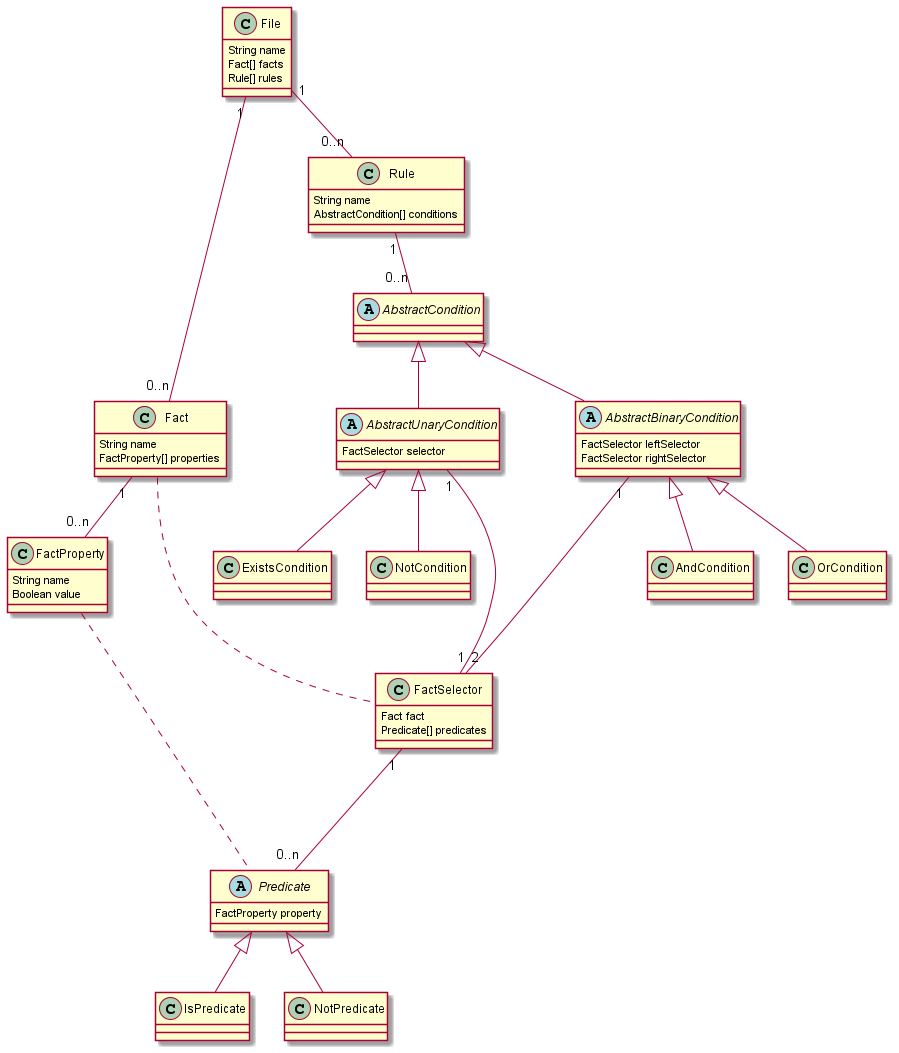
\includegraphics[width=0.95\textwidth]{Sections/images/ReallySimpleRuleLanguage.png}}
    \caption{RSR Concept Hierarchy}
    \label{fig:RSRDiagram}
\end{figure}

This design was then realised in MPS.
As the aim is to attempt different projections we did not initially optimise for editing.
The structure is as show in figure \ref{fig:RSRStructure} and the editors including those shown in figure \ref{fig:RSREditors}.

\begin{figure}
    \centering
    \begin{minipage}{0.30\textwidth}
        \centering
        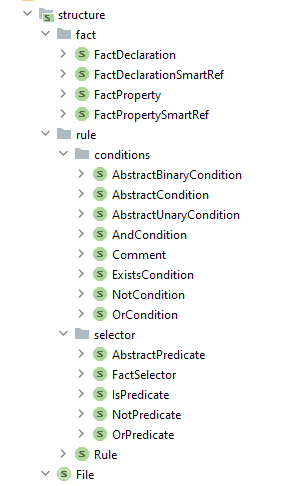
\includegraphics[width=0.9\textwidth]{Sections/images/RSRStructrure.png}
        \caption{RSR}
        \label{fig:RSRStructure}
    \end{minipage}\hfill
    \begin{minipage}{0.70\textwidth}
        \centering
        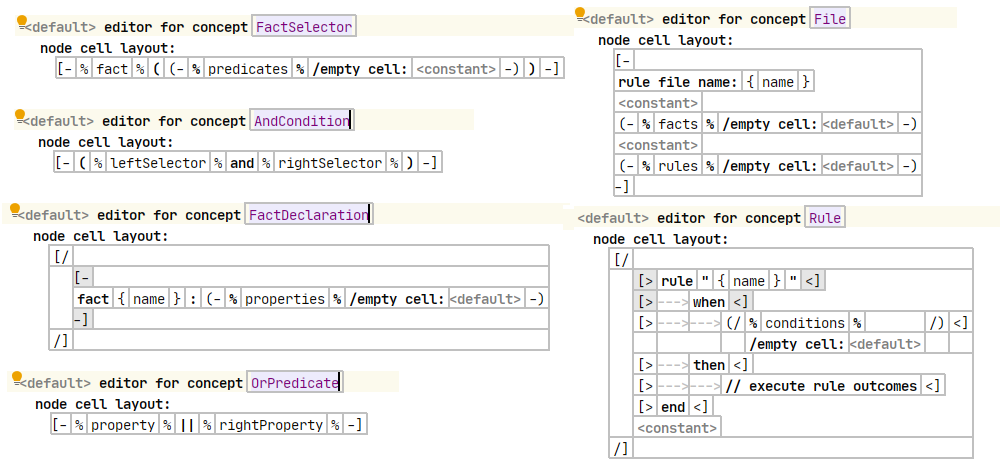
\includegraphics[width=0.9\textwidth]{Sections/images/RSREditors.png} 
        \caption{Editors}
        \label{fig:RSREditors}
    \end{minipage}
\end{figure}

Part of the research question is using projections to reason about large files.
In order to answer this we needed to simulate a large file.
To do this we had to enter a large number of rules.
As this becomes tedious we added a number of editing aids including substitute menus to speed up the entry of conditions, as shown in figure \ref{fig:RSRSubstituteMenu}.
This image, shows that before I had to select an ExistsCondition concept, and thereafter select the Fact for the condition.
After adding the substitute menu, I could immediate select the Fact I wanted and it would then automatically be wrapped with an ExistsCondition node. I could immediatly select the Fact and the 

\begin{figure}[h]
    \centering
    \fbox{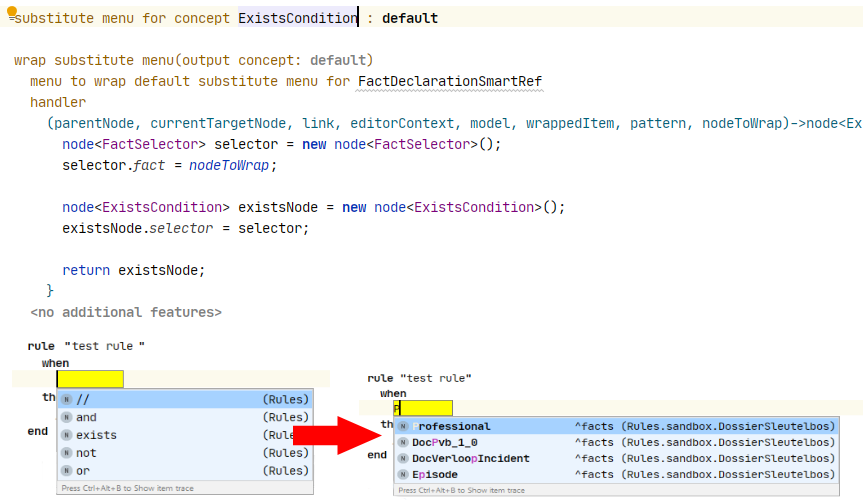
\includegraphics[width=0.95\textwidth]{Sections/images/RSRSubstituteMenu.png}}
    \caption{RSR Substitute Menu}
    \label{fig:RSRSubstituteMenu}
\end{figure}

We also added some intentions to invert incorrectly added conditions.

Finally, we added a constraint to scope the fact properties in predicates to the Fact chosen in the FactSelector.
This made it much easier to select properties in the predicates as indicated in figure \ref{fig:RSRConstraint}.
In the figure you can see that before the scoping constraint it showed a list with dozens of potential FactProperties, that represented all the FactProperties in the Model.
After the constraint is added it only shows the two properties associates with the Fact from the FactSelector.

\begin{figure}[h]
    \centering
    \fbox{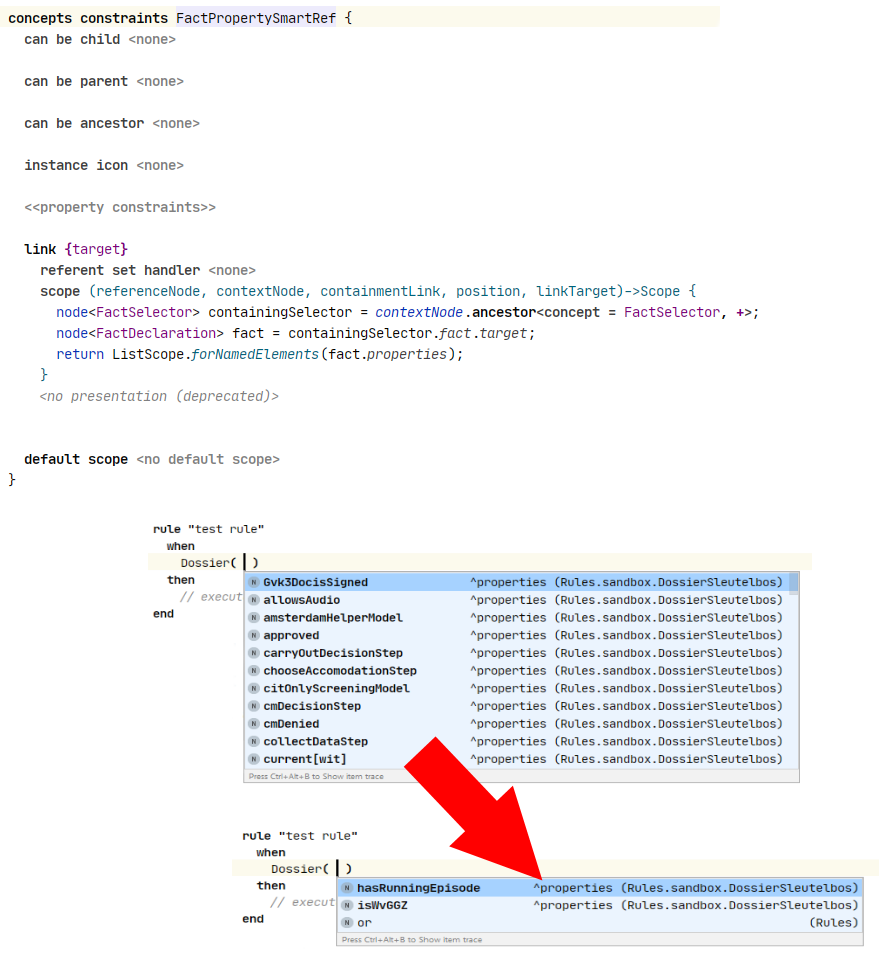
\includegraphics[width=0.95\textwidth]{Sections/images/RSRConstraint.png}}
    \caption{RSR Scoping Constraint}
    \label{fig:RSRConstraint}
\end{figure}

Thus, we have described the entire implementation of the Really Simple Rules Language.

After implementing the language we wrote a program with a large number of rules.
This program on which we will experiment with the different projections.
An example of our default Drools like text projection is show in figure \ref{fig:RSRProgram}.

\begin{figure}[h]
    \centering
    \fbox{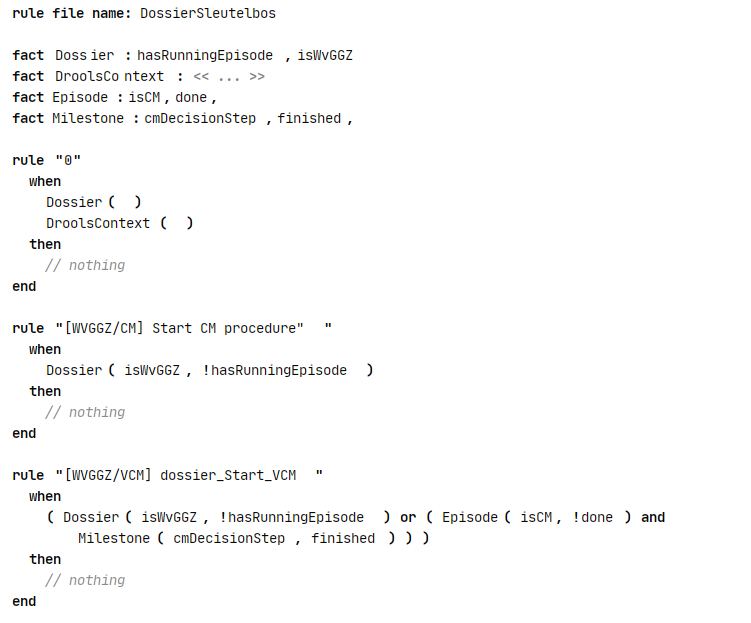
\includegraphics[width=0.95\textwidth]{Sections/images/RSRProgram.png}}
    \caption{RSR program}
    \label{fig:RSRProgram}
\end{figure}

The alternative projections will be discussed in the results section \ref{section:Results_ADR}.

\subsection{Drools-Lite Language}

The RSR was useful as an initial language, however is suffered two major Issues.
Firstly, it's limitations as a language were so great that it was not able to handle many necessary scenarios.
Secondly, our projections would have to be validated by developers with Drools experience.
For this reason we needed to create a projectional language that was much closer to the Drools language.

Our next Language, Drools-Lite, contains many more of the features of Drools.
The preliminary design is shown in figure \ref{fig:DroolsLiteDiagram}.


\begin{figure}[htbp]
    \centering
    \fbox{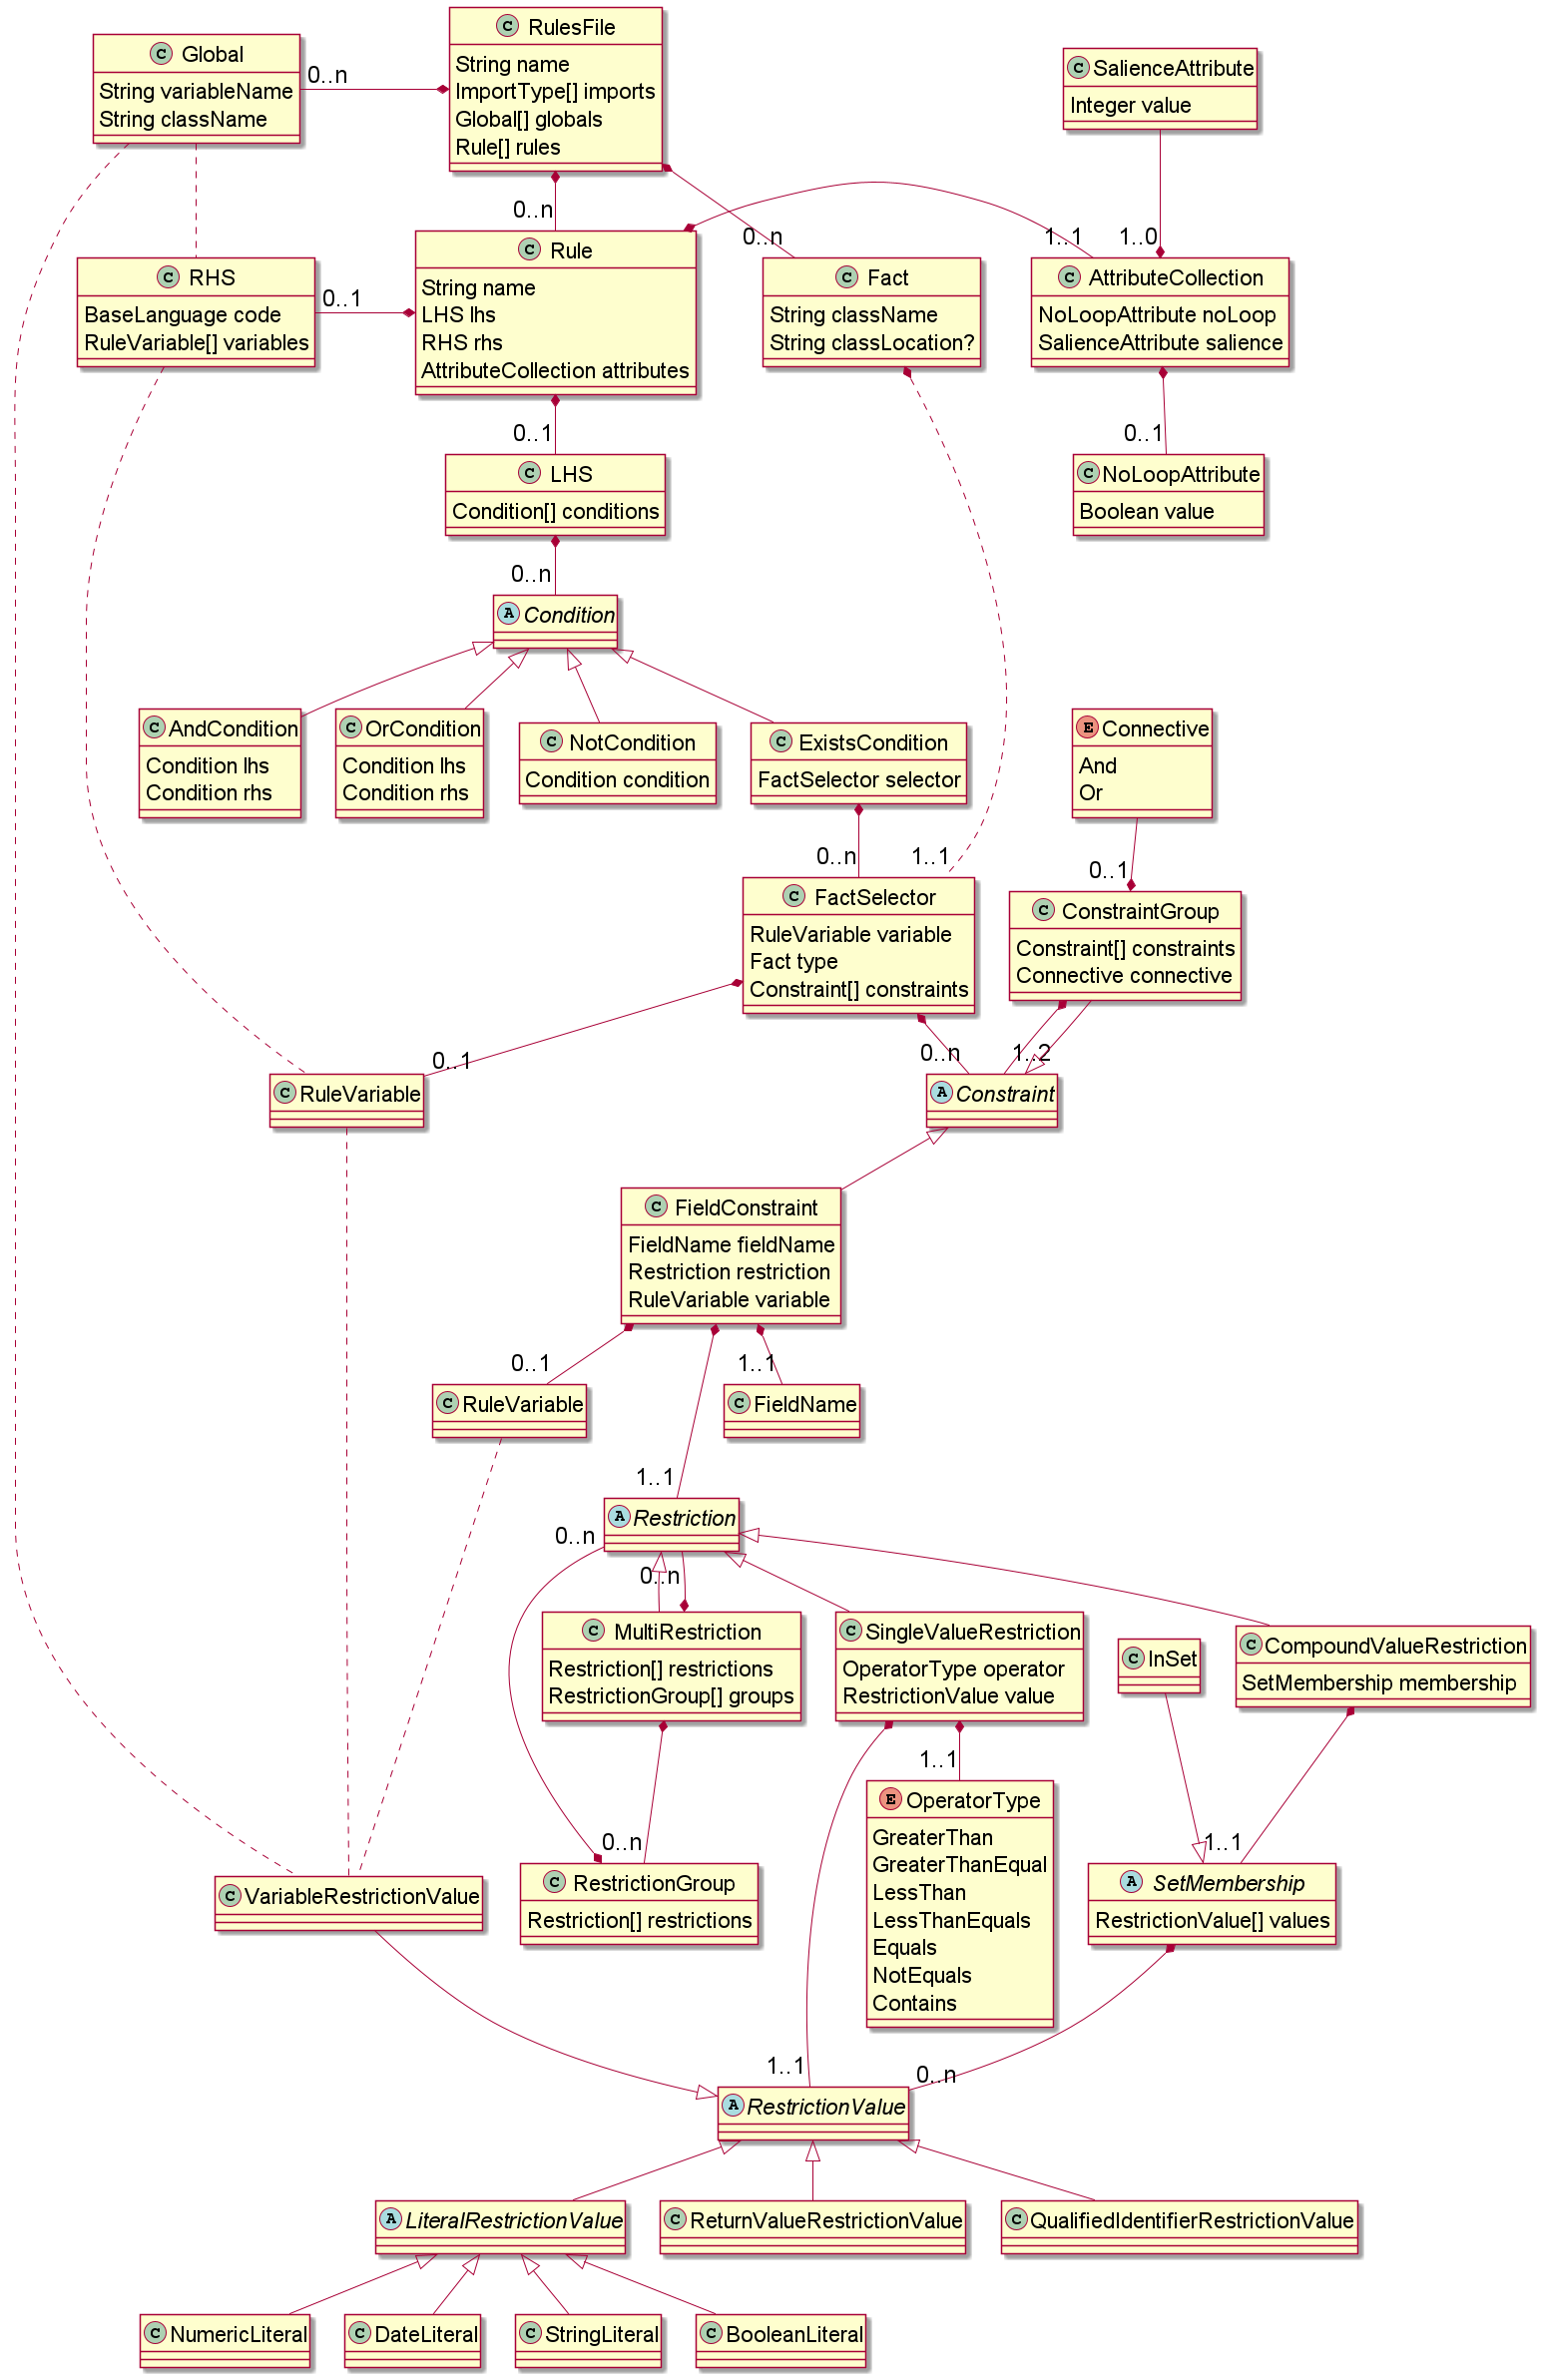
\includegraphics[width=0.85\textwidth]{Sections/images/DroolsLiteStructure.png}}
    \caption{Drools Lite Structure}
    \label{fig:DroolsLiteDiagram}
\end{figure}
\newpage
\section{Method: Survey}\label{section:Method_survey}
The validity of the the Prototype was tested using a survey.
If a survey is not well designed then it could lead to invalid or irrelevant outcomes.
As well as describing the design and procedure of the survey, we also outline any threats to its validity in this chapter.
Our choice of survey technique is a Questionnaire.

\subsection{Questionnaire Design}
The questionnaire can be found in appendix \ref{Appendix:Questionaire_text}.
To design the survey of our prototype, we followed a number of rules derived from the works of Bryman\cite{bryman2016social} and de Vaus\cite{de2013surveys}.

As advised, first we devised a clear introduction to describe the research.

We considered existing questions.
With regards to projectional editing, we requested the original questionnaires from three papers\cite{meacham2020adaptivevle,berger2016efficiency, voelter2014towards} pertaining to tools developed using projectional editing.
From these questionnaires we found [X] that we considered and decided against using any of them.

When formulating the questions we had the specific research question ``Which projections can help developers to get appropriate feedback about rules?'' in mind.

The pool of Drools users that we were personally in contact with was incredibly small.
Thus we had to rely on responses from strangers.
For this reason, we tried to make the questionnaire as quick to finish as possible.
This meant we looked particularly hard at removing questions that did not help us to our research goal.

We piloted the questionnaire with both ourselves and our industrial supervisor.

The instructions to each of the questions were tested for clarity, by a non-technical third party.

The only open question was one for which we wished to extract sentiment.
Rather than having yes/no questions, where appropriate we applied a Likert scale\cite{likert1932technique}.

The design of survey monkey layout makes sure that questions do not span pages.

The socio-demographic questions (skill level and experience) were left to the end and research based questions were toward at the beginning.

We took care to rework questions that were long, ambiguous, general, or leading to not be so.
We also took care to remove jargon, negative wording, and questions that asked about more than one thing.

\subsection{Participants}

The requirement for participants is that they have at least a little experience with using Drools.
It was our hope to get a statistically significant number of participants.

\subsection{Validity}
Non-response bias\cite{armstrong1977estimating} will be addressed by making the questionnaire short and easy to answer.
Because of the nature of the participant selection for this survey, it will be difficult to address the bias of self selection caused by voluntary response.

Common method bias, i.e. ``variance that is attributable to the measurement method rather than to the construct the measures represent''\cite{podsakoff2003common} can be responsible for 25\% or more of variable relational influence.
As we are only conducting a single survey, we won't be able to do much to prevent this, however we will take the following small precautions.
Testing the survey to remove question ambiguity, mood influences, and length issues.
Mixing the survey order of questions will be used to mitigate the issues caused by similarity of items, proximity of items, and location of items.
We will mitigate survey administration biases by administering some of these questionnaires manually and some online.
We will make sure that there are no right or wrong answers and aim toward fact based questions.
We will vary the scales of our Likert scales and the types of questions.

The main statistical methods to address this bias, i.e. ``Harman's single factor test''\cite{podsakoff2003common} and the``marker variable''\cite{lindell2001accounting} were found to be lacking in grounding\cite{gorrell2011countering}.
Marker variable is considered appropriate if used with caution.
With the size of our expected returns, it may not be possible to gain a statistically significant outcome.

\subsection{Pre-test}
The first attempt at the survey was sent to our industrial supervisor, who has experience with Drools.
We used this to remove ambiguously worded or leading questions and test that the length was truly between 5-10 minutes.
This lead to the following changes:
[TODO: add changes after we have tested]


\subsection{Sampling}
As within our own professional network we only had acquaintance with (6?) Drools developers, we had to expand our reach to those we did not personally know.

Our approach was first search StackOverflow for question askers and answerers on the subject of Drools.
Our preference was to find email addresses, failing that twitter contacts.
This proved to be quite limited, especially in attempting to get contact details, 13 email addresses and 6 twitter addresses.

Our next approach was to trawl our LinkedIn connections for anyone with drools as a proclaimed skill.
Whilst we had no one in our direct contacts, at one level of separation we found 204 connections.
From these we could extract 54 email addresses and 40 twitter addresses, with only a small crossover with the addresses harvested from StackOverflow.

We chose not to expand to third level contacts, as we thought this would be harder to sell as to why they should feel comfortable answering us.

\subsection{Procedure}

The questions, as described in appendix \ref{Appendix:Questionaire_text}, was uploaded to Survey monkey.

To encourage response, especially amongst only tangentially known participants, we crafted a short introduction, using techniques designed to enhance response as discussed by amongst others Cialdini\cite{goldstein2008yes}.
As seen in figure \ref{fig:persuasive_introduction}, the attics discussed by Cialdini, as signposted in table \ref{table:persuasive_introduction}.
\begin{table}[h]
    \begin{center}
        \begin{tabular}{ |l | l |  } 
            \hline
            Key &  Tactic\\
            \hline
            1  & Short option for those with no time \\
            2  & Credentials matter \\
            3  & Recognition, (this might backfire as I hardly remember any of my LinkedIn connections) \\
            4  & Consistency, they reported they have Drools experience, so they must live up to it \\
            5a\&b  & Social Proof - other people have already answered \\
            6  & showing value \\
            7  & Special because of scarcity \\
            8  & Labelling - ``I see you to be a good person'' \\
            9  & The word ``Because'' has an outweighed effect \\
            10 & Compliment Expertise \\
            11 & ``Every little helps'' \\
            12 & point out a fault \\
            13 & own the fault \\
            14 & ask a favour \\
            15 & add inconvenience \\
            16 & Rhyming \\
            17 & hand written note \\
            \hline
        \end{tabular}
    \end{center}
    \caption{persuasion tactics in figure \ref{fig:persuasive_introduction}}
    \label{table:persuasive_introduction}
\end{table}

\begin{figure}[h]
    \centering
    \fbox{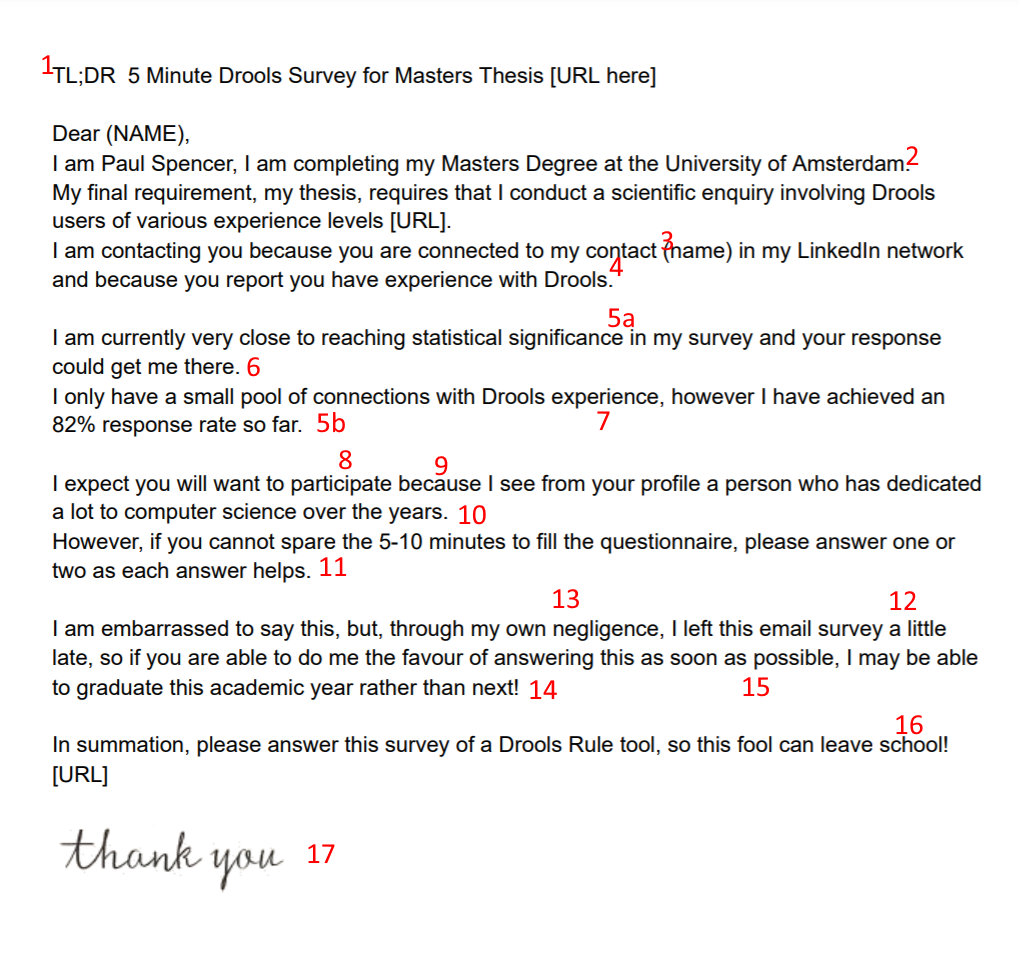
\includegraphics[width=0.85\textwidth]{Sections/images/persuasion.png}}
    \caption{persuasive introduction.}
    \label{fig:persuasive_introduction}
\end{figure}

These were sent to our list of drools using strangers and we sat back and awaited response.

    \chapter{Results}\label{chapter:Results}

\section{Results: Systematic Literature Review}
\label{section:Results_SLR}

We carried out a systematic literature review (SLR), as described in the methods section \ref{section:Method_systematic_review}.
We summarise the results of our SLR as ``undetermined''.
We make this statement because the review design was not wholly appropriate for the problem domain.

We could not find a quality assessment checklist that adequately dealt with action design research (ADR) studies.
This inadequacy proved problematic, as most of the primary studies were ADR studies.
Therefore, what follows should be considered the results of a quasi-SLR, with the quality assessment stage ignored.

\subsection{Papers Selected}
We logged the details of what we describe in this section in appendix \ref{Appendix:SLRLog}.

Figure \ref{fig:search_results} shows the results of the five iterations that the search went through.
Out of 173 results, we had 50 papers that initially seemed to pass our inclusion and exclusion criteria from our initial search.
From the initial 50, we added 18 papers from a possible 109 in our first iteration of forward and backwards snowballing.
The next snowballing iteration returned three papers that matched our criteria.
The third round of snowballing had no papers matching our criteria and thus terminated this stage of selection.

\begin{figure}[htbp]
    \centering
    \fbox{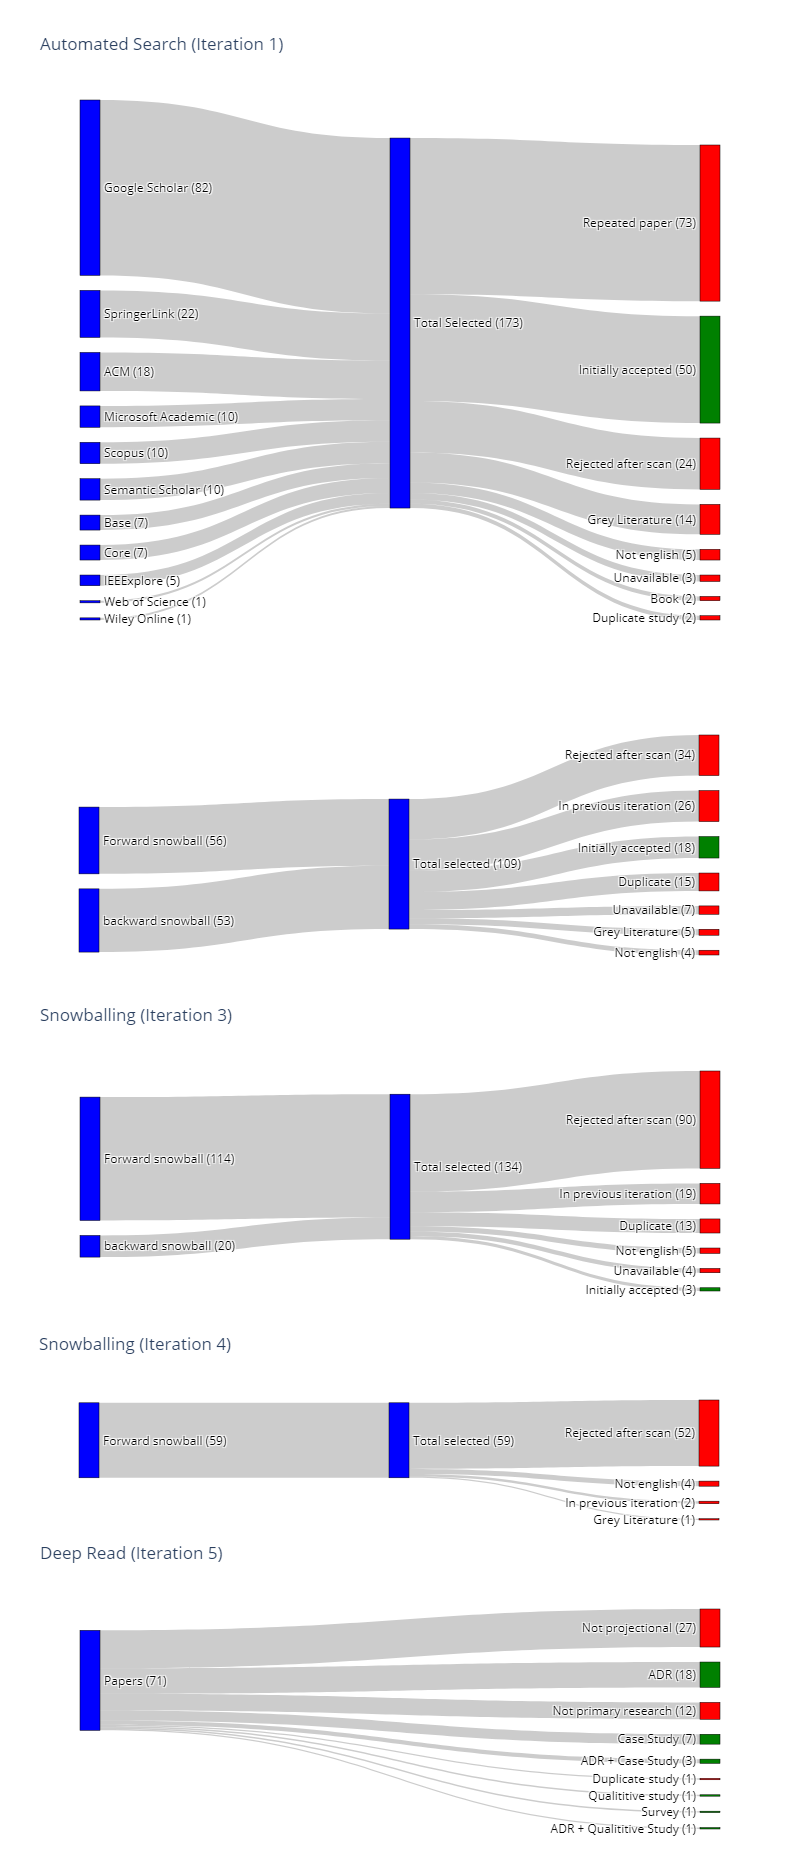
\includegraphics[width=0.75\textwidth]{/Sections/images/search_sankey.png}}
    \caption{Search results}
    \label{fig:search_results}
\end{figure}


Our final selection iteration involved a deeper scan of the remaining 71 papers.
In this stage, we rejected 12 papers that were not primary research and one paper which reported on an already represented study.
Further, we rejected twenty-seven papers that were, on closer reading, not about projectional editing.

This final selection filter left us with 31 papers before the quality assessment filter.

\subsubsection{Sensitivity and Precision}
As a curio, we reappropriated Zhang's\cite{Zhang_2011} ideas of sensitivity and precision and applied them to the search engines rather than search strings.
We calculate the values for sensitivity and precision of the search engines as follows:
\[
        sensitivity = \frac{\#\;retrieved\;relevant\;studies}{all\;relevant\;studies} \;100\%
\]

\[
        precision = \frac{\#\;retrieved\;relevant\;studies}{\#\;studies\;retrieved} \;100\%
\]

Table \ref{table:sensitivity_precision} show that Google Scholar had the highest sensitivity, returning 22 of the 31 chosen studies.
This sensitivity came at the cost of a considerable proportion of false positives.
Microsoft Academic and SpringerLink were the joint-most precise, with half of their search results ending up in the final roster.
With the second-highest count of documents, the second-highest sensitivity, and joint highest precision, SpringerLink would appear to be the best all-around search engine for this field.
However, these figures are skewed by several of their articles coming from a single collection specifically about projectional editing.

\begin{table}[h]
    \begin{center}
        \begin{tabular}{ | l | c | c | c | c |} 
            \hline
            Search engine/library     & original \# & selected \# & sensitivity & precision\\
            \hline
            \hline
            ACM                        & 18          & 3           & 10\%        &  16\%    \\
            BASE                       & 7           & 3           & 10\%        &  43\%    \\
            CORE                       & 7           & 1           &  3\%        &  14\%    \\
            Google Scholar             & 82          & 22          & 71\%        &  27\%    \\
            IEEExplores                & 5           & 2           &  6\%        &  40\%    \\
            Microsoft Academic         & 10          & 5           & 16\%        &  50\%    \\
            Science.gov                & 0           & 0           &  0\%        &   0\%    \\
            SCOPUS                     & 10          & 3           & 10\%        &  30\%    \\
            Semantic Scholar           & 10          & 4           & 13\%        &  40\%    \\
            SpringerLink               & 22          & 11          & 35\%        &  50\%    \\
            Wiley Online               & 1           & 0           &  0\%        &   0\%    \\
            Web of Science             & 1           & 0           &  0\%        &   0\%    \\
            \hline
        \end{tabular}
    \end{center}
    \caption{Search engine sensitivity and precision}
    \label{table:sensitivity_precision}
\end{table}


\subsection{Quality Assessment}
Using the quality assessment checklists developed by Crombie et al.\cite{crombie1997pocket}, shown in appendix \ref{appendix:QualityAssesmentChecklist}, we examined the remaining 31 papers, which on the surface represented 37 primary studies.

Unfortunately, there were no checklists for ADR studies.
We, unsuccessfully, searched for an appropriate quality assessment checklist for ADR studies.
We did not find a suitable checklist and did not consider ourselves suitably qualified to make one.
So, we used the quality assessment checklist for case studies to assess the ADR studies.

We used a rudimentary scoring system of +1 value for positive answers, 0 for undetermined, and -1 for negative answers.
We arbitrarily defined that any study with an overall score greater than 0 was high enough quality to be part of our final analysis.

Unfortunately, we only found 6 out of 37 studies of high enough quality to pass this filter with this scoring.
Thus, we had to choose between changing our scoring, only using these six studies, terminating the SLR or ignoring the QA findings.

Changing a method until it gave the desired answer seemed unscientific to us.
Six studies seemed too few to give an overview of a field.
Abandoning the SLA seemed the correct course of action.
However, as we still wanted an overview, we decided to take a different course.
We accept that what follows is no longer an SLA. 
We titled it a Quasi-SLA, which is like an SLA, which ignores the quality assessment results.

We could not reconcile that 84\% of studies were high-quality enough to appear in recognised scientific journals yet were not of high enough quality to pass our SLR QA stage.
After considering this disconnect, we found two significant threats to the validity of the Quality Assessment stage.
The first being that a single researcher with no previous experience executed the QA stage.
The second is that either case study checklists are inappropriate for ADR studies or that ADR studies are inappropriate for SLRs.


\subsection{Analysis}
After Identifying the primary studies, we extracted data.
Appendix \ref{appendix:DataExtraction} shows the extracted data.
Figure \ref{fig:study_types} shows that most of the primary studies in our review were ADR studies.

\begin{figure}[h]
    \centering
    \fbox{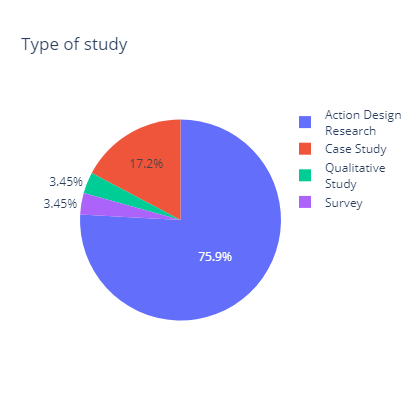
\includegraphics[width=0.35\textwidth]{/Sections/images/pie_study_type.png}}
    \caption{Study types}
    \label{fig:study_types}
\end{figure}

\subsubsection{Tools Used}
We split the studies to see which were to do with purely research projects and which were researching using already publicly available commercial or open-source products.
To calculate this, we removed one primary study, a survey, as it covered many tools and options, but none of which was in-depth.
The chart in figure \ref{fig:public_vs_research} shows that over 80\% of the projects were studying already existing publicly available options.

Of the publicly available software studies, we wanted to know which software attracted the most academic interest.
Figure \ref{fig:public_programs} shows that 74\% of the studies into projectional editing that used a publicly available product used JetBrains MPS.

\begin{figure}
    \centering
    \fbox{\begin{minipage}{0.47\textwidth}
            \centering
            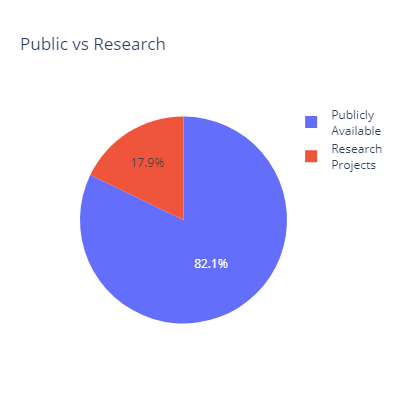
\includegraphics[width=0.85\textwidth]{Sections/images/pie_projectional_publicvsresearch.png}
            \caption{Public vs research}
            \label{fig:public_vs_research}
        \end{minipage}\hfill
        \begin{minipage}{0.53\textwidth}
            \centering
            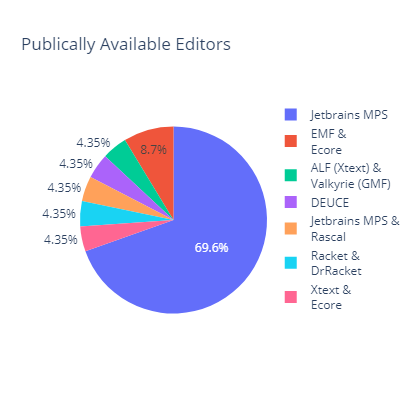
\includegraphics[width=0.85\textwidth]{Sections/images/pie_projectional_publicprograms.png} 
            \caption{Publicly available programs}
            \label{fig:public_programs}
        \end{minipage}
    }
\end{figure}

During this analysis, we discovered that two of the papers we had initially categorised as primary studies were, in fact, proposals, and thus we removed them from our analysis.

\subsubsection{Sentiment}

In this study, we included all 29 papers.
We tagged each section from those papers that talked about projectional editing.
We then broke each section into sentences and ran those sentences through a sentiment analyser as described in section \ref{section:dataExtraction}.
We show the outcome of this sentiment analysis in figure \ref{fig:sentiment_analysis}. 
The charts show the relationship between the positive, neutral, and negative sentiment outcomes.
On the y-axis, we have an Id for the papers examined. 
We show the keys linking the Ids to the paper names in table \ref{table:paper_key}.

The charts in the first column of figure \ref{fig:sentiment_analysis} show the absolute number of sentences analysed per paper partitioned by whether they returned negative, neutral, or positive sentiment results.
The charts in the second column show these as percentages so that the papers are comparable.
In the charts in the third column, we removed the neutral scores and calculated the percentage positive to negative.
The final chart column is an aid to make it easier to scan whether papers trended positive or negative.
If we found the papers to be equally positive and negative, we classified them as neutral.

Over the 29 papers, we scanned a total of 3003 sentences.
Four hundred thirty-five were analysed as being positive, 1953 neutral and 615 negative.
Hence, 14\% were positive, and 16\% were negative.

10 of the 29 papers were more positive than negative when discussing projectional editing, 16 more negative and three equally negative and positive.

In figure \ref{fig:sentiment_analysis2}, we attempt to separate out sentiment by product category.  
These categories being Research projects, MPS, and all the other used products.
We ignored the survey paper in this one as it covered all these types.

MPS dominates the sentences accounting for 17 (61\%) of the 28 papers and 2051 (73\%) of the 2791 sentences analysed.

\begin{figure}[h]
    \centering
    \fbox{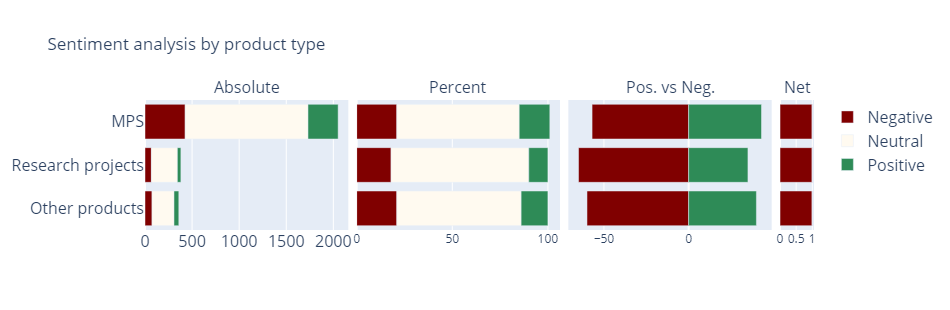
\includegraphics[width=0.95\textwidth]{/Sections/images/sentiment_analysis2.png}}
    \caption{Sentiment analysis by product}
    \label{fig:sentiment_analysis2}
\end{figure}

\begin{figure}[htbp]
    \centering
    \fbox{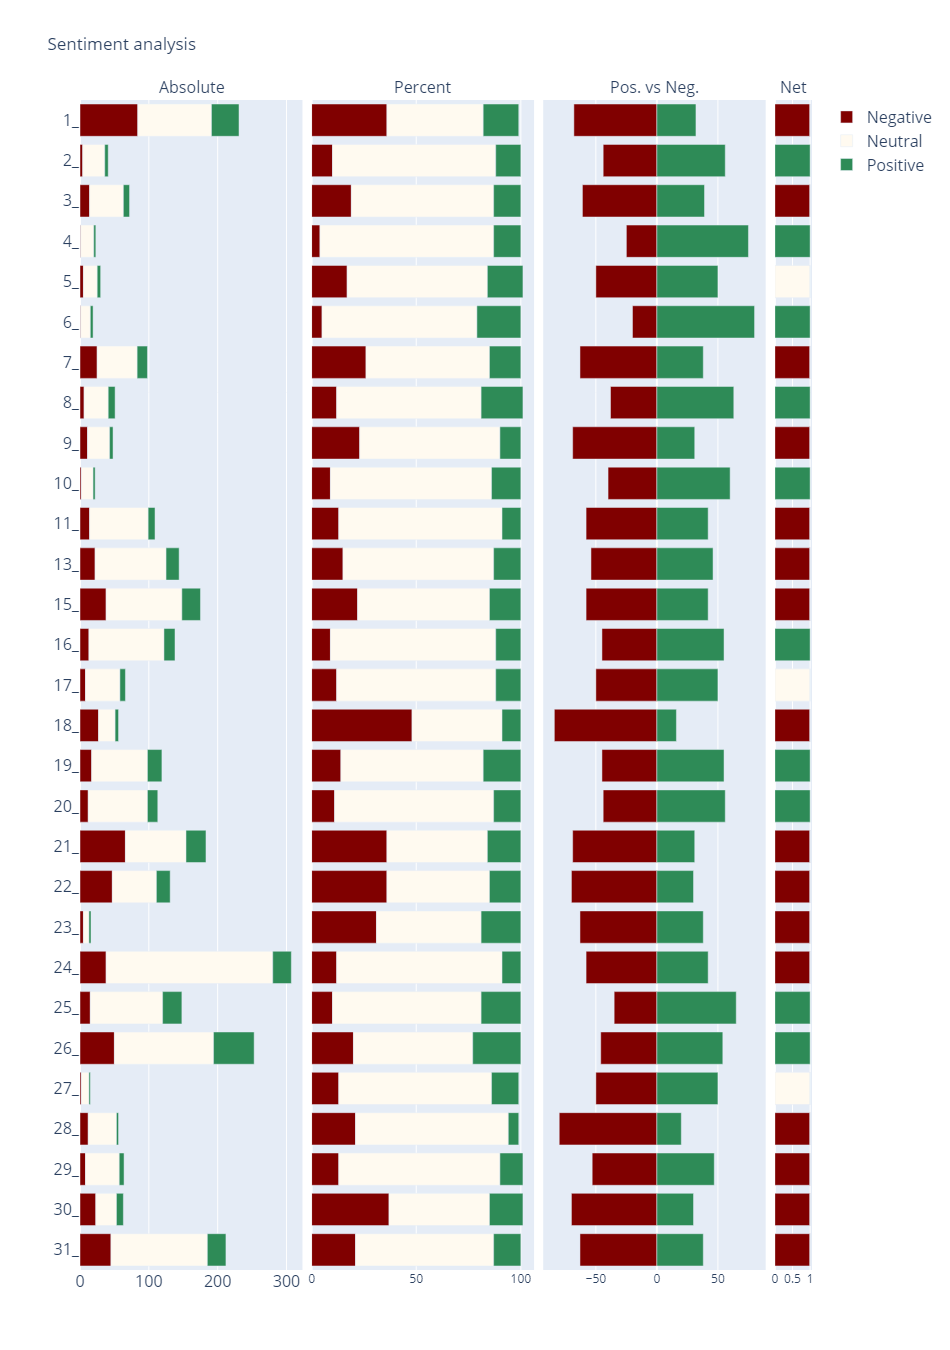
\includegraphics[width=0.95\textwidth]{/Sections/images/sentiment_analysis.png}}
    \caption{Sentiment analysis}
    \label{fig:sentiment_analysis}
\end{figure}


\begin{table}[htbp]
    \begin{center}
        \begin{tabular}{ |c  c|l | } 
            \hline
            Id  &                                        & Paper name                                                                  \\
            \hline
            1   &  \cite{voelterdomain_SLR}              & A domain-specific language for payroll calculations: A case study at DATEV  \\ \hline
            2   &  \cite{schropfer2021framework_SLR}     & A framework for projectional multi-variant model editors                    \\ \hline
            3   &  \cite{schropfer2020generic_SLR}       & A generic projectional editor for EMF models                                \\ \hline
            4   &  \cite{bucchiarone2019model_SLR}       & A model-driven approach towards automatic migration to microservices        \\ \hline
            5   &  \cite{meacham2020adaptivevle_SLR}     & AdaptiveVLE: An integrated framework for personalized online education      \\
                &                                        & using MPS JetBrains domain-specific modeling environment                    \\ \hline
            6   &  \cite{andersen2020adding_SLR}         & Adding interactive visual syntax to textual code                            \\ \hline
            7   &  \cite{addazi2021blended_SLR}          & Blended graphical and textual modelling for UML profiles: A                 \\
                &                                        & proof-of-concept implementation and experiment                              \\ \hline
            8   & \cite{meacham2020classification_SLR}   & Classification algorithms framework (CAF) to enable intelligent systems     \\
                &                                        & using JetBrains MPS domain-specific languages environment                   \\ \hline
            9   & \cite{furtado2021dsl_SLR}              & DSL based approach for building model-driven questionnaires                 \\ \hline
            10  & \cite{beckmann2020efficient_SLR}       & Efficient editing in a tree-oriented projectional editor                    \\ \hline
            11  & \cite{kolovos2020efficient_SLR}        & Efficient generation of graphical modelviews via lazy model-to-text         \\
                &                                        & transformation                                                              \\ \hline
            13  & \cite{bucchiarone2021engineering_SLR}  & Engineering gameful applications with MPS                                   \\ \hline
            15  & \cite{ratiu2021fasten_SLR}             & Fasten: An extensible platform to experiment with rigorous modeling of      \\
                &                                        & safety-critical systems                                                     \\ \hline
            16  & \cite{lafontant2020gentleman_SLR}      & Gentleman: A light-weight web-based projectional editor generator           \\ \hline
            17  & \cite{schropfer2019integrating_SLR}    & Integrating UML and ALF: An approach to overcome the code generation        \\
                &                                        & dilemma in model-driven software engineering                                \\ \hline
            18  & \cite{santos2020javardise_SLR}         & Javardise: A structured code editor for programming pedagogy in Java        \\ \hline
            19  & \cite{schindler2021jetbrains_SLR}      & JetBrains MPS as core DSL technology for developing professional digital    \\
                &                                        & printers                                                                    \\ \hline
            20  & \cite{simi2021learning_SLR}            & Learning data analysis with metaR                                           \\ \hline
            21  & \cite{stotz2021migrating_SLR}          & Migrating insurance calculation rule descriptions from Word to MPS          \\ \hline
            22  & \cite{munk2020model_SLR}               & Model-based safety assessment with sysml and component fault trees:         \\
                &                                        & Application and lessons learned                                             \\ \hline
            23  & \cite{bucchiarone2020papyrus_SLR}      & Papyrus for gamers, let’s play modeling                                     \\ \hline
            24  & \cite{merino2021projecting_SLR}        & Projecting textual languages                                                \\ \hline
            25  & \cite{cuinat2020specedit_SLR}          & SpecEdit: Projectional editing for TLA+ specifications                      \\ \hline
            26  & \cite{prinz2021teaching_SLR}           & Teaching language engineering using MPS                                     \\ \hline
            27  & \cite{barash2021teaching_SLR}          & Teaching MPS: Experiences from industry and academia                        \\ \hline
            28  & \cite{hempel2020tiny_SLR}              & Tiny structure editors for low, low prices! (generating guis from           \\
                &                                        & toString functions)                                                         \\ \hline
            29  & \cite{negm2020towards_SLR}             & Towards ontology-based domain specific language for internet of things      \\ \hline
            30  & \cite{lubin2020type_SLR}               & Type-directed program transformations for the working functional            \\
                &                                        & programmer                                                                  \\ \hline
            31  & \cite{ozkaya2021practitioners_SLR}     & What do practitioners expect from the meta-modeling tools? a survey         \\ \hline
        \end{tabular}
    \end{center}
    \caption{Paper key}
    \label{table:paper_key}
\end{table}

\subsubsection{A Narrative Synthesis}
Our synthesis of the papers that appear in table \ref{table:paper_key} will be short.
We will avoid rehashing the advantages and disadvantages of projectional editing, which come up again as we discussed these thoroughly in sections \ref{section:projectional_advantages} and \ref{section:projectional_disadvantages}.

Many of these papers focus on models and model-driven development, occasionally suggesting a shift towards textual modelling languages.
However, other papers point out that text does not always supply a suitable level of abstraction in modelling.
One paper suggested that developers prefer text, whereas maintainers and domain experts prefer visual projections, though this suggestion was unsourced.

When authors have used solutions other than MPS, they complain about issues such as MPS being heavyweight, with much overhead.
However, these authors then spend a great deal of time theorising about fixing issues in their architecture which, because of its architecture, MPS does not encounter.
These issues include synchronising between various views and how grammars deal with notations.

There is a fair bit of mention of a ``semi-projectional'' approach, which involves parsing at the leaf node level of the AST.
This approach is mainly from papers not using MPS, but also some which do.
The approach, it seems, is a reaction to the difficulty in simulating the text language experience in a projectional editor. 
It echoes the approach the Synthesizer Generator adopted when facing this same problem in the 80s.

The projects they describe are not in industrial use.
These authors suggest that projectional editing is probably best suited to helping novices learn a language. 

Those authors who use MPS are mostly discussing products developed for use in an industrial setting or how best to teach projectional editing to a broader audience.
MPS, when used, is often seen as a critical enabler.
Two of MPS' properties that garner the most mentions are the ease of composition and multiple views.

The users of MPS agree that simulating the experience of the text editor user in the projectional environment is still very hard.
However, new plug-ins are making this somewhat more manageable.
The most prominent carrion call amongst the MPS users is for a web-based interface.

The steep learning curve is another issue.
Several papers offer solutions to this, such as example-driven development, gamification, grammar to MPS plug-ins and something called a ``language wheel''.

In general, researchers using MPS have a few gripes with usability but seem to be very positive.
One paper, which was not using MPS, said that some problems become intractable when dealing with graphical models.
Another paper, in a coincidence of word use, when describing the decision to use MPS, explained that it was because it presented a tractable level of complexity. 

\newpage
\section{Results: Action Design Research}\label{section:Results_ADR}

\subsection{Really Simple Drools}

The Really Simple Drools Language (RSD) acted as a training ground for our new projections.

\subsubsection{Context-Aware Color Scheme}
After the default text projection, the first projection we made was giving the text a colour scheme.
This form or augmentation in IDEs is probably the most basic that we see.
Available in structured editors since the 1980s\cite{cowlishaw1987lexx}, syntax highlighting displays text in various colours and fonts according to the meaning of the terms.
Syntax highlighting is helpful for the comprehension of code, as least for small code bases\cite{sarkar2015impact}.

\begin{figure}
    \centering
    \fbox{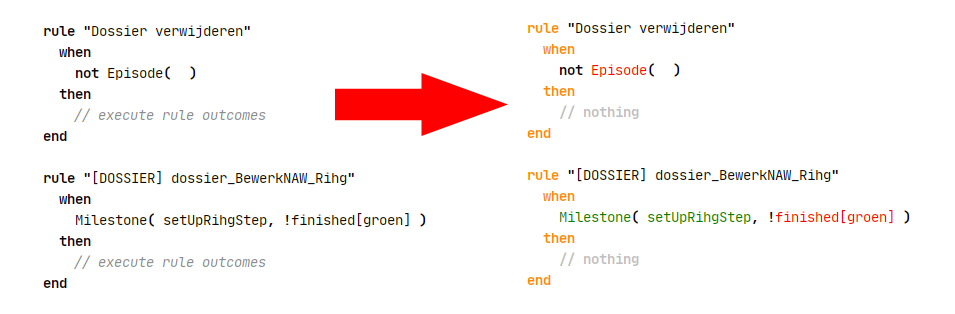
\includegraphics[width=0.99\textwidth]{Sections/images/coloredTextProjection.png}}
    \caption{Context aware color scheme}
    \label{fig:colorscheme}
\end{figure}

Developers at our host organisation use Eclipse or IntelliJ Community Editions to edit code, neither of which has syntax highlighting for Drools. Thus, the addition of this feature would immediately benefit them.
However, IntelliJ IDEA, the paid version, already provides this feature for Drools.
We extended the colour scheme to indicate whether the selection is looking for a positive or negative match to offer another visual augmentation that we considered valuable.
Figure \ref{fig:colorscheme} shows this projection.

\texttt{Facts} contained by \texttt{NotConditions} and \texttt{FactProperties} that are part of a \texttt{NotPredicate} appear highlighted in Red.
\texttt{ExistConditions} and \texttt{IsPredicates} have their content coloured green.
We did not test whether this improved understanding.

\begin{figure}
    \centering
    \fbox{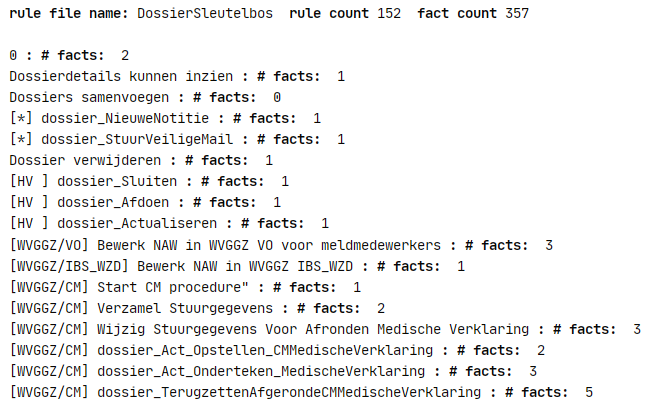
\includegraphics[width=0.75\textwidth]{Sections/images/summaryProjection.png}}
    \caption{Summary projection}
    \label{fig:summaryProjection}
\end{figure}

\subsubsection{Summary Projection}
Our next projection allows developers to have a quick overview of the \texttt{Rules} and complexity of those \texttt{Rules}.
Figure \ref{fig:summaryProjection} shows that the developers can get an overview of both the number of \texttt{Rules} and the number of \texttt{Facts} in each of the \texttt{Rules}.

The building of this projection only required adjusting two editors.
The \texttt{Rule} count and \texttt{Fact} count were added to the \texttt{Fil}e editor using Read-Only Model Access to count the descendants of the \texttt{File} that are \texttt{Rules} and \texttt{Facts}.
The \texttt{Rule} editor was adjusted only to show the \texttt{Rule}'s title and, again using the model access, the count of the descendants of the \texttt{Rule} that were \texttt{Facts}.

Whilst this may look like a report that any language workbench could create, the \texttt{File} name and the names of the \texttt{Rules} are editable in this projection.

\subsubsection{Filtering}
Whilst investigating how to handle extensive collections of rules, we looked to domains that already handle extensive collections of items.
The domain of data analysis has a long history of handling large volumes.
Among their two most used tools for exploration are sorting and filtering.

The nature of business rules lends them to some projectional options that would not make sense with other programming styles.
Because of the independent nature of the rules, filtering lends itself to the business rules style.
The semantic meaning of the order of business rules means we did not find a good use case for sorting rules.
So, we decided to implement a filtering projection.

Whilst use of filtering occurs in other places in the coding pipeline, such as deciding on what code completion to present\cite{hou2010towards} and version control visualisation\cite{yoon2013visualization}, we were unable to find any research on applying filtering directly to code files.
Consequently, we think what we present here is an original idea.

\texttt{Rules} that use the same \texttt{Facts} or \texttt{FactProperties} are likely to be related.
Thus, these seemed the obvious items to filter.
We created a projection where if the developer filtered by a \texttt{Fact} or a \texttt{FactProperty}, the projection would filter out all rules that did not contain the item.
Once the rules were filtered, the projection only shows \texttt{Facts} and \texttt{FactProperties} used by those \texttt{Rules}.

\begin{sidewaysfigure}
    \centering
    \fbox{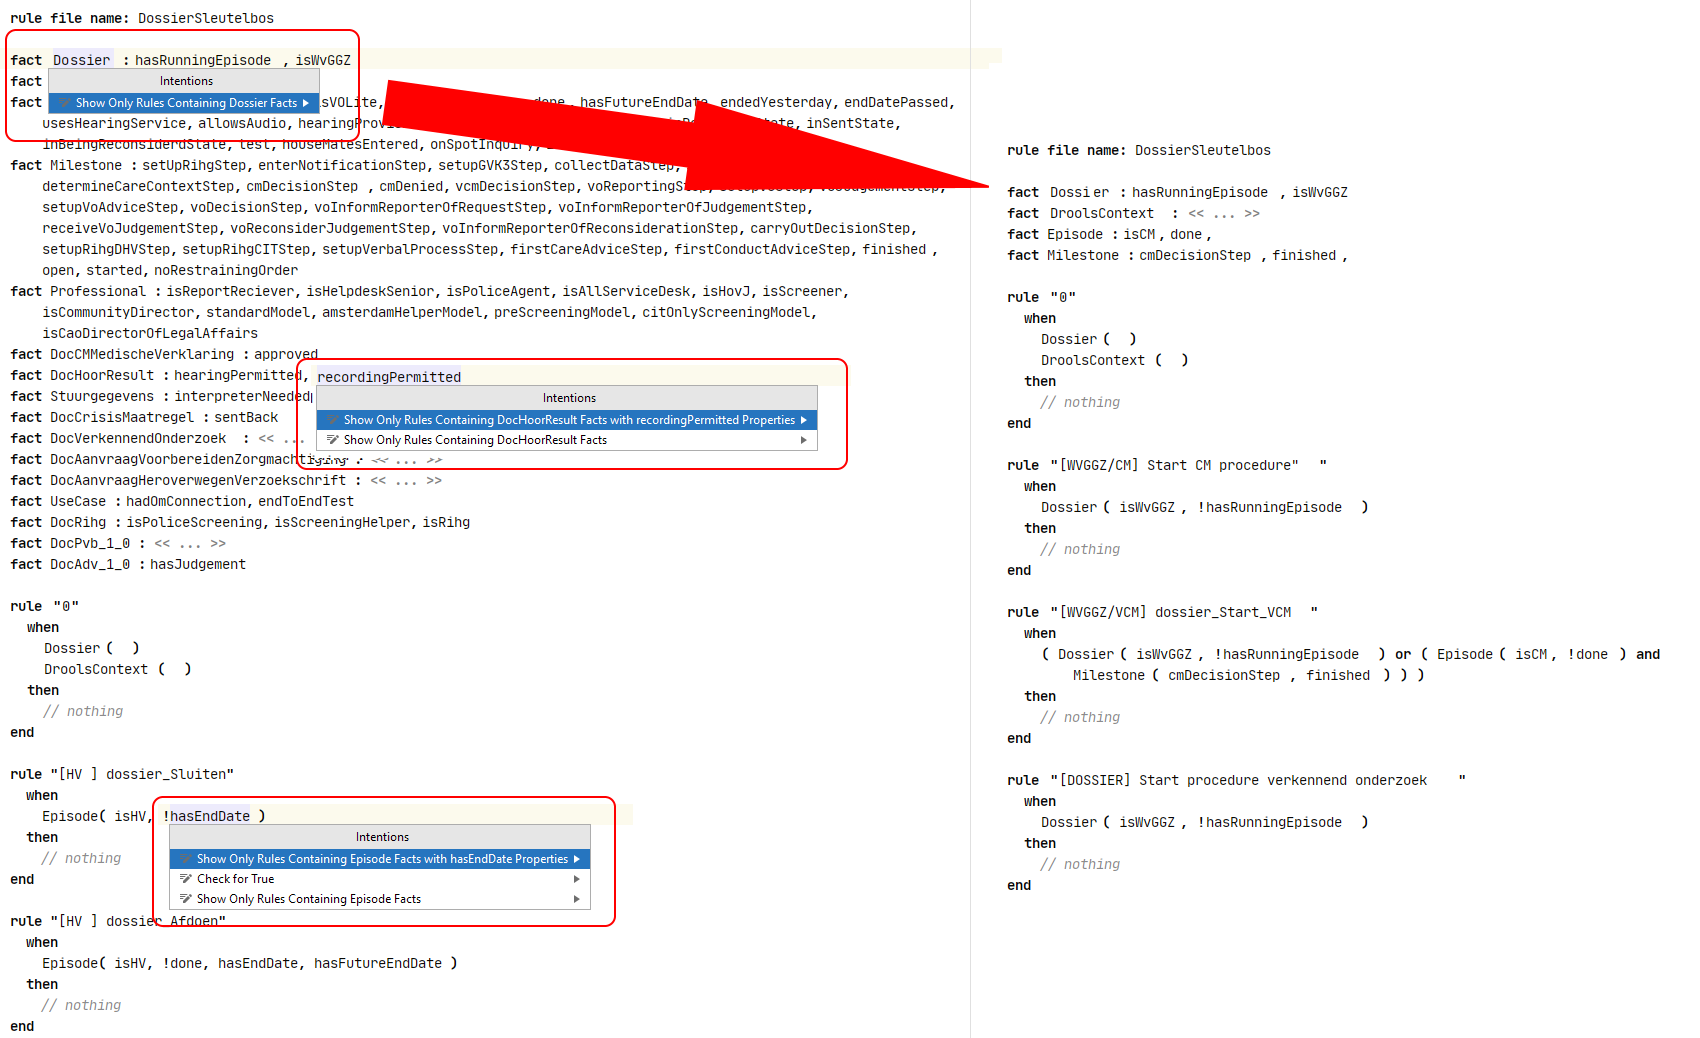
\includegraphics[width=0.99\textwidth]{Sections/images/filteringProjection.png}}
    \caption{Filtering projection}
    \label{fig:filteringProjection}
\end{sidewaysfigure}

In our implementation, shown in figure \ref{fig:filteringProjection}, we show three places where we use intentions to filter the code.
The first is an intention associated with a \texttt{Fact}.
We show the outcome of choosing this filter on the righthand side of figure \ref{fig:filteringProjection}.
The second intention is on a \texttt{FactProperty}.
As the \texttt{FactProperty} is a child of a \texttt{Fact}, we see both intentions.
The third highlighted intention is on a \texttt{FactProperty} Reference.
It also shows an intention associated with a \texttt{FactReference} in the \texttt{FactSelector} that holds the \texttt{FactPropertyReference} as a child.

One of our guidelines was, as much as possible, to build our projections as separate languages, non-invasively extending RSD.
In our first approach at the filtering, we failed on this count by invasively adding properties to \texttt{Fact} and \texttt{FactProperty} Concepts of the RSD to determine whether they were visible.

Our following approach created subclasses of \texttt{Fact}, \texttt{FactProperty} and \texttt{File}.
This approach, however, requires running a macro on the code file to migrate \texttt{Facts}, \texttt{FactProperties} and \texttt{Files} to \texttt{FilteredFacts}, \texttt{FilteredFactProperties}, and \texttt{FilteredFiles}.
This migration means that the \texttt{FilteredFile} could now only be used by languages that extend our new filtered language.

Our final approach was to add a \texttt{Filter} Concept, reference the filtered nodes, and have the editors make the visibility calculations based on this singleton node.
Whilst more complex, this removed the need for invasive changes and allowed other languages to combine with the filtering language.

Filtering is a handy projection.
However, it breaks Dijkstra's rule ``the purpose of abstraction is not to be vague but to create a new semantic level in which one can be absolutely precise.''\cite{dijkstra1972humble}.
This projection fails this rule by hiding some of the meaning of the code.
This projection has no way of containing the whole code whilst a filter is applied.
However, we feel that so long as there is a clear indication that a filter is applied, then we see this as a tool in a similar vein to the code collapsing functionality found in most modern-day editors.

\subsubsection{Table}
Thus far, our projections have been textual ones that other non-projectional language workbenches could implement.
Creating a table was our first non-parseable projection.

We choose the table projection based on the observations of Miller\cite{miller1956magical} about the number of items people can retain in their memory.
This observation leads us to conclude that the fewer essential items that are off the screen and, therefore, in the developers' memory, the better.

\begin{sidewaysfigure}
    \centering
    \fbox{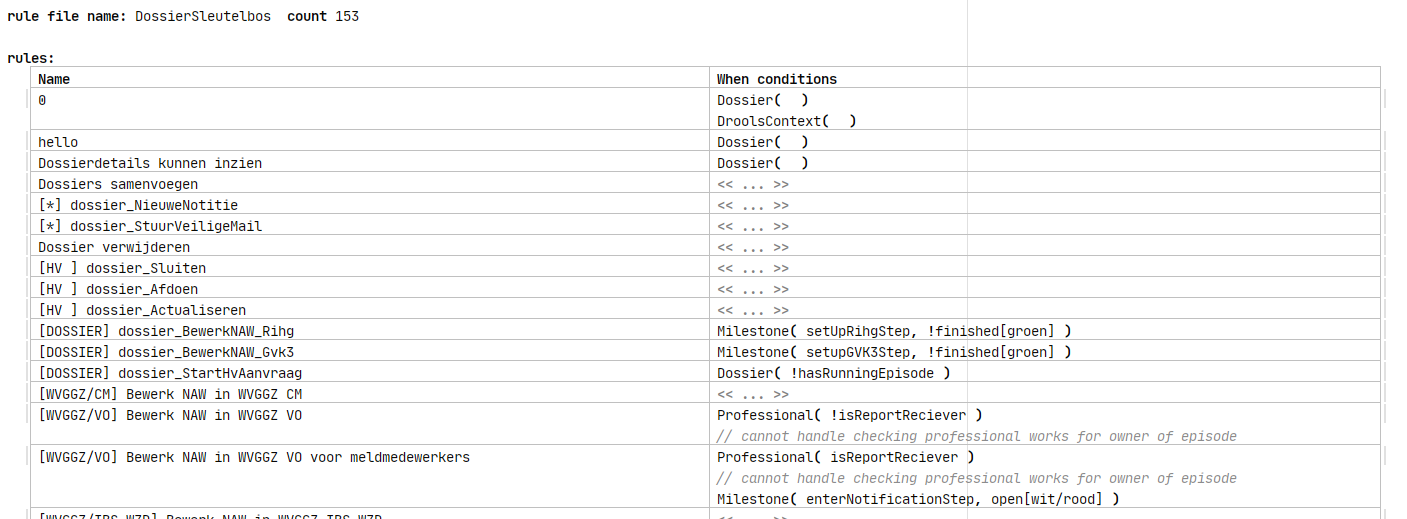
\includegraphics[width=0.99\textwidth]{Sections/images/tableProjection1.png}}
    \caption{Table projection}
    \label{fig:tableProjection1}
\end{sidewaysfigure}

Figure \ref{fig:tableProjection1} shows our rudimentary first table.
This simple table has only the \texttt{name} property and the \texttt{when} children of the \texttt{Rules} in the \texttt{File}.
We implemented this projection using the tables extension in the MPS-Extension plug-in, created by Sascha Lißon.

\subsubsection{Cross-tab}
Our next tabular projection is a cross-tab inspired by a decision table.
The idea behind this projection is that the previous table does not give any visual queues as to how \texttt{Rules} are related.
With a cross-tab, one can easily see which \texttt{Rules} are using the same \texttt{Facts}.

\begin{sidewaysfigure}
    \centering
    \fbox{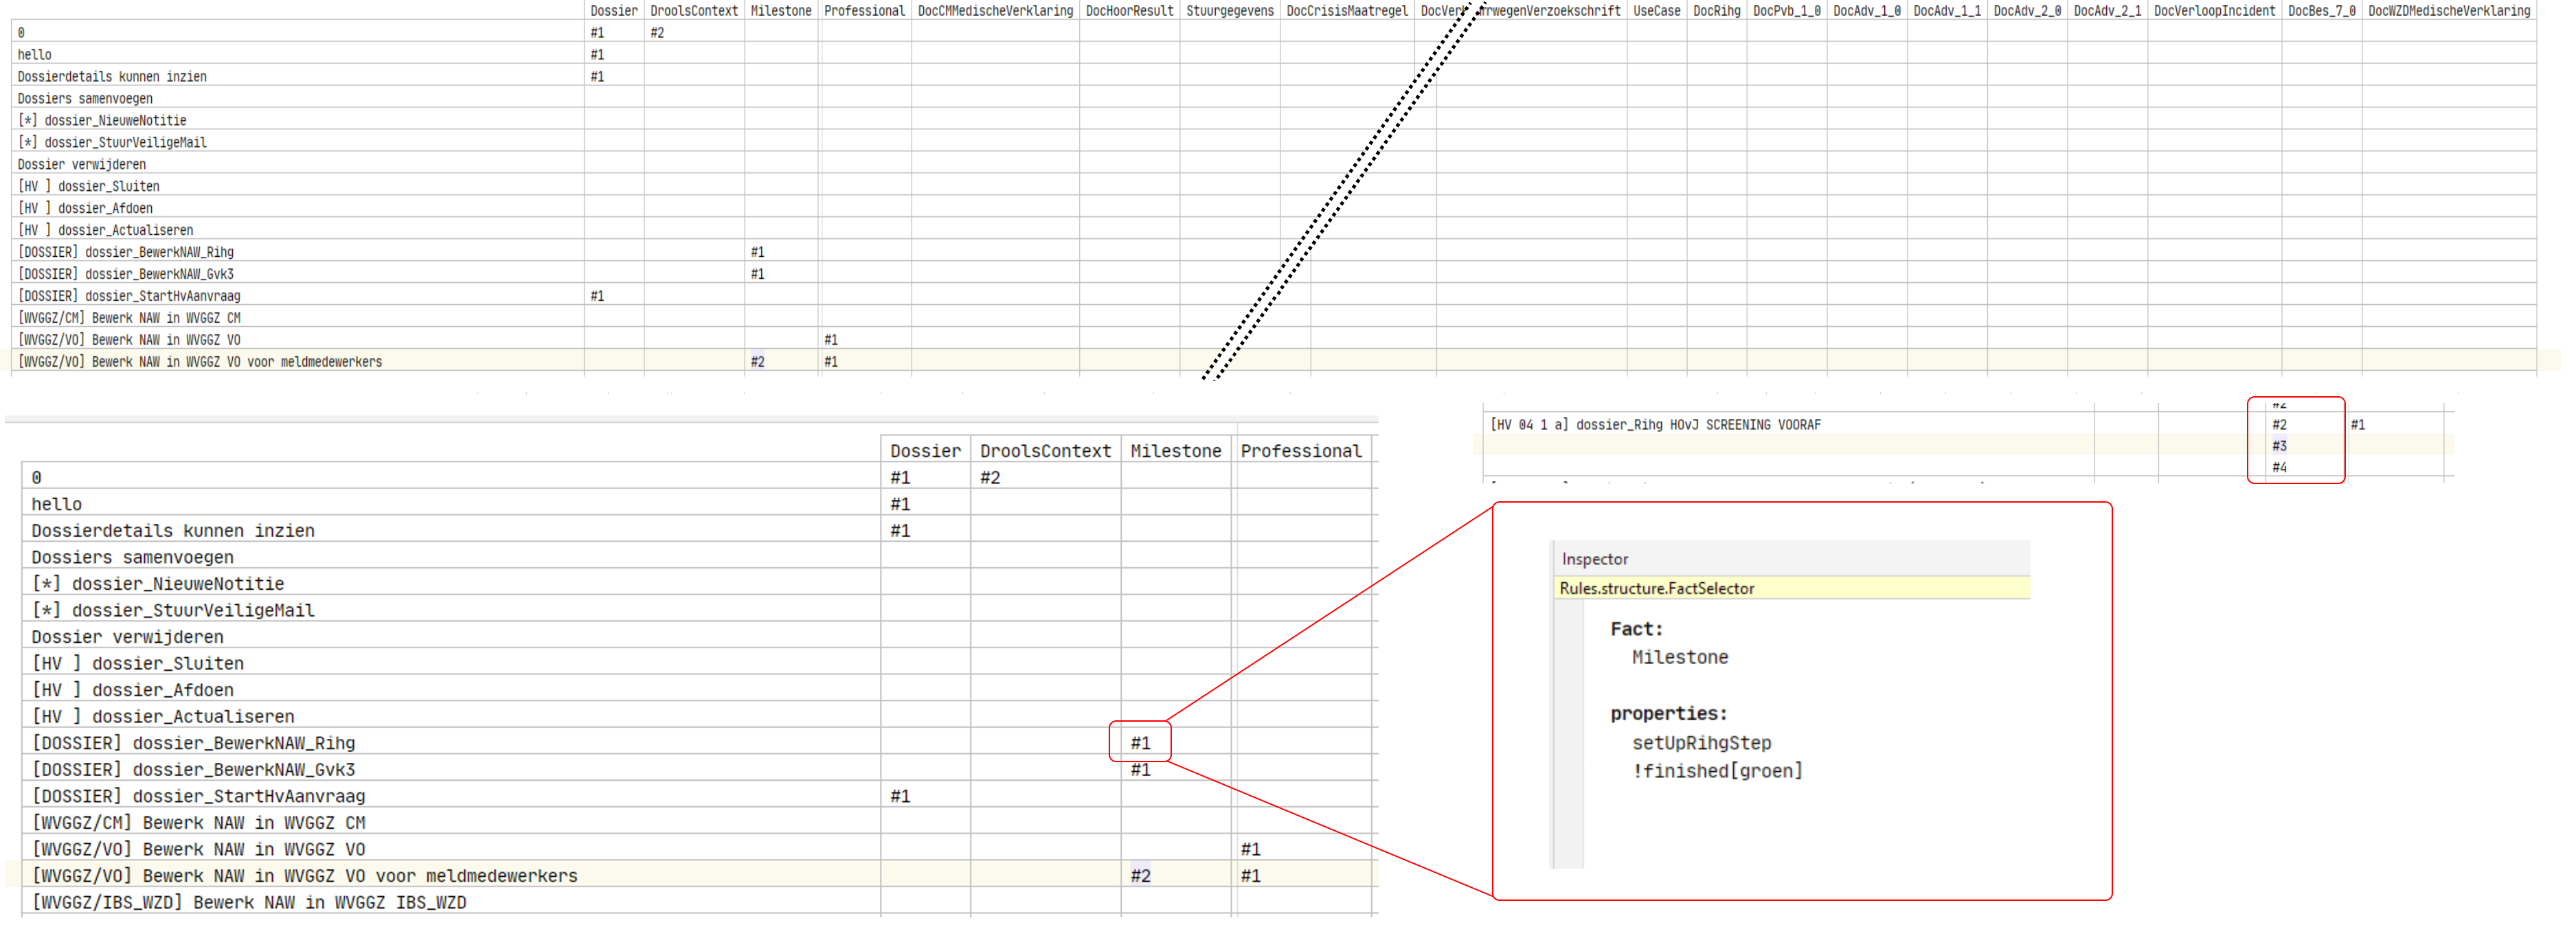
\includegraphics[width=0.99\textwidth]{Sections/images/crosstabProjection1.png}}
    \caption{Cross-tab projection}
    \label{fig:crosstabProjection1}
\end{sidewaysfigure}

Figure \ref{fig:crosstabProjection1} shows our implementation of the cross-tab.
At the top, we can see an immediate problem with a cross-tab, and that is if we have the whole \texttt{File} included, the table will be very sparse.
Figure \ref{fig:crosstabProjection1} also has a close-up of a cell showing a \texttt{Rule} using three \texttt{FactSelectors} that reference the same \texttt{Fact}.
The other close-up shows that all the details of the selected \texttt{Fact} are available in the inspector.

The sparse table will not be a problem if the columns are thin enough to keep the table in a single screen's width.

\begin{sidewaysfigure}
    \centering
    \fbox{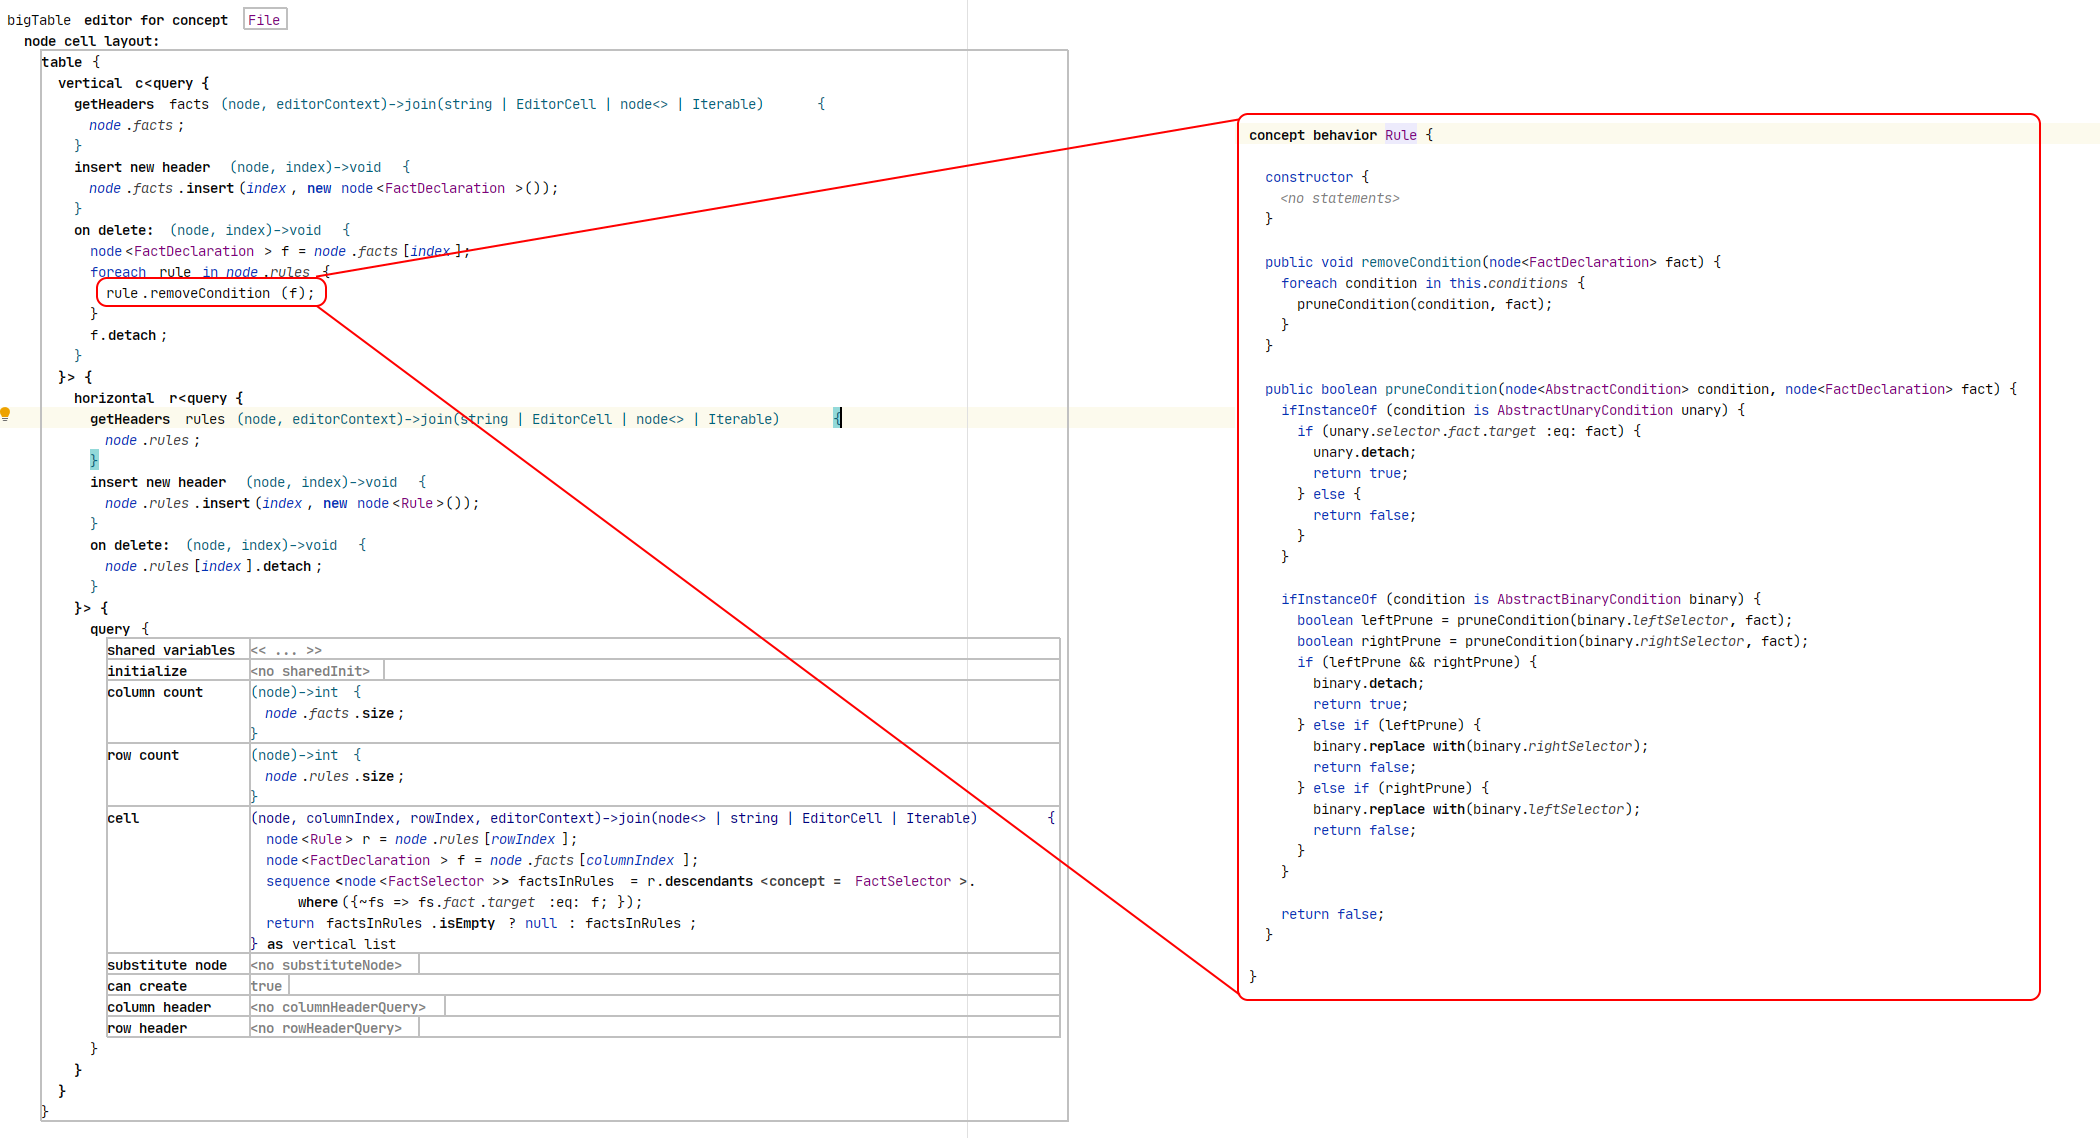
\includegraphics[width=0.99\textwidth]{Sections/images/tableDeleteCode.png}}
    \caption{Table Fact deletion code}
    \label{fig:tableFactDeletion}
\end{sidewaysfigure}

Everything is editable in this table, including deleting a \texttt{Fact} from a \texttt{Rule}.
The table plug-in and MPS enabled most of the editing in the projection by default.
An extra editing feature we added to this table was the ability to delete a \texttt{Fact} from the \texttt{File} by deleting a \texttt{Fact} column, and in the process also deleting all references to the \texttt{Fact} from all the \texttt{Rules} in the \texttt{File}.
The code shown in figure \ref{fig:tableFactDeletion} shows how we can walk the trees in each \texttt{Rule} to delete unary conditions and convert the non-deleted side of binary conditions into unary conditions to allow this \texttt{Fact} deletion.

Here we end our experiments in the RSD language.

\subsection{Drools-Lite}

Our subsequent experiments were with projections with the Drools-Lite language.
As described in section \ref{section:DroolsLite}, Drools-Lite is an implementation that is much closer to the complete Drools language.
This realism will allow us to create projections that we can present to experienced Drools developers for evaluation.

Of the learnings from the RSD language, one we felt needed fixing to improve understanding was the sparseness of the tables.
By implementing the principle of maximising cohesion, we discovered we could reduce the sparseness issue.
Therefore, as a precursor to our projections, we extended Drools-Lite with a new language that contained one structural item, the \texttt{RuleCollection}.
The \texttt{RuleCollection} is a child of the \texttt{File} and holds a collection of \texttt{Rules}.
The idea behind this is that related Rules can be placed in the \texttt{RuleCollection} to make it easier to examine them together.
This language also added an editor for the \texttt{RuleCollection} and intentions to move rules in and out of groups.

\subsubsection{Decision Table}

As the Drools language is analogous to a series of if-then statements, then perhaps its best visual equivalent is the decision table.
Decision tables are a ``powerful aid in programming, documentation, and in effective man-to-man and man-to-machine communications''\cite{pooch1974translation}.

\begin{figure}
    \centering
    \fbox{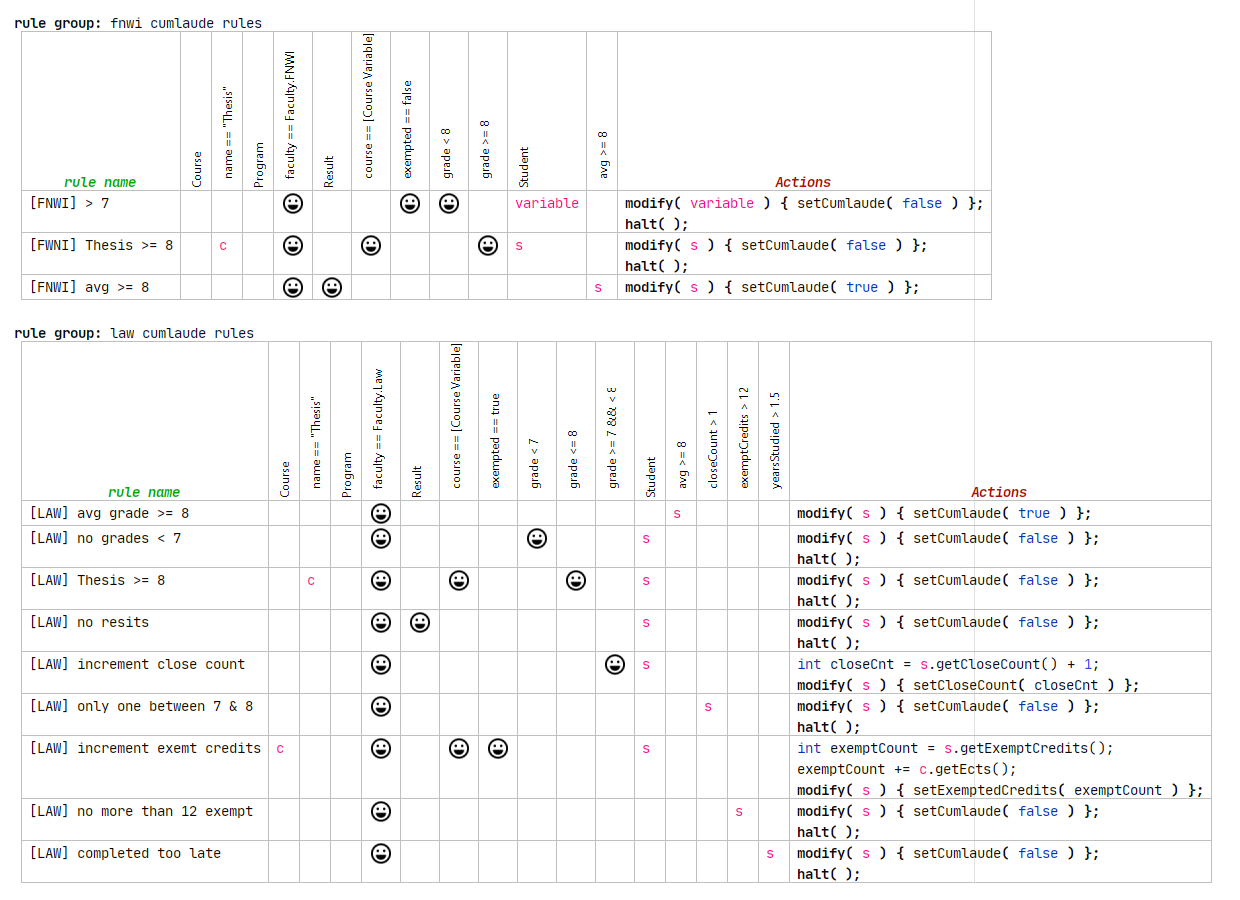
\includegraphics[width=0.99\textwidth]{Sections/images/decisionTableProjection.png}}
    \caption{Decision table projection}
    \label{fig:decisionTableProjection}
\end{figure}

We designed our table, shown in figure \ref{fig:decisionTableProjection}, to include some of the lessons learned from the RSD cross-tab that shown in figure \ref{fig:crosstabProjection1}.
The RSD language taught us that wasting visual real estate exacerbates sparseness issues in tables.
In the cross-tab table, horizontal scrolling is necessary, in part due to the column widths.
The columns were wide because the name of the \texttt{Fact} was displayed horizontally.

The Drools-Lite language allows for much longer selection criteria on \texttt{FactProperties}, which would lead to much wider columns.
Our solution was to develop a vertically orientated header cell and to use indentation to indicate if the cell is referring to just the \texttt{Fact} or a \texttt{Fact} and \texttt{FactProperty} combination.

Because this projection presents both the left and right-hand side of the rules, we had to handle the Concept that spans both - the \texttt{RuleVariable}.
We had to find a way to represent a \texttt{RuleVariable} that can be bound and used on the LHS and used on the RHS.
We achieved this by referencing a \texttt{RuleVariable} name in the cell representing the \texttt{Fact} or \texttt{FactProperty} to which it is bound.
With \texttt{RuleVariables} now being represented in the cells, we could no longer represent the cell being selected with an ``X'', as this could be confused with a \texttt{RuleVariable} name.
Projectional editing does not require communication of meaning through parseable ASCII text.
Thus, we decided to represent \texttt{Fact} selection with an image.
For arbitrary reasons, we chose a smiley face as that indicator.

The \texttt{Rule} names and actions are editable through the default functionality of the MPS extension.
We use intentions to add the selection of a \texttt{Fact} or \texttt{FactProperty} to a \texttt{Rule}.
We also use intentions for binding \texttt{RuleVariables}.

The major drawback of this design is that editing a rule with an as yet non-existent selection criteria became very clunky.
If the \texttt{Rule} we wished to edit already existed in the table, we had to use an intention to extract it from the group, change the criteria and place it back in.
At this point, the table would automatically adjust the column headings.

Experts examined this design in the questionnaire.

\subsubsection{SpreadSheet}

The domain-specific language for the finance world is the spreadsheet.
One study estimated that 90\% of computers had a spreadsheet on them\cite{bradley2009using}.
Dan Bricklin's VisiCalc drove personal computers into the office.
VisiCalc was succeeded by Lotus 1-2-3, which Microsoft Excel then succeeded as the dominant spreadsheet program in the workplace.

\begin{sidewaysfigure}
    \centering
    \fbox{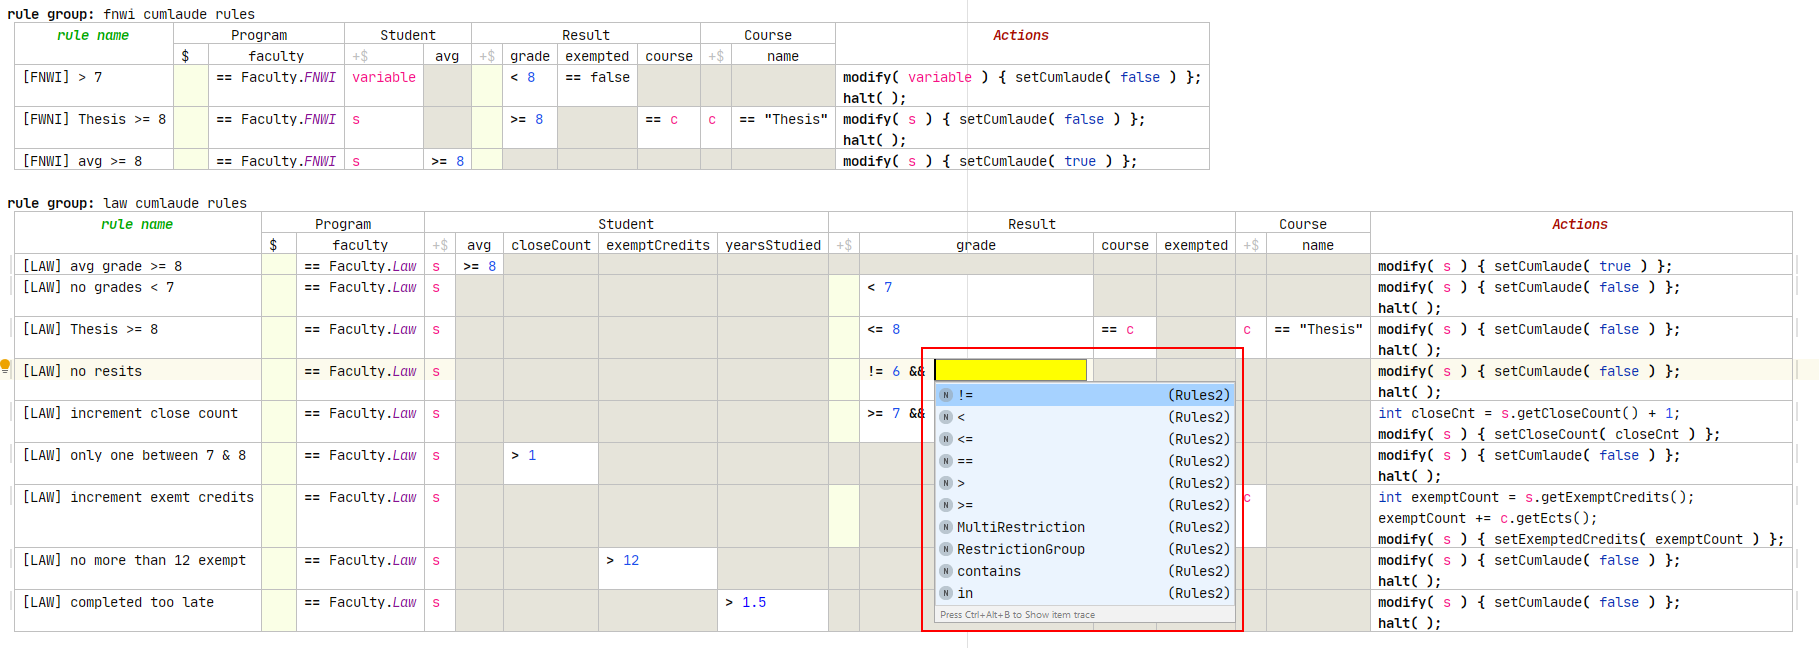
\includegraphics[width=0.99\textwidth]{Sections/images/SpreadsheetProjection.png}}
    \caption{Spreadsheet projection}
    \label{fig:SpreadsheetProjection}
\end{sidewaysfigure}

This level of familiarity with a paradigm led us to design a projection that had the look and feel of an Excel spreadsheet.
We show this design in figure \ref{fig:SpreadsheetProjection}.
To this end, we created a design where the selection criteria could be directly edited in the cell, as highlighted in the figure.


\begin{figure}
    \centering
    \fbox{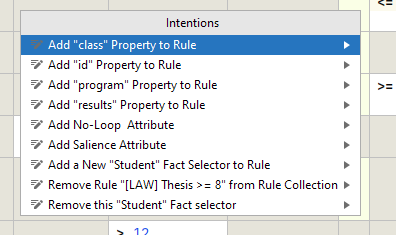
\includegraphics[width=0.95\textwidth]{Sections/images/spreadsheetIntentions.png}}
    \caption{Intention}
    \label{fig:SpreadsheetIntentions}
\end{figure}

\begin{figure}
    \centering
    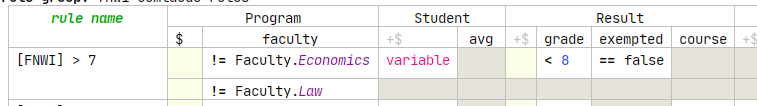
\includegraphics[width=0.95\textwidth]{Sections/images/spreadsheetTwoProperties.png} 
    \caption{Two of same property}
    \label{fig:TwoProperties}
\end{figure}


Each row is a \texttt{Rule} in this design, and each column is for a \texttt{RuleVariable} or a \texttt{FactProperty}.
If a property is selected, then the selection criterion is in the appropriate cell.
A grey/beige colour indicates unselected cells.
The RHS of the \texttt{Rule} appears in the actions column.
Adding as yet unused \texttt{Facts} or \texttt{FactProperties}, or removing existing ones, can be achieved with intentions, as shown in figure \ref{fig:SpreadsheetIntentions}.

This design also allowed us to have more than one selector for the same \texttt{FactProperty}, essential for our host organisation's code.
We demonstrate this in figure \ref{fig:TwoProperties}.

Experts examined this design in the questionnaire.

Here we end our experiments in the Drools-Lite language.

\subsection{Wireframe}

After brainstorming several ideas to present as wireframes to experts as possible projectional aids to understanding, we chose two.
We discuss them briefly in this section.

\subsubsection{Truth Table}
We decided to produce a truth-table wireframe example as we had had personal experience building truth tables to confirm the validity of Drools rules in our work.

The truth table seemed apt for the LHS of the Drools rule as, in essence, it is a boolean function.
Wittgenstein popularised the truth table in the Tractatus Logico-Philosophicus\cite{wittgenstein2013tractatus}.
They are so widely used in mathematics and computer science that we do not need to explain their use further.
Because of the combinatorial explosive nature of truth tables, with 2\textsuperscript{n} possible combinations, we would limit the display to a max of 6 \texttt{FactSelectors} and only show the paths that lead to the RHS execution.

\begin{figure}
    \centering
    \fbox{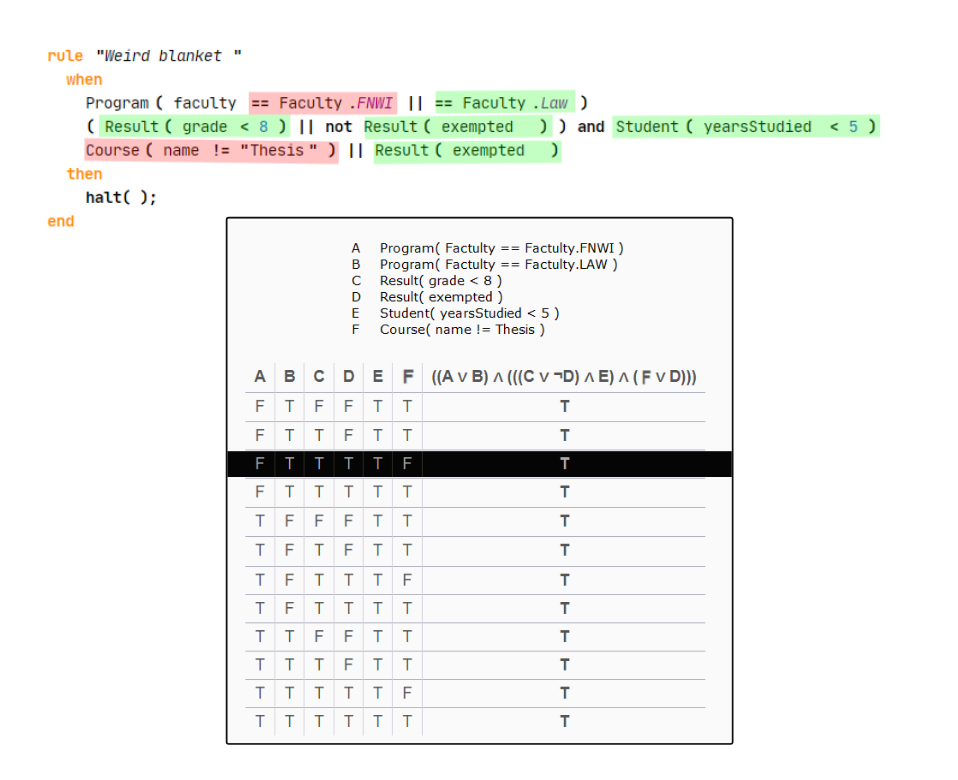
\includegraphics[width=0.80\textwidth]{Sections/images/truthtable.png}}
    \caption{Truth table projection}
    \label{fig:TruthTableProjection}
\end{figure}

Figure \ref{fig:TruthTableProjection} shows how we designed this to look.
The user experience would be that the \texttt{Rule} is selected, and the developer presses the up and down arrow keys to step through the different true (highlighted in green) and false (highlighted in red) \texttt{FactSelectors} that result in the \texttt{Rule}'s selection.

We presented this design to our experts to be validated.

\subsubsection{Circuit Diagram}
In our final projection design, we wanted to present a part of projectional editing that we had heretofore only made minimal use of.
That is the use of manipulatable graphics that can change the AST.

\begin{figure}
    \centering
    \fbox{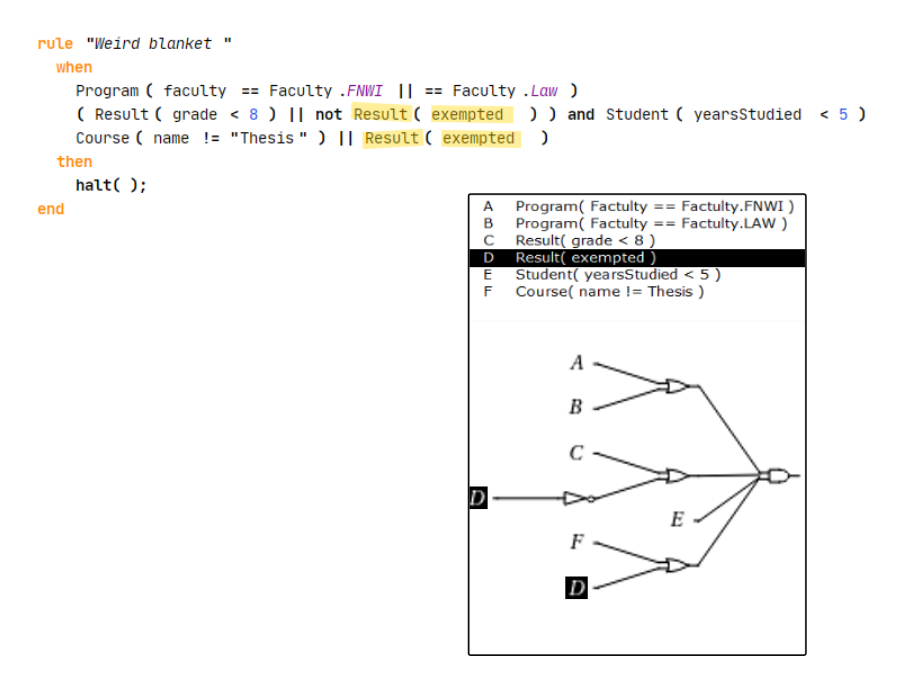
\includegraphics[width=0.80\textwidth]{Sections/images/CircuitDiagram.png}}
    \caption{Circuit diagram projection}
    \label{fig:CircuitDiagramProjection}
\end{figure}

We chose a logic circuit. 
The logic circuit represents a boolean operation as NOT, OR, XOR and AND Gates, with their inputs and outputs being inputs to other gates.
In our design, shown in figure \ref{fig:CircuitDiagramProjection}, the input wires to the gates are the \texttt{Facts} or \texttt{FactProperties} referenced in the LHS.

The user experience is that once the \texttt{Rule} is selected, the developer, by pressing the up and down arrow keys, can step through the different \texttt{FactSelectors} (highlighted in yellow) and shown in the circuit diagram, thus showing how the \texttt{Facts} relate to each other.

We present this design in the questionnaire for validation.


\newpage
\section{Results: Survey}\label{section:Results_Survey}


    \chapter{Discussion}\label{chapter:Discussion}

\section{Threats to Validity}  

\subsection{Construct Validity}


\subsection{Internal Validity}

\subsection{External Validity}

\subsection{Reliability}

\subsection{Repeatability vs Reproducibility}

\subsection{Method improvement}

    \chapter{Related Work}
\label{chapter:RelatedWork}

We split related work into three sections. 
Firstly, those relating to the state of projectional editing.
Next, those that address the understandability of business rules.
Finally, work on interesting projections.

\section{The State of Projectional Editing Workbenches}

Whilst we were particularly looking into the current state of projectional editing, there have been previous studies.
The language workbench challenges, which ran from 2011 to 2016, inspired many papers, most notably Erdweg et al.'s summaries of the 2013\cite{erdweg2013state} and 2015\cite{erdweg2015evaluating} challenges.
These papers looked into the capabilities of LWBs, including projectional LWBs.
Whilst these were interesting from the point of view of capabilities of LWBs. 
They did not touch on market penetration or other usage indicators, and thus the experimental workbenches were lined up equally against the well used.
Schindler et al.\cite{schindler2016language} looked at the experience of the language workbench challenge from the point of view of a projectional editing LWB, namely MPS.
This paper addressed the areas where projectional editing LWBs had a significant advantage over the other LWBs. 
We feel it is a shame that the LWB challenge is no longer occurring.

There does not seem to be much analysis of what is going on in projectional editing at the moment, except when there is an intersection with adjacent fields such as Model-Driven Approaches, Low-code, Language Orientated Programming, or language workbenches.
We found one systematic mapping study of LWBs\cite{iung2020systematic} from 2020 that again looked at the entire field of LWBs, including the projectional ones.
Whilst looking at LWB features, it also extended into areas such as domains of use.

With regards to MPS in particular, while there is no mapping of the state of the usage, we saw that papers earlier in the last decade tended to concentrate on how to improve the experience of using MPS, prototypes or new products, for example, \cite{pavletic2013extensible,voelter2014generic,voelter2015using,voelter2010language2,voelter2013mbeddr,voelter2013requirements,voelter2014projecting,voelter2015towards,voelter2010embedded,voelter2011product,ratiu2012implementing}.
Today, research involving MPS tends to be maturing into industrial use of the product and using it in teaching, e.g. \cite{prinz2021teaching,voelterdomain_SLR, schindler2021jetbrains_SLR,simi2021learning_SLR,barash2021teaching_SLR,stotz2021migrating_SLR,ratiu2021use}.

\section{Understandability of Business Rules}

A different approach to ours was taken in the VODRE project\cite{lapaev2014vodre}.
In place of visualising how the rules belonged together, it visualised how they were executed.
In optical design, they showed the execution paths that the expert systems used in coming to their conclusions.

In a similar fashion to the Drools DMN, Ostermayer et al.\cite{ostermayer2013simplifying} attempt the generation of rules using templating and an external editor.
Along the same lines, the G-AMC tool\cite{sa2016g} created a front end for developing rules.
However, in this case, in the domain of access control management.
These both face the issues we were trying to overcome by separating the tool and the language. 
They also focus on the generation of rules rather than the understanding of them.

\section{Interesting Projections}
Some of the most interesting projections are happening in industrial environments, and there are limited papers about these.
For example, Klaus Birk\cite{Birken_Interactive} uses the graphical modelling extensions for hierarchical component models in systems architectures, as well as getting live simulator responses to changes in the code.
Tom Beadman\cite{Beadman_Journey}, as a part of his tool Pasta, generates an interactive visual state machine to, for example, decide whether to check for fraud. 

Florian Bock's tool, stiEF\cite{Bock_stief}, is a language that uses a live update of graphical driving scenarios in the IDE.
Whilst this is not a two-way projection, a developer cannot interact with the visual scenarios.
However, it is a great feedback tool to let the developer know that they have correctly programmed their scenario. 
    \chapter{Conclusion}\label{chapter:Conclusion}

In this master's project we dove into the current state of projectional editing and presented and had verified a number of projections for the purpose of improving the understanding of Business Rules.
We conducted a systematic literature review (SLR), creates prototypes and conducted a survey of the impact they may have.
Through the SLR we examined the current state of projectional editing, finding it dominated by a single product.
We implemented the Drools language in MPS and through our prototypes we demonstrated some of the possibilities projectional editing can bring.
The results of our survey failed to confirm that these projections would bring the benefits we had hypothesised.

In this paper we described our work with first translating the Drools DSL into a projectional language followed by our explorations of projections.
We discussed the advantages and disadvantages of the different projections we created and analysed experienced developers reactions to them.

In this last section of this paper will return to the initial questions we were trying to answer from section \ref{section:Research_Questions}.
We will summarise the findings of our research and the contributions our work had made.
Finally we will discuss items that were out of scope for this project, but would give future research opportunities.

\section{Research Summary}
Our main research question, ``How can projectional editors and DSLs be combined to address feedback mechanisms for developers in the context of reasoning about rules in a rule-based business engine?'', motivated us to explore the field of projectional editing in this project.
This drove us to investigate if this field was worth investigating and, if so, how we can use existing tools to answer this.

\subsubsection{Research Question 1: ``What is the current state of language workbenches supporting projectional editing?''}
In this paper we presented an SLR which looked into the current state of projectional editing.
This SLR found that currently LWBs for projectional editing is a very narrow field, dominated by one product, JetBrains MPS.
Studies using products other than MPS spend time and effort discussing how to solve issues already solved in MPS.
Studies using MPS tend to be focused on products for industrial use or how to use MPS as a tool to teach Meta-Programming.
One area MPS is a little behind is the need for a web based development environment, both for the Language engineer, but especially for the developer.

A monoculture can be a risk.
Whilst there are many advantages to projectional editing, having only one successful product and supplier feels a little unhealthy.
On the other hand, the number of users of the tool is growing, as evidenced by the papers representing new projects in multiple industries, from hardware, through automotive industry, to Finance.

To conclude, the state of the projectional editing market, whilst niche, is maturing but with a current product monoculture.

\subsubsection{Research Question 2: ``Which projections can help developers get appropriate feedback about rules?''}

In our research we were able to develop a number of projections.  
This success was in large part facilitated by the flexibility and extensibility of the MPS tool which presented the ability to develop and extend DSLs very efficiently.

We presented two of the projections to experienced Drools users, along with two wireframes of more exotic solutions.
There was a distinct preference between the projections we presented, with the spreadsheet like table being more understandable than our decision table.
Both of our presentations significantly underperformed in terms of understanding to the textual projection.

Whilst we were not able to show an advantage of our projections in our study, there was distinct interest in our approach, and recognition of the advantages it may bring.

\section{Summary of contributions}

We think that this masters project offers the following contributions:
\begin{itemize}
    \item \emph{The Projectional Editing Status Quo} in our SLR we provide an overview of the current state of research in the field of Projectional Editing
    \item \emph{An alternative Base Language} with a little extra work, the Drools-Lite language can be used as an alternative base language for model-to-model transformations in MPS.
    \item \emph{A new way to enter rules} our implementation allows Drools developers a more compact manner to enter rules.
\end{itemize}

\section{Further Work}

Drools-lite is open for future extension, both for matching the feature sets of the full Drools language and adding extra projectional capabilities.
Projections we would particularly like to see how we could take advantage of include graphical mappings of rule interactions as well as live test output.

Understanding business rules could be helped by guarantees of completeness.
We would be interested to see how we could apply the formal specifications developed within FASTEN\cite{ratiu2019fasten} to some of our potential projections.

Whilst a survey was informative, we would also like to run an experiment with our projections, to have more than just opinions.

Finally, a question that has occurred to us both in the literature review and the survey was - how much of the opinions about projectional editing are a consequence of a history of textual language use?
We also briefly worked on a projectional implementation of the pedagogical gradual language Hedy\cite{hermans2020hedy}.
Being able to compare the results of those with no experience of programming to use of projectional and text based languages could point to the influence of experience in choice.
This will have to wait until there is a web-based implementation of MPS, as the installation of an application on school machines is impractical.

    \chapter*{Acknowledgements}


We want to acknowledge The Graduate School of Informatics in the Faculty of Science at The University of Amsterdam for their guidance, specifically Dr Clemens Grelck, who has been a supportive, understanding, and available academic adviser.


We received inspiration from the Strumenta languages engineering community.
Specifically, we would like to thank Federico Tomasetti, who shared his model of a rules engine in MPS.


Also, we would like to thank Václav Pech from JetBrains for the course he created and the time he spent with us explaining MPS.
Further, Sergej Koščejev from JetBrains helped us with specific MPS issues.


Further, we thank Michel Mercera, who, among other things, provided us with helpful guidance on conducting and analysing surveys.


Our greatest thanks go out to Toine Khonraad, an alum of this course, who provided us with the support, wisdom and friendship that aided in completing this, our fourth attempt at getting this project behind us.
Without his constant mantra of ``simplify, simplify, simplify'', we would still be implementing the Drools languages without making a single projection.


    \printbibliography[heading=bibintoc,notkeyword={SLR}] 
    \begingroup
    \renewcommand{\cleardoublepage}{}
    \renewcommand{\clearpage}{}
    \printbibliography[title={Systematic Review Bibliography},keyword={SLR}] 
    \endgroup

    \appendix
    \chapter{Systematic Literature Review Log} \label{Appendix:SLRLog}

\section*{Search Description} 
The papers we found with our automatic search can be found in table \ref{table:Systematic_Review_Log_1}.
There were 100 unique papers found with the search strings across all of the venues when we used the search string and date restrictions.
First we excluded those that were not in English or were unavailable to us.
This reduced the count to 94.
Next we downloaded each of the papers.

Next we skimmed all of these papers to remove any that were obviously unrelated to projectional editing.
This reduced the count to 69.

two of the papers were referring to the same study, which reduced the count to 67.

We then excluded all grey literature, i.e. masters projects, proposals and PhD theses, and also books.
This brought us down to 51 papers.

At this point we began our quality assessment.

\section*{Table description}
Table \ref{table:Systematic_Review_Log_1} shows the log of the Systematic literature review.

The First column ``Paper Title'' is the name of the paper as given by the search engine.

The second column ``Lib'', indicates the library or search engine through which it was found.
The Libraries are Identified by the Keys in table \ref{table:SearchEngineKey}.


\begin{table}[h]
    \begin{center}
        \begin{tabular}{ | l | l | l | l |} 
            \hline
            Key & Search engine/library    & Key & Search engine/library     \\
            \hline
            \hline
            1  & Google Scholar            & 2  & IEEExplores                \\
            3  & ACM                       & 4  & BASE                       \\
            5  & CORE                      & 6  & Web of Science             \\
            7  & Microsoft Academic        & 8  & SCOPUS                     \\
            9  & Semantic Scholar          & 10 & SpringerLink               \\
            11 & Wiley Online              & 12 & Science.gov                \\
            \hline
        \end{tabular}
    \end{center}
    \caption{Search engine/library key}
    \label{table:SearchEngineKey}
\end{table}

The third and fourth columns show inclusion and exclusion reasons.
As inclusions only rely on one question, ``does this paper discuss projectional editing'', the affirmative is indicated by a tick.
The exclusion column includes the reason for  the exclusion.

The final column ``ref'', gives a link to the citations in the separate bibliography for the systematic literature review, found at the end of the Appendices.

\begin{landscape}
    \begin{longtable}{ | p{15cm} | *{5}{c|} }
    \hline
    Paper Title                                                                                                                                                   & lib       & in     &  exclusion  & F\# & B\# \\ \hline 
    \hline
    \endhead  % header material
    \hline\endfoot  % footer material
        ``Filmar, assistir e problematizar'' – contribuições à aprendizagem de cálculos                                                                           & 9         &        & not English &  X  & X   \\ \hline 
        20. Internationales Stuttgarter Symposium                                                                                                                 & 10        &        & book        &  X  & X   \\ \hline 
        A Domain-Specific Language for Payroll Calculations: a Case Study at DATEV                                                                                & 1         & \cmark &             &  0  & 0   \\ \hline 
        A Domain-Specific Language for Payroll Calculations: An Experience Report from DATEV                                                                      & 1,10      & \cmark & Duplicate   &  X  & X   \\ \hline 
        A Framework for Modernizing Domain-Specific Languages                                                                                                     & 1         & \cmark & grey        &  X  & X   \\ \hline 
        A Framework for Projectional Multi-variant Model Editors                                                                                                  & 1,8       & \cmark &             &  0  & 0   \\ \hline 
        A Generic Projectional Editor for EMF Models                                                                                                              & 1,7,8,9   & \cmark &             &  2  & 0   \\ \hline 
        A language-driven Development framework for simulation components to generate simulated environments                                                      & 1         & \cmark & grey        &  X  & X   \\ \hline 
        A Model-Driven Approach Towards Automatic Migration to Microservices                                                                                      & 10        & \cmark &             &  5  & 0   \\ \hline 
        A survey of Model Driven Engineering in robotics                                                                                                          & 1         & \cmark &             &  2  & 2   \\ \hline 
        A Survey on the Design Space of End-User Oriented Languages for Specifying Robotic Missions                                                               & 1,10      & \cmark &             &  1  & 5   \\ \hline 
        A survey on the formalisation of system requirements and their validation                                                                                 & 1         & \cmark &             &  0  & 0   \\ \hline 
        A text-based syntax completion method using LR parsing                                                                                                    & 1         &        &             &  X  & X   \\ \hline 
        Activities and costs of re-engineering cloned variants into an integrated platform                                                                        & 1         &        &             &  X  & X   \\ \hline 
        AdaptiveVLE: An Integrated Framework for Personalized Online Education Using MPS JetBrains Domain-Specific Modeling Environment                           & 1,2       & \cmark &             &  1  & 1   \\ \hline 
        Adding Interactive Visual Syntax to Textual Code                                                                                                          & 3         & \cmark &             &  3  & 0   \\ \hline 
        An approach to generate text-based IDEs for syntax completion based on syntax specification                                                               & 1         & \cmark &             &  1  & 0   \\ \hline 
        An MPS implementation for SimpliC                                                                                                                         & 1         & \cmark & grey        &  x  & x   \\ \hline 
        Blended graphical and textual modelling for UML profiles: A proof-of-concept implementation and experiment                                                & 1         & \cmark &             &  0  & 0   \\ \hline 
        Block-based syntax from context-free grammars                                                                                                             & 1,3,5     & \cmark &             &  0  & 2   \\ \hline 
        Bridging the worlds of textual and projectional language workbenches                                                                                      & 1         & \cmark & grey        &  X  & X   \\ \hline 
        Classification Algorithms Framework (CAF) to Enable Intelligent Systems Using JetBrains MPS Domain-Specific Languages Environment                         & 2,5       & \cmark &             &  4  & 0   \\ \hline 
        Code and Structure Editing for Teaching: A Case Study in using Bibliometrics to Guide Computer Science Research                                           & 1,9       & \cmark &             &  2  & 0   \\ \hline 
        ComPOS - a Domain-Specific Language for Composing Internet-of-Things Systems                                                                              & 1,4       & \cmark & grey        &  X  & X   \\ \hline 
        Concepts of variation control systems                                                                                                                     & 1         & \cmark &             &  9  & 5   \\ \hline 
        Concise, Type-Safe, and Efficient Structural Diffing                                                                                                      & 3         &        &             &  X  & X   \\ \hline 
        Constructing optimized constraint-preserving application conditions for model transformation rules                                                        & 1         &        &             &  X  & X   \\ \hline 
        Design \& Evaluation of an Accessible High-Level Language for Advanced Cryptography                                                                       & 1         & \cmark & grey        &  X  & X   \\ \hline 
        Domain-specific languages for modeling and simulation                                                                                                     & 1         &        &             &  X  & X   \\ \hline 
        Domain-Specific Languages in Practice                                                                                                                     & 10        & \cmark & book        &  X  & X   \\ \hline 
        DSL Based Approach for Building Model-Driven Questionnaires                                                                                               & 1,10      & \cmark &             &  0  & 1   \\ \hline 
        DSS-Based Ontology Alignment in Solid Reference System Configuration                                                                                      & 10        &        & unavailable &  X  & X   \\ \hline 
        Editing Software as Strategy Value                                                                                                                        & 1         &        &             &  X  & X   \\ \hline 
        Efficient editing in a tree-oriented projectional editor                                                                                                  & 1,3,7,8,9 & \cmark &             &  1  & 0   \\ \hline 
        Efficient generation of graphical model views via lazy model-to-text transformation                                                                       & 1,4       & \cmark &             &  1  & 0   \\ \hline 
        Efficient usage of abstract scenarios for the development of highly-automated driving functions                                                           & 1,10      & \cmark & unavailable &  X  & X   \\ \hline 
        Enabling language engineering for the masses                                                                                                              & 1,3       & \cmark &             &  2  & 1   \\ \hline 
        Engineering Gameful Applications with MPS                                                                                                                 & 1,10      & \cmark &             &  0  & 2   \\ \hline 
        Enhancing development and consistency of UML models and model executions with USE studio                                                                  & 1,3,7,8,9 & \cmark &             &  0  & 2   \\ \hline 
        Enterprise Information Systems                                                                                                                            & 10        &        & book        &  X  & X   \\ \hline 
        Example-driven software language engineering                                                                                                              & 1,3       & \cmark &             &  1  & 2   \\ \hline 
        Exploring Visual Primitives for Authoring Source Code                                                                                                     & 1         &        & grey        &  X  & X   \\ \hline 
        FASTEN: An Extensible Platform to Experiment with Rigorous Modeling of Safety-Critical Systems                                                            & 1,10      & \cmark &             &  0  & 5   \\ \hline 
        FeatureCoPP: unfolding preprocessor variability                                                                                                           & 1,3       &        &             &  X  & X   \\ \hline 
        FeatureVista: Interactive Feature Visualization                                                                                                           & 1         &        &             &  X  & X   \\ \hline 
        Filling Typed Holes with Live GUIs                                                                                                                        & 3         & \cmark &             &  0  & 5   \\ \hline 
        First-class concepts: reifying architectural knowledge beyond the dominant decomposition                                                                  & 1,3       & \cmark &             &  0  & 1   \\ \hline 
        FORMREQ 2020                                                                                                                                              & 1,2,8     &        & book        &  X  & X   \\ \hline 
        Gentleman: a light-weight web-based projectional editor generator                                                                                         & 1,3,4,7,8,9 & \cmark &           &  0  & 0   \\ \hline 
        GPP, the Generic Preprocessor                                                                                                                             & 1         &        &             &  X  & X   \\ \hline 
        Improving the usability of the domain-specific language editors using artificial intelligence                                                             & 1         & \cmark & grey        &  X  & X   \\ \hline 
        Incremental Flow Analysis through Computational Dependency Reification                                                                                    & 1,2       & \cmark &             &  0  & 2   \\ \hline    
        Incrementalizing Static Analyses in Datalog                                                                                                               & 1         & \cmark & grey        &  X  & X   \\ \hline 
        Integrating the Common Variability Language with Multilanguage Annotations for Web Engineering                                                            & 1         &        &             &  X  & X   \\ \hline 
        Integrating UML and ALF: An Approach to Overcome the Code Generation Dilemma in Model-Driven Software Engineering                                         & 10        & \cmark &             &  0  & 0   \\ \hline 
        Javardise: a structured code editor for programming pedagogy in Java                                                                                      & 1         & \cmark &             &  0  & 0   \\ \hline 
        JetBrains MPS as Core DSL Technology for Developing Professional Digital Printers                                                                         & 1,10      & \cmark &             &  0  & 0   \\ \hline 
        JetBrains MPS: Why Modern Language Workbenches Matter                                                                                                     & 1,7,10    & \cmark &             &  0  & 1   \\ \hline 
        Learning Data Analysis with MetaR                                                                                                                         & 1,10      & \cmark &             &  0  & 0   \\ \hline 
        Lipschitz-like property relative to a set and the generalized Mordukhovich criterion                                                                      & 6         &        &             &  X  & X   \\ \hline 
        Macros for Domain-Specific Languages                                                                                                                      & 3         &        &             &  X  & X   \\ \hline 
        Mechanizing metatheory interactively                                                                                                                      & 1         & \cmark & grey        &  X  & X   \\ \hline 
        Migrating Insurance Calculation Rule Descriptions from Word to MPS                                                                                        & 1,10      & \cmark &             &  0  & 0   \\ \hline 
        Model Driven Software Engineering Meta-Workbenches: An XTools Approach                                                                                    & 1,5       & \cmark &             &  0  & 0   \\ \hline 
        Model-based safety assessment with SysML and component fault trees: application and lessons learned                                                       & 1,10      & \cmark &             &  8  & 0   \\ \hline 
        Model-Driven Development for Spring Boot Microservices                                                                                                    & 1,5       & \cmark & grey        &  X  & X   \\ \hline 
        n Challenges for Software Language Engineering                                                                                                            & 1         &        &             &  X  & X   \\ \hline 
        On preserving variability consistency in multiple models                                                                                                  & 1,3       &        &             &  X  & X   \\ \hline 
        On the Need for a Formally Complete and Standardized Language Mapping between C++ and UML                                                                 & 1         &        &             &  X  & X   \\ \hline 
        On the Understandability of Language Constructs to Structure the State and Behavior in Abstract State Machine Specifications: A Controlled Experiment     & 1         &        &             &  X  & X   \\ \hline 
        On the use of product-line variants as experimental subjects for clone-and-own research: a case study                                                     & 1         &        &             &  X  & X   \\ \hline 
        PAMOJA: A component framework for grammar-aware engineering                                                                                               & 1         & \cmark &             &  0  & 1   \\ \hline 
        Programming Robots for Activities of Everyday Life                                                                                                        & 1         & \cmark & grey        &  X  & X   \\ \hline 
        Programming tools for intelligent systems                                                                                                                 & 1         & \cmark & grey        &  X  & X   \\ \hline 
        Projecting Textual Languages                                                                                                                              & 1,10      & \cmark &             &  0  & 1   \\ \hline 
        Rule-based and user feedback-driven decision support system for transforming automatically-generated alignments into information-integration alignments   & 5         &        & unavailable &  X  & X   \\ \hline 
        Semi-Automatische Deduktion von Feature-Lokalisierung während der Softwareentwicklung: Masterarbeit                                                       & 5         &        & not English &  X  & X   \\ \hline 
        Should Variation Be Encoded Explicitly in Databases?                                                                                                      & 1         &        &             &  X  & X   \\ \hline 
        SLang: A Domain-specific Language for Survey Questionnaires                                                                                               & 1         & \cmark &             &  0  & 0   \\ \hline 
        SpecEdit: Projectional Editing for TLA+ Specifications                                                                                                    & 1,4,7     & \cmark &             &  0  & 0   \\ \hline 
        Specifying Software Languages: Grammars, Projectional Editors, and Unconventional Approaches                                                              & 1,2,4,5,7,8,9& \cmark &             &  0  & 6 \\ \hline 
        Teaching Language Engineering Using MPS                                                                                                                   & 10        & \cmark &             &  0  & 0   \\ \hline 
        Teaching MPS: Experiences from Industry and Academia                                                                                                      & 1,10      & \cmark &             &  0  & 1   \\ \hline 
        Teasy framework: uma solução para testes automatizados em aplicações web                                                                                  & 1         & \cmark & not English &  X  & X   \\ \hline 
        The Art of Bootstrapping                                                                                                                                  & 10        & \cmark &             &  3  & 0   \\ \hline 
        The state of adoption and the challenges of systematic variability management in industry                                                                 & 1         &        &             &  X  & X   \\ \hline 
        Toward a domain-specific language for scientific workflow-based applications on multicloud system                                                         & 1,11      &        &             &  X  & X   \\ \hline 
        Towards a Universal Variability Language                                                                                                                  & 1         & \cmark & grey        &  X  & X   \\ \hline 
        Towards Multi-editor Support for Domain-Specific Languages Utilizing the Language Server Protocol                                                         & 10        & \cmark &             &  5  & 0   \\ \hline 
        Towards Ontology-based Domain Specific Language for Internet of Things                                                                                    & 1,3       & \cmark &             &  0  & 0   \\ \hline 
        Towards projectional editing for model-based SPLs                                                                                                         & 3,4,7,8,9 & \cmark &             &  3  & 0   \\ \hline 
        Tychonis: A model-based approach to define and search for geometric events in space                                                                       & 1         &        &             &  X  & X   \\ \hline 
        Type-Directed Program Transformations for the Working Functional Programmer                                                                               & 1         & \cmark &             &  0  & 0   \\ \hline 
        Understanding Variability-Aware Analysis in Low-Maturity Variant-Rich Systems                                                                             & 1         &        &             &  X  & X   \\ \hline 
        Untangling Mechanized Proofs                                                                                                                              & 3         &        &             &  X  & X   \\ \hline 
        Variability representations in class models: An empirical assessment                                                                                      & 1,3       &        &             &  X  & X   \\ \hline 
        Visual design for a tree-oriented projectional editor                                                                                                     & 1,3,4,7,8,9& \cmark & Duplicate  &  X  & X   \\ \hline 
        What do practitioners expect from the meta-modeling tools? A survey                                                                                       & 1,7,8,9   & \cmark &             &  0  & 3   \\ \hline 
        Cyrillic named paper 1                                                                                                                                    & 1         &        & not English &  X  & X   \\ \hline 
        Cyrillic named paper 2                                                                                                                                    & 1         &        & not English &  X  & X   \\ \hline 
        \caption{Systematic review log - search results}
        \label{table:Systematic_Review_Log_1}
    \end{longtable}
\end{landscape}


    
    
\chapter{Study Quality Assessment Checklist} 
\label{appendix:QualityAssesmentChecklist} 

The Center for Evidence-Based Management (CEBMa) supports applying evidence-based practices to management and leadership.
They have a collection of checklists for assessing different types of studies.
We adapted these checklists from the Pocket Guide to Critical Appraisal\cite{crombie1997pocket}.
We gave used these as the basis of our quality assessment checklists.

\section*{Critical Appraisal of a Case Study}

\begin{table}[H]
        \begin{center}   
        \resizebox{\textwidth}{!}{%
                \begin{tabular}{|l||l|l|l|l|}
                        \hline
                        \# & Appraisal questions                                              & Yes & Can't & No \\
                           &                                                                  &     & tell  &    \\
                        \hline
                        \hline
                        1  & Did the study address a focused question/issue?                  &&& \\ 
                        \hline  
                        2  & Is the research method (study design) appropriate for            &&& \\  
                           & answering the research question?                                 &&& \\   
                        \hline  
                        3  & Are both the setting and the subject's representative concerning &&& \\
                           & the population to which the findings will be referred?           &&& \\
                        \hline
                        4  & Is the researcher's perspective clearly described and taken      &&& \\
                           & into account?                                                    &&& \\
                        \hline
                        5  & Are the methods for collecting data clearly described?           &&& \\
                        \hline
                        6  & Are the methods for analysing the data likely to be valid and    &&& \\
                           & reliable? Are quality-control measures used?                     &&& \\
                        \hline
                        7  & Did more than one researcher repeat the analysis to ensure       &&& \\ 
                           & reliability?                                                     &&& \\
                        \hline
                        8  & Are the results credible, and if so, are they relevant for       &&& \\
                           & practice?                                                        &&& \\
                        \hline
                        9  & Are the conclusions drawn justified by the results?              &&& \\
                        \hline
                        10 & Are the findings of the study transferable to other settings?    &&& \\
                        \hline
                \end{tabular}}
        \end{center}
        \caption{Case studies quality assessment checklist}
        \label{table:caseStudy}
\end{table}
    

\section*{Critical Appraisal of a Qualitative Study}

\begin{table}[H]
        \begin{center}   
        \resizebox{\textwidth}{!}{%
                \begin{tabular}{|l||l|l|l|l|}
                        \hline
                        \# & Appraisal questions                                              & Yes & Can't & No \\
                           &                                                                  &     & tell  &    \\
                        \hline
                        \hline
                        1  & Did the study address a focused question/issue?                  &&& \\ 
                        \hline  
                        2  & Is the research method (study design) appropriate for            &&& \\  
                           & answering the research question?                                 &&& \\   
                        \hline  
                        3  & Was the context clearly described?                               &&& \\
                        \hline
                        4  & How was the fieldwork undertaken? Was it described in            &&& \\
                           & detail? Are the methods for collecting data clearly described?   &&& \\
                        \hline
                        5  & Could the evidence (fieldwork notes, interview transcripts,      &&& \\
                           & recordings, documentary analysis, etc.) be inspected             &&& \\
                           & independently?                                                   &&& \\
                        \hline
                        6  & Are the procedures for data analysis reliable and theoretically  &&& \\
                           & justified? Are quality-control measures used?                    &&& \\
                        \hline
                        7  & Did more than one researcher repeat the analysis to ensure       &&& \\ 
                           & reliability?                                                     &&& \\
                        \hline
                        8  & Are the results credible, and if so, are they relevant for       &&& \\
                           & practice?                                                        &&& \\
                        \hline
                        9  & Are the conclusions drawn justified by the results?              &&& \\
                        \hline
                        10 & Are the findings of the study transferable to other settings?    &&& \\
                        \hline
                \end{tabular}}
        \end{center}
        \caption{Qualitative studies quality assessment checklist}
        \label{table:qualitativeStudy}
\end{table}
    

\section*{Critical Appraisal of a Survey Study}

\begin{table}[H]
        \begin{center}   
        \resizebox{\textwidth}{!}{%
                \begin{tabular}{|l||l|l|l|l|}
                        \hline
                        \# & Appraisal questions                                              & Yes & Can't & No \\
                           &                                                                  &     & tell  &    \\
                        \hline
                        \hline
                        1  & Did the study address a focused question/issue?                  &&& \\ 
                        \hline  
                        2  & Is the research method (study design) appropriate for            &&& \\  
                           & answering the research question?                                 &&& \\   
                        \hline  
                        3  & Is the method of selecting the subjects (employees, teams,       &&& \\
                           & divisions, organisations) clearly described?                     &&& \\
                        \hline
                        4  & Could the way the sample was obtained introduce                  &&& \\
                           & (selection) bias?                                                &&& \\
                        \hline
                        5  & Was the sample of subjects representative concerning the         &&& \\
                           & population to which the findings will be referred?               &&& \\
                        \hline
                        6  & Was the sample size based on pre-study considerations of         &&& \\
                           & statistical power?                                               &&& \\
                        \hline
                        7  & Was a satisfactory response rate achieved?                       &&& \\
                        \hline
                        8  & Are the measurements (questionnaires) likely to be valid and     &&& \\
                           & reliable?                                                        &&& \\
                        \hline
                        9  & Was the statistical significance assessed?                       &&& \\
                        \hline
                        10 & Are confidence intervals given for the main results?             &&& \\
                        \hline
                        11 & Could there be confounding factors that have not been            &&& \\
                           & accounted for?                                                   &&& \\
                        \hline
                        12 & Are the findings of the study transferable to other settings?    &&& \\
                        \hline
                \end{tabular}}
        \end{center}
        \caption{Survey studies quality assessment checklist}
        \label{table:surveyStudy}
\end{table}
    

\section*{Critical Appraisal of a Cohort or Panel Study}

\begin{table}[H]
        \begin{center}   
        \resizebox{\textwidth}{!}{%
                \begin{tabular}{|l||l|l|l|l|}
                        \hline
                        \# & Appraisal questions                                              & Yes & Can't & No \\
                           &                                                                  &     & tell  &    \\
                        \hline
                        \hline
                        1  & Did the study address a focused question/issue?                  &&& \\ 
                        \hline  
                        2  & Is the research method (study design) appropriate for            &&& \\  
                           & answering the research question?                                 &&& \\   
                        \hline  
                        3  & Were there enough subjects (employees, teams, divisions,         &&& \\
                           & organisations) in the study to establish that the findings did   &&& \\
                           & not occur by chance?                                             &&& \\
                        \hline  
                        4  & Was the selection of the cohort/panel based on external,         &&& \\
                           & objective, and validated criteria?                               &&& \\
                        \hline  
                        5  & Was the cohort/panel representative of a defined population?     &&& \\
                        \hline  
                        6  & Was the follow up of cases/subjects long enough?                 &&& \\
                        \hline  
                        7  & Were objective and unbiased outcome criteria used?               &&& \\
                        \hline  
                        8  & Are objective and validated measurement methods used to          &&& \\
                           & measure the outcome?                                             &&& \\
                        \hline  
                        9  & Is the size effect practically relevant?                         &&& \\
                        \hline  
                        10 & How precise is the estimate of the effect? Were confidence       &&& \\
                           & intervals given?                                                 &&& \\
                        \hline  
                        11 & Could there be confounding factors that have not been            &&& \\
                           & accounted for?                                                   &&& \\
                        \hline
                        12 & Are the findings of the study transferable to other settings?    &&& \\
                        \hline
                \end{tabular}}
        \end{center}
        \caption{Cohort or panel studies quality assessment checklist}
        \label{table:cohortStudy}
\end{table}



    \chapter{Study Quality Assessment Results} 
\label{appendix:Quality_Assessment_Results} 

\begin{landscape}
    \begin{longtable}{ | p{11cm} | l | *{13}{c|} }
        \hline\hline
        Name                                                                                                                                                                   & Type              & Score & 1 & 2 & 3 & 4 & 5 & 6 & 7 & 8 & 9 & 10 & 11 & 12 \\
        \hline
        \endhead  % header material
        \hline\endfoot  % footer material
        A Domain-Specific Language for Payroll Calculations: a Case Study at DATEV\cite{voelterdomain_SLR}                                                                     & Case Study        &  3    & Y & Y & Y & ? & N & ? & N & ? & Y & Y  & - & - \\\hline
        A Framework for Projectional Multi-variant Model Editors\cite{schropfer2021framework_SLR}                                                                              & Action Research   &  -5   & N & ? & ? & N & N & ? & N & ? & ? & N  & - & - \\\hline
        A Generic Projectional Editor for EMF Models\cite{schropfer2020generic_SLR}                                                                                            & Action Research   &  -5   & N & ? & ? & N & N & ? & N & ? & ? & N  & - & - \\\hline
        A Model-Driven Approach Towards Automatic Migration to Microservices\cite{bucchiarone2019model_SLR}                                                                    & Action Research   &  -5   & N & ? & ? & N & N & ? & N & ? & ? & N  & - & - \\\hline
        AdaptiveVLE: An Integrated Framework for Personalized Online Education Using MPS JetBrains Domain-Specific Modeling Environment\cite{meacham2020adaptivevle_SLR}       & Action Research   &  3    & N & ? & Y & ? & Y & Y & N & Y & Y & ?  & - & - \\\hline
        Adding Interactive Visual Syntax to Textual Code\cite{andersen2020adding_SLR}                                                                                          & Action Research   &  -5   & N & ? & ? & N & N & ? & N & ? & ? & N  & - & - \\\hline
        Blended graphical and textual modelling for UML profiles: A proof-of-concept implementation and experiments\cite{addazi2021blended_SLR}                                & Qualitative Study &  8    & Y & Y & Y & Y & ? & Y & ? & Y & Y & Y  & - & - \\\hline
        Block-based syntax from context-free grammars\cite{addazi2021blended_SLR}                                                                                              & Case Study        &  -3   & N & ? & ? & N & N & ? & N & ? & Y & ?  & - & - \\\hline
        Classification Algorithms Framework (CAF) to Enable Intelligent Systems Using JetBrains MPS Domain-Specific Languages Environment\cite{meacham2020classification_SLR}  & Action Research   &  3    & N & ? & Y & ? & Y & Y & N & Y & Y & ?  & - & - \\\hline
        DSL Based Approach for Building Model-Driven Questionnaires (Action Research)\cite{furtado2021dsl_SLR}                                                                 & Action Research   &  -5   & N & ? & ? & N & N & ? & N & ? & ? & N  & - & - \\\hline
        DSL Based Approach for Building Model-Driven Questionnaires (Qualitative Study1)\cite{furtado2021dsl_SLR}                                                              & Qualitative Study &  -2   & N & ? & Y & N & ? & ? & N & ? & ? & ?  & - & - \\\hline
        DSL Based Approach for Building Model-Driven Questionnaires (Qualitative Study2)\cite{furtado2021dsl_SLR}                                                              & Qualitative Study &  -2   & N & ? & Y & N & ? & ? & N & ? & ? & ?  & - & - \\\hline
        Efficient editing in a tree-oriented projectional editor\cite{beckmann2020efficient_SLR}                                                                               & Action Research   &  -5   & N & ? & ? & N & N & ? & N & ? & ? & N  & - & - \\\hline
        Efficient generation of graphical model views via lazy model-to-text transformation\cite{kolovos2020efficient_SLR}                                                     & Action Research   &  0    & N & ? & ? & N & Y & Y & N & Y & ? & ?  & - & - \\\hline
        Enabling language engineering for the masses\cite{barash2020enabling_SLR}                                                                                              & Action Research   &  -5   & N & ? & N & N & N & ? & N & ? & ? & ?  & - & - \\\hline
        Engineering Gameful Applications with MPS\cite{bucchiarone2021engineering_SLR}                                                                                         & Action Research   &  -6   & N & ? & N & N & N & ? & N & ? & ? & N  & - & - \\\hline
        Example-driven software language engineering\cite{barash2020example_SLR}                                                                                               & Action Research   &  -5   & N & ? & N & N & N & ? & N & ? & ? & ?  & - & - \\\hline
        FASTEN: An Extensible Platform to Experiment with Rigorous Modeling of Safety-Critical Systems\cite{ratiu2021fasten_SLR}                                               & Action Research   &  -4   & N & ? & N & ? & N & ? & N & ? & ? & ?  & - & - \\\hline
        Gentleman: a light-weight web-based projectional editor generator\cite{lafontant2020gentleman_SLR}                                                                     & Action Research   &  -5   & N & ? & N & ? & N & ? & N & ? & ? & N  & - & - \\\hline
        Integrating UML and ALF: An Approach to Overcome the Code Generation Dilemma in Model-Driven Software Engineering\cite{schropfer2019integrating_SLR}                   & Action Research   &  -5   & N & ? & N & ? & N & ? & N & ? & ? & N  & - & - \\\hline
        Javardise: a structured code editor for programming pedagogy in Java\cite{santos2020javardise_SLR}                                                                     & Action Research   &  -5   & N & ? & N & ? & N & ? & N & ? & ? & N  & - & - \\\hline
        JetBrains MPS as Core DSL Technology for Developing Professional Digital Printers\cite{schindler2021jetbrains_SLR}                                                     & Case Study        &  -6   & N & ? & N & N & N & ? & N & ? & ? & N  & - & - \\\hline
        Learning Data Analysis with MetaR\cite{simi2021learning_SLR}                                                                                                           & Action Research   &  -4   & N & ? & Y & N & N & ? & N & ? & ? & N  & - & - \\\hline
        Migrating Insurance Calculation Rule Descriptions from Word to MPS\cite{stotz2021migrating_SLR}                                                                        & Case Study        &  -3   & N & ? & Y & N & N & ? & N & ? & ? & ?  & - & - \\\hline
        Model-based safety assessment with SysML and component fault trees: application and lessons learned (Case study1)\cite{munk2020model_SLR}                              & Case Study        &  -4   & Y & ? & N & N & N & ? & N & ? & ? & N  & - & - \\\hline
        Model-based safety assessment with SysML and component fault trees: application and lessons learned (Case study2)\cite{munk2020model_SLR}                              & Case Study        &  -2   & Y & ? & Y & N & N & ? & N & ? & ? & N  & - & - \\\hline
        Model-based safety assessment with SysML and component fault trees: application and lessons learned (Action Research)\cite{munk2020model_SLR}                          & Action Research   &  -3   & N & ? & Y & N & N & ? & N & ? & ? & ?  & - & - \\\hline
        Papyrus for gamers, let’s play modeling\cite{bucchiarone2020papyrus_SLR}                                                                                               & Action Research   &  -4   & N & ? & ? & N & N & ? & N & ? & ? & ?  & - & - \\\hline
        Projecting Textual Languages (Action Research)\cite{merino2021projecting_SLR}                                                                                          & Action Research   &  -5   & N & ? & N & N & N & ? & N & ? & ? & ?  & - & - \\\hline
        Projecting Textual Languages (Case Study)\cite{merino2021projecting_SLR}                                                                                               & Case Study        &  -6   & N & ? & N & N & N & ? & N & ? & ? & N  & - & - \\\hline
        SpecEdit: Projectional Editing for TLA+ Specifications (Action Research)\cite{cuinat2020specedit_SLR}                                                                  & Action Research   &  -2   & Y & ? & ? & N & N & ? & N & ? & ? & ?  & - & - \\\hline
        SpecEdit: Projectional Editing for TLA+ Specifications (Case Study)\cite{cuinat2020specedit_SLR}                                                                       & Case Study        &  -5   & N & ? & N & N & N & ? & N & ? & ? & ?  & - & - \\\hline
        Teaching Language Engineering Using MPS\cite{prinz2021teaching_SLR}                                                                                                    & Case Study        &  3    & N & ? & Y & Y & N & ? & N & Y & Y & Y  & - & - \\\hline
        Teaching MPS: Experiences from Industry and Academia\cite{barash2021teaching_SLR}                                                                                      & Case Study        &  0    & N & ? & Y & Y & N & Y & N & ? & ? & ?  & - & - \\\hline
        Tiny Structure Editors for Low, Low Prices (Action Research)\cite{hempel2020tiny_SLR}                                                                                  & Action Research   &  -5   & N & ? & ? & N & N & ? & N & ? & ? & N  & - & - \\\hline
        Tiny Structure Editors for Low, Low Prices (Case Study)\cite{hempel2020tiny_SLR}                                                                                       & Case Study        &  -6   & N & ? & N & N & N & ? & N & ? & ? & N  & - & - \\\hline
        Towards Ontology-based Domain Specific Language for Internet of Things\cite{negm2020towards_SLR}                                                                       & Action Research   &  -6   & N & ? & ? & N & N & ? & N & ? & ? & N  & - & - \\\hline
        Type-Directed Program Transformations for the Working Functional Programmer\cite{lubin2020type_SLR}                                                                    & Action Research   &  -3   & Y & Y & N & N & N & ? & N & ? & ? & N  & - & - \\\hline
        What do practitioners expect from the meta-modeling tools? A survey\cite{ozkaya2021practitioners_SLR}                                                                  & Survey            &  1    & Y & Y & Y & Y* & ? & ? & Y & Y & N & N  & ? & N \\\hline
        \caption{Quality Assessment Results}
        \label{table:QA_Results}
    \end{longtable}
\end{landscape}






    \chapter{Data Extraction Results}
\label{appendix:DataExtraction}

\begin{figure}[h]
    \centering
    \fbox{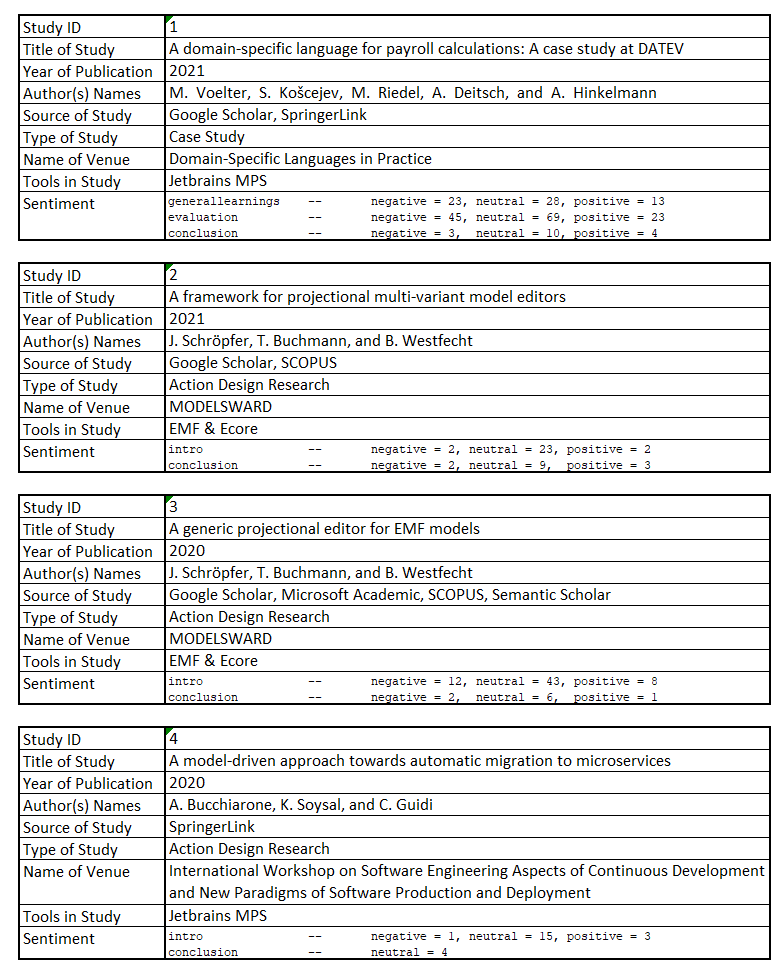
\includegraphics[width=0.85\textwidth]{Appendices/images/SLR_cards_1_to_4.png}}
    \caption{Data extraction results 1 - 4}
    \label{fig:DataExtraction_1_to_4}
\end{figure}
 
\begin{figure}
    \centering
    \fbox{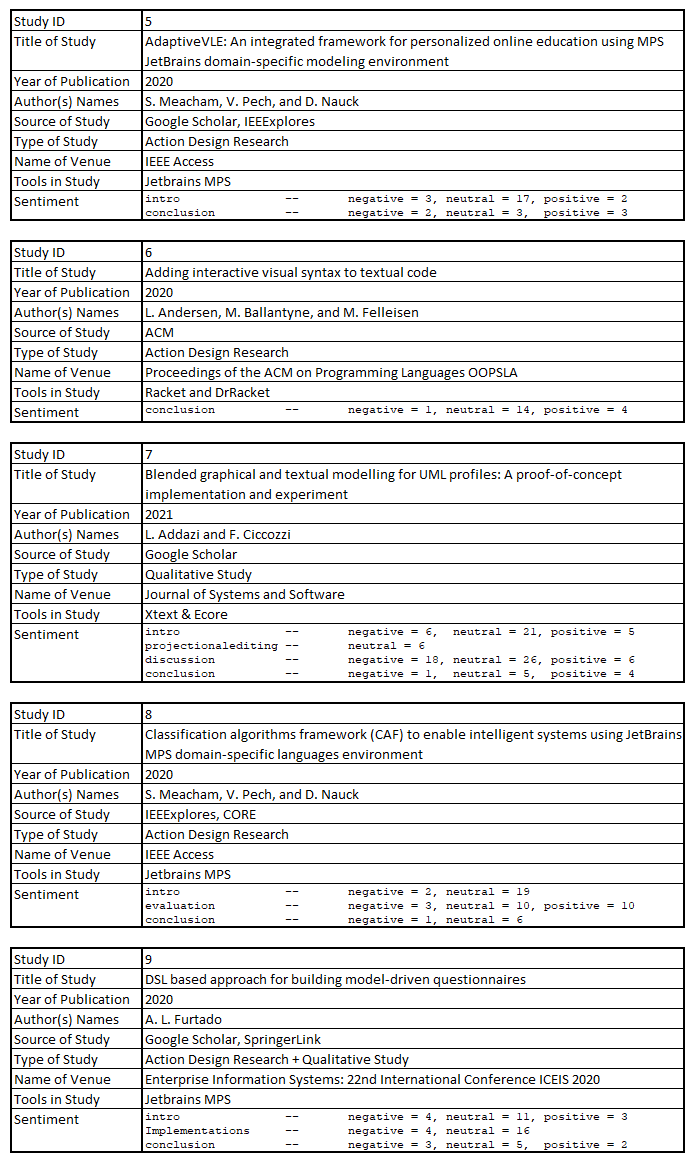
\includegraphics[width=0.90\textwidth]{Appendices/images/SLR_cards_5_to_9.png}}
    \caption{Data extraction results 5 - 9}
    \label{fig:DataExtraction_5_to_9}
\end{figure}
 
\begin{figure}
    \centering
    \fbox{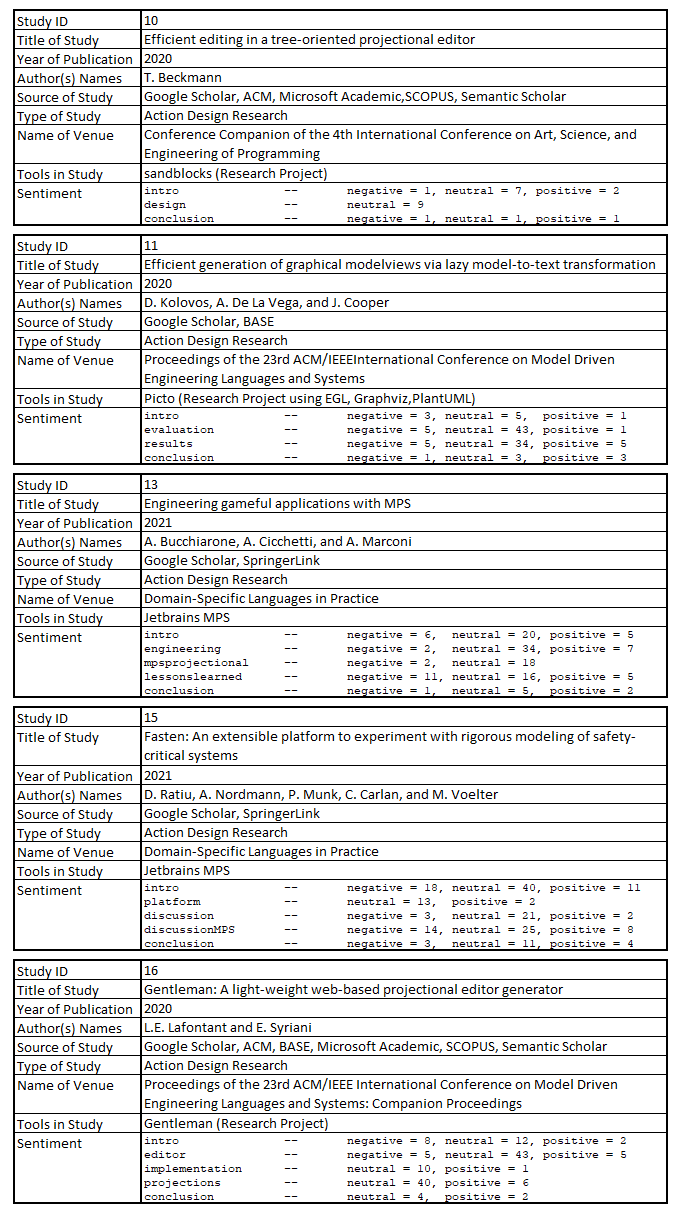
\includegraphics[width=0.87\textwidth]{Appendices/images/SLR_cards_10_to_16.png}}
    \caption{Data extraction results 10 - 16}
    \label{fig:DataExtraction_10_to_16}
\end{figure}
 
\begin{figure}
    \centering
    \fbox{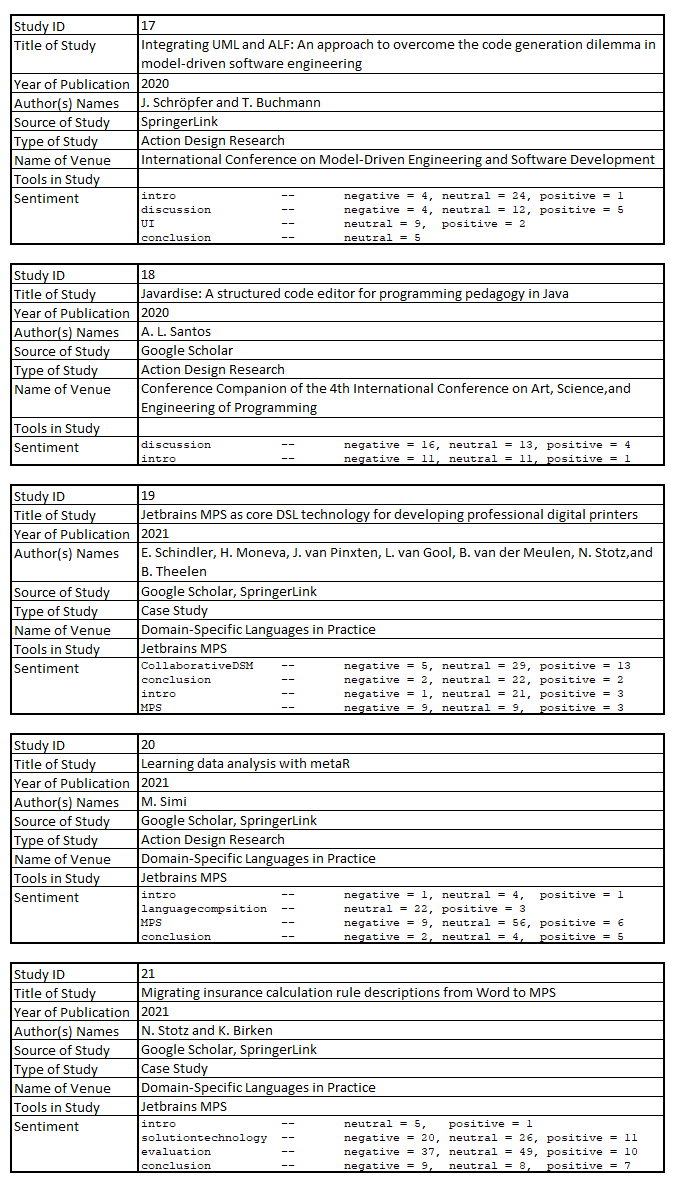
\includegraphics[width=0.87\textwidth]{Appendices/images/SLR_cards_17_to_21.png}}
    \caption{Data extraction results 17 - 21}
    \label{fig:DataExtraction_17_to_21}
\end{figure}
 
\begin{figure}
    \centering
    \fbox{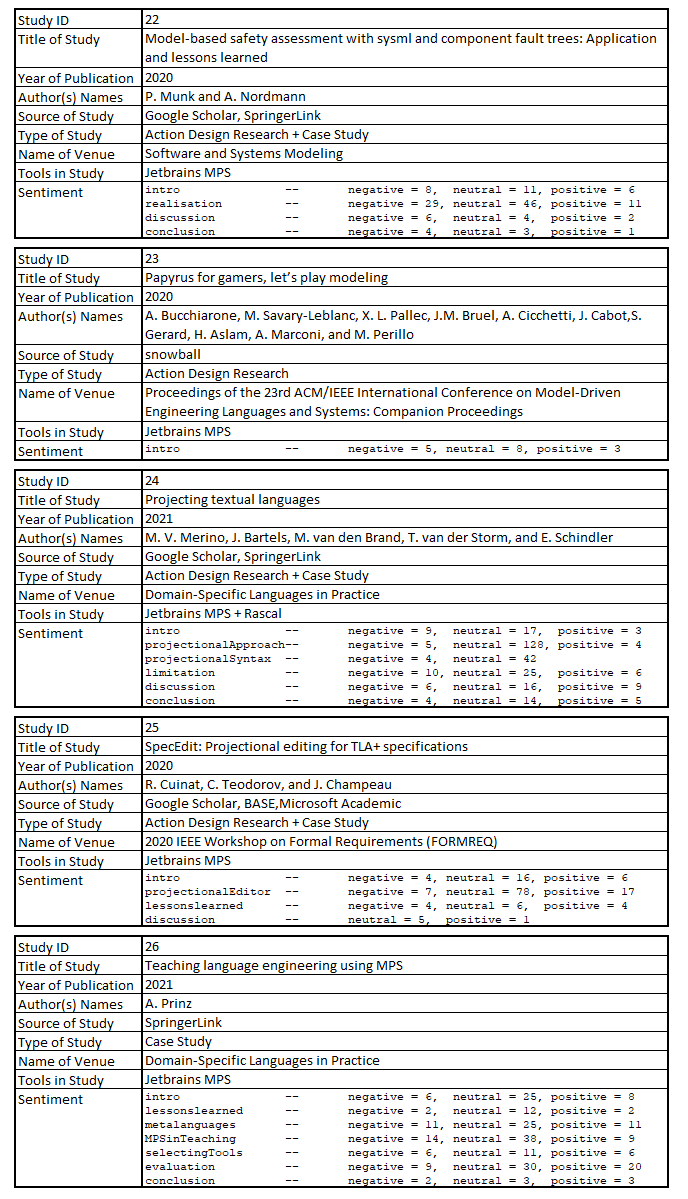
\includegraphics[width=0.87\textwidth]{Appendices/images/SLR_cards_22_to_26.png}}
    \caption{Data extraction results 22 - 26}
    \label{fig:DataExtraction_22_to_26}
\end{figure}
 
\begin{figure}
    \centering
    \fbox{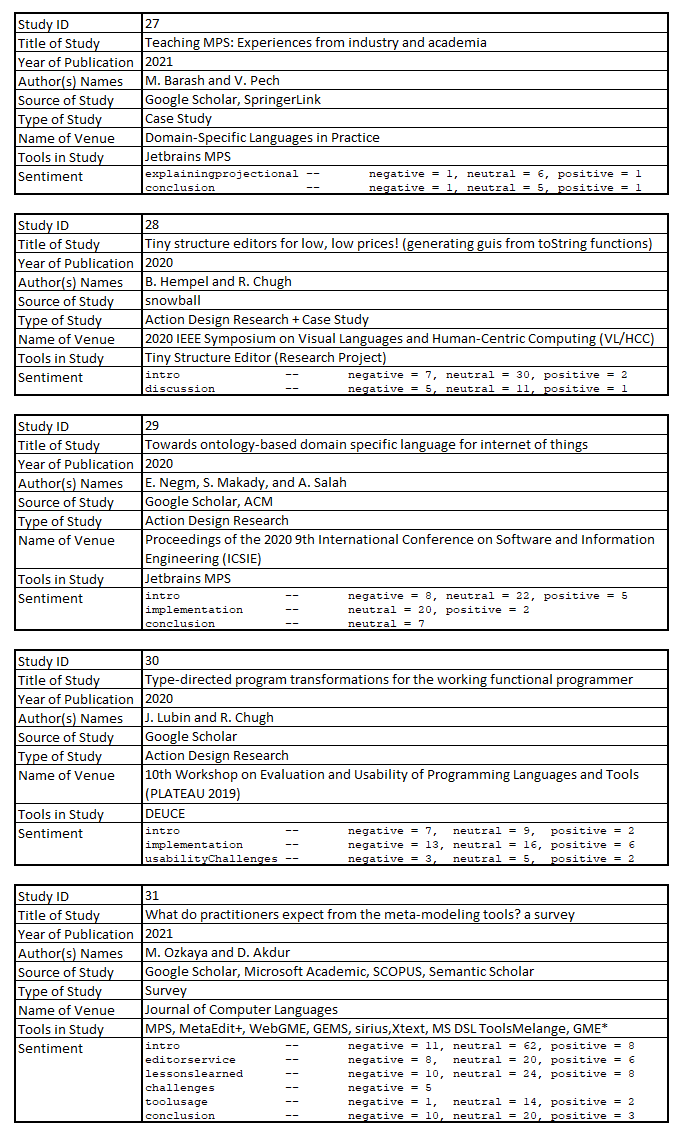
\includegraphics[width=0.90\textwidth]{Appendices/images/SLR_cards_27_to_31.png}}
    \caption{Data extraction results 27 - 31}
    \label{fig:DataExtraction_27_to_31}
\end{figure}
    \chapter{Drools Concept hierarchy}
\label{appendix:DroolsConceptHierarchy}

The concept hierarchy presented on the following pages was extracted and interpreted from Drools railroad diagrams.

The diagram in figure \ref{fig:RuleFileDiagram} represents the file level and can be considered the root of Concept Hierarchy.
This represents the concepts that are available to the rule file.
As the only concept we will examine in depth is the rule, we show some concepts that are shared or are children of, for example, function, query and type declaration.

In our final implementation only the import, global and Rule concepts that were children of the rule file were implemented.

The diagram in figure \ref{fig:RuleDiagram} shows the children of a rule.
Each attribute has a different behavior and structure and are thus all represented separately.

In These diagrams we do not show a concept diagram for the RHS.
This is because it would be more or less the concept diagram for Java Statements,with the addition of Rule Variables and some special Drools functions.
the concept diagram for a General Purpose Language, like Java, would be orders of magnitude bigger and more complex.
Luckily, as MPS allows for almost seamless extension and integration of different languages, we are able to just import JetBrains implementation of Java for the RHS.

The hierarch for the LHS is shown in the diagram in figure \ref{fig:LHSDiagram}.
Because of the number of concepts being represented, it may be a little hard to read.

\begin{figure}[h]
    \centering
    \fbox{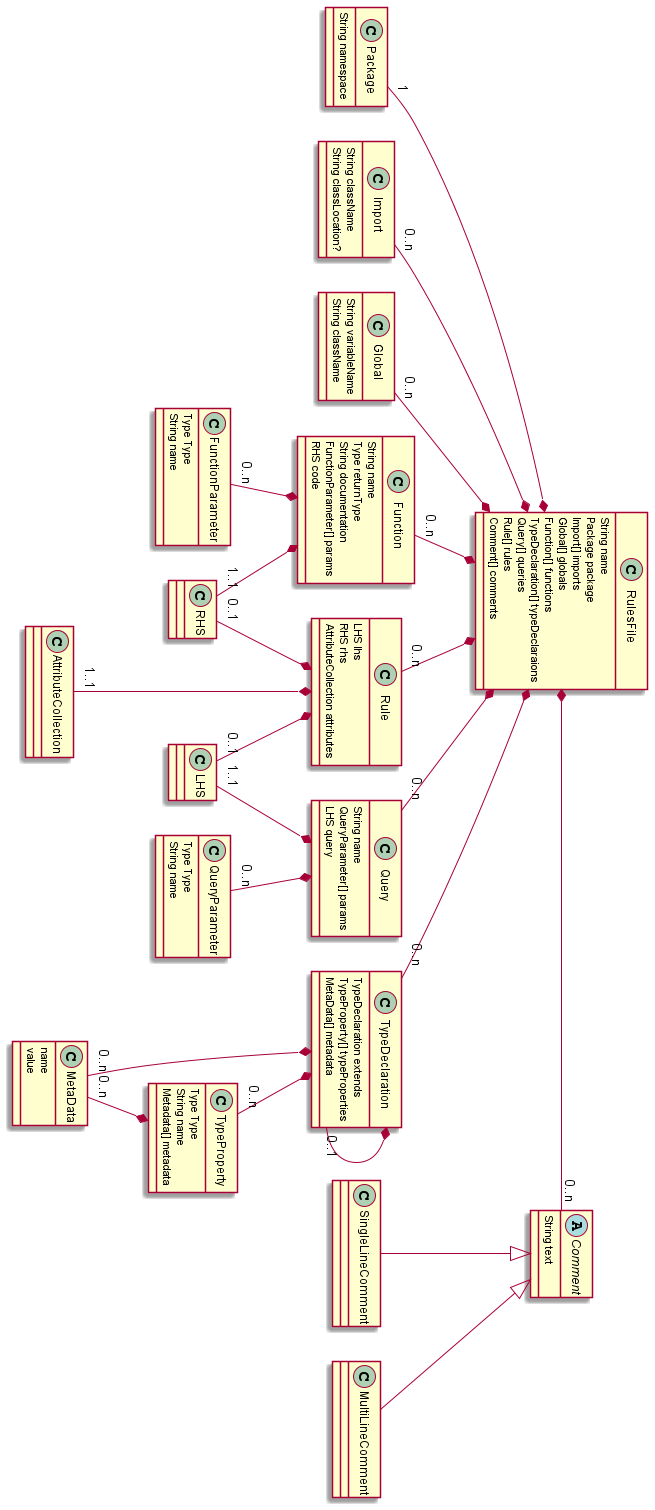
\includegraphics[width=0.75\textwidth]{Appendices/images/Droolsstructurerulefile.png}}
    \caption{Rule File Concept Hierarchy Diagram}
    \label{fig:RuleFileDiagram}
\end{figure}
 

\begin{figure}[h]
    \centering
    \fbox{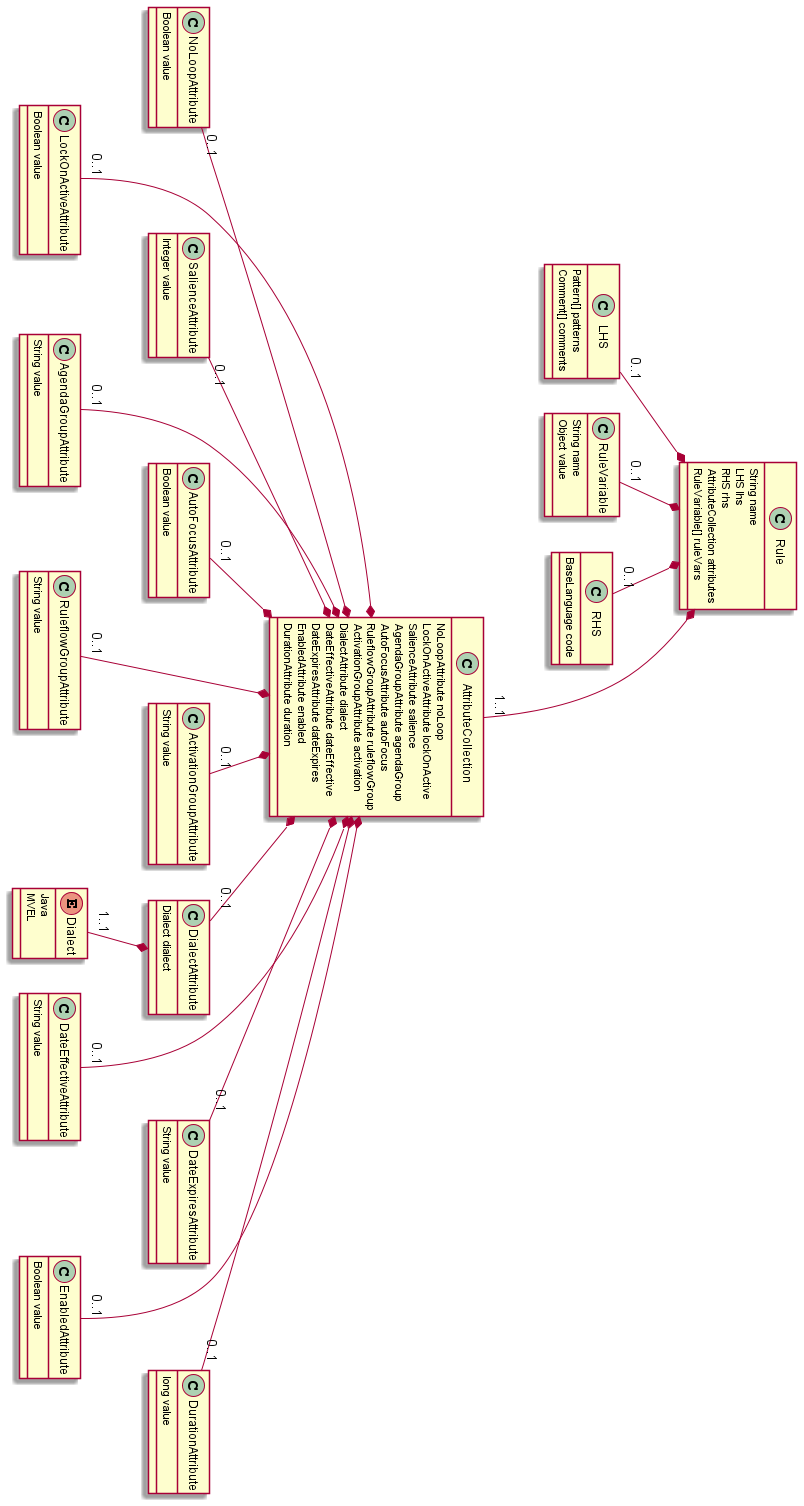
\includegraphics[width=0.95\textwidth]{Appendices/images/Droolsstructurerules.png}}
    \caption{Rules Concept Hierarchy Diagram}
    \label{fig:RuleDiagram}
\end{figure}
 

\begin{figure}[h]
    \centering
    \fbox{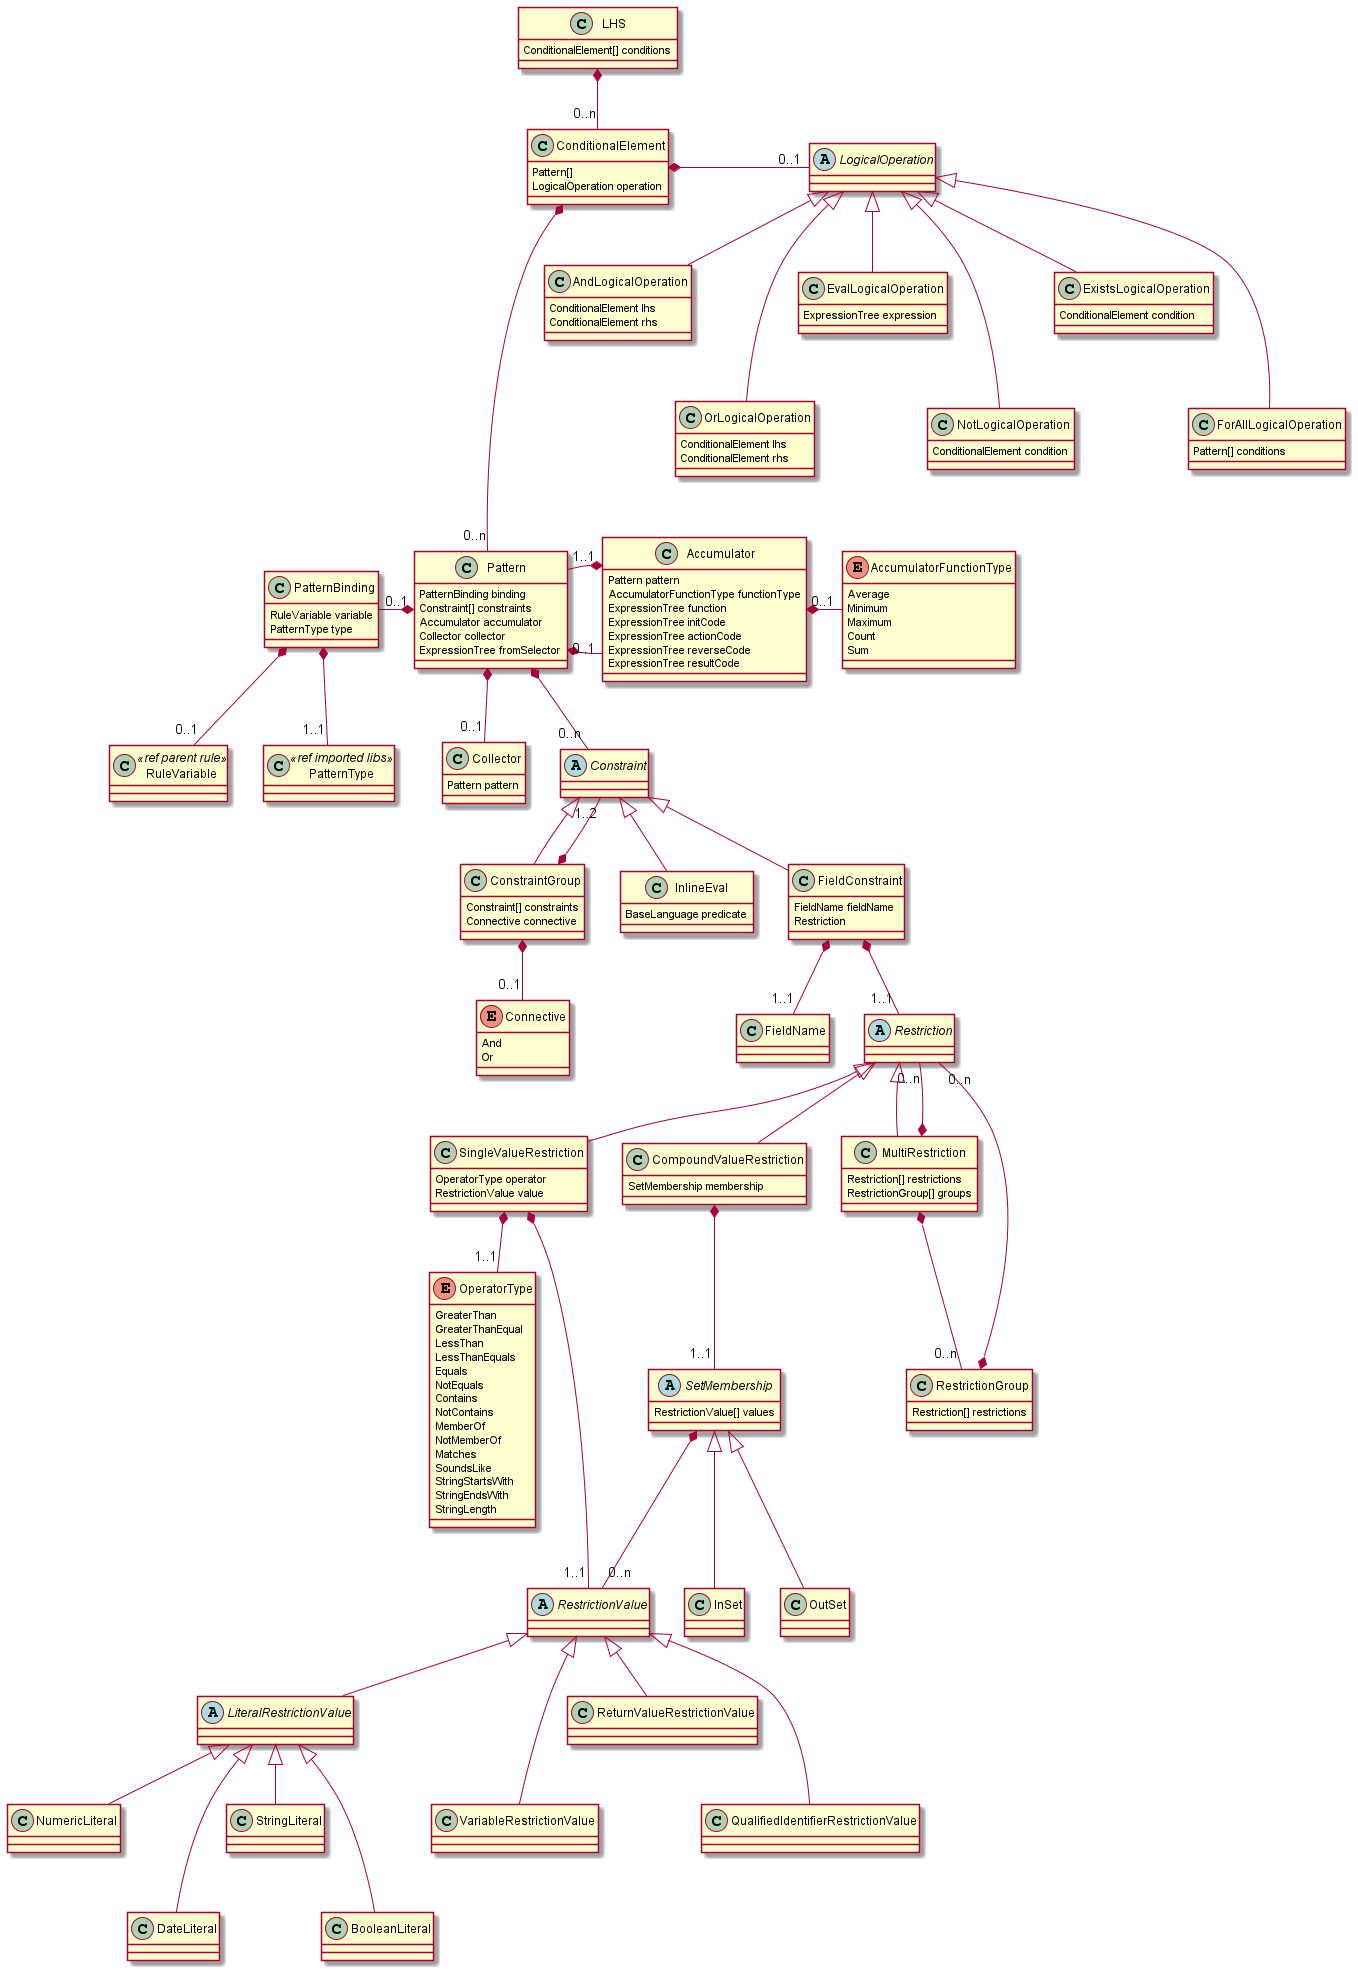
\includegraphics[width=0.99\textwidth]{Appendices/images/DroolsStructureLHS.png}}
    \caption{Rule LHS Concept Hierarchy Diagram}
    \label{fig:LHSDiagram}
\end{figure}
 
    \chapter{Questionnaire Text}
\label{Appendix:Questionaire_text}

Note: This questionnaire was presented on Survey Monkey and thus the text here is a best approximation of their paging system.


\section*{Page 1 - Introduction}

Thank you for taking part in this research.

According to Survey Monkey, this survey should take 6 minutes to complete, when we tested it, the average was closer to 10 minutes.

This survey is for the validation section of a research master's project by Paul Spencer at the University of Amsterdam.

The purpose is to determine whether projectional editing can be used to aid the comprehensibility of business rules.

We are using Drools as our example business rules language.

You were selected as you asked or answered a Drools question on StackOverflow, listed Drools as a skill on your LinkedIn profile, or were referred to this survey by someone who previously answered this survey.
(please feel free to forward this survey to anyone you know with Drools experience).

It is therefore assumed you are aware of what Drools is.

Projectional editing is a form of writing computer programs directly rather than writing text and having that parsed to create the program.
This allows the developer multiple views and editors for the same code.

In this survey, we will present you with a few of these views.

On the following page, there is an animated GIF that will give a small demonstration of what this means.

Figure \ref{fig:questionnaire_intro} shows how this is presented to the subject.

\section*{Page 2 - Example of Projectional editing in Drools}

Below is an animated GIF showing an example of a projectional implementation of Drools.

The top section is a tabular projection of the program.

The bottom part is a textual projection of the same program shown at the same time.

In this recording, we are editing in the tabular projection, which automatically updates the textual projection.

\emph{\underline{Here is placed an animated GIF of a demonstration of our prototype}}

\textbf{Question}: What is your first reaction to this mode of code editing?

Options: Very positive, Somewhat positive, Neutral, Somewhat negative, Very negative 

\emph{\underline{the order of the options will be randomly presented as either ``Very positive'' to ``Very negative'' or ``Very negative'' to ``Very positive''}}

Figure \ref{fig:questionnaire_firstImpression} shows how this is presented to the subject.

\section*{Page 3 - Positive about projectional editing}

\emph{\underline{This page is only selected if the user chose very positive or somewhat positive}}

This question is optional.

you may use the Green ``PREV'' button to review the previous page.

\textbf{Question}: how would this coding style be useful to your interactions with Drools?

This is an open question with a text box.

Figure \ref{fig:questionnaire_positive} shows how this is presented to the subject.

\section*{Page 4 - negative about projections}

\emph{\underline{This page is only selected if the user chose very positive or somewhat positive}}

This question is optional.

you may use the Green ``PREV'' button to review the previous page.

\textbf{Question}: What do you find negative with this style of coding

This is an open question with a text box.

\section*{Page 5 - Testing a projection}
\emph{\underline{In questionnaire version A \& D page 5 will be Testing a projection}}

\emph{\underline{In questionnaire version B \& C page 5 will be Testing textual projection}}

On this page, we present you with an example projection of a collection of Drools rules, in this case, as a sort of decision table.

We will ask you to describe what you think it does, if you can't that is also good data for us.

A brief description of how this projection works follows:

\emph{\underline{for the decision table the following text:}}

1) each row is a rule

2) each column is a fact, or, when indented, a selection criteria of that fact

3) smiley faces indicate that a fact has been selected for a rule

4) if a fact has been selected and a variable is bound to it then the variable name appears instead of the smiley face.

5) the ``Then'' part of the rule appears in the ``Actions'' column

\emph{\underline{for the other table the following text:}}

1) each row is a rule

2) each column is for a variable or a property of a fact

3) if a property is selected then the selection criteria is in the appropriate cell

4) unselected cells are indicated by a grey/beige colour

5) the ``Then'' part of the rule appears in the ``Actions'' column


\emph{\underline{depending on the version of this questionnaire the respondent will see one of the following pictures}}

\emph{\underline{Version A - decision table showing rule set 1 (FNWI)}}

\emph{\underline{Version B - decision table showing rule set 2 (LAW)}}

\emph{\underline{Version C - new table showing rule set 1}}

\emph{\underline{Version D - new table showing rule set 2}}

\textbf{Question}: Please describe what you think this group of rules does

This is an open question with a text box.

\textbf{Question}: How easy or difficult was it to describe this rule set?

Options: Very easy, Somewhat easy, Neutral, Somewhat difficult, Very difficult 

\emph{\underline{the order of the options will be randomly presented as either ``Very easy'' to ``Very difficult'' or ``Very difficult'' to ``Very easy''}}

Figure \ref{fig:questionnaire_describeProjection} shows how this is presented to the subject.

\section*{Page 6 - Testing textual projection}
\emph{\underline{In questionnaire version A \& D page 6 will be Testing textual projection}}

\emph{\underline{In questionnaire version B \& C page 6 will be Testing a projection}}

Here we present you a textual projection of Drools rules.

[Note: These are not the same rules as on the previous page]

\emph{\underline{depending on the version of this questionnaire the respondent will see one of the following pictures}}

\emph{\underline{Version A \& C - a text projection of rule set 2 (LAW)}}

\emph{\underline{Version B \& D - a text projection of rule set 1 (FNWI)}}

\textbf{Question}: Please describe what you think this group of rules does

This is an open question with a text box.

\textbf{Question}: How easy or difficult was it to describe this rule set?

Options: Very easy, Somewhat easy, Neutral, Somewhat difficult, Very difficult 

\emph{\underline{the order of the options will be randomly presented as either ``Very easy'' to ``Very difficult'' or ``Very difficult'' to ``Very easy''}}

Figure \ref{fig:questionnaire_describeText} shows how this is presented to the subject.

\section*{Page 7 - Comparing projections 1}

In this question, we ask to compare a new projection to a previously shown projection, on the page named ``Testing a projection''.

If you wish to reacquaint yourself with the previous projection, you can use the Green ``PREV''  button at the bottom of this page.

A brief description of how this new projection works follows:

\emph{\underline{for the decision table the following text:}}

1) each row is a rule

2) each column is a fact, or, when indented, a selection criteria of that fact

3) smiley faces indicate that a fact has been selected for a rule

4) if a fact has been selected and a variable is bound to it then the variable name appears instead of the smiley face.

5) the ``Then'' part of the rule appears in the ``Actions'' column


\emph{\underline{for the other table the following text:}}

1) each row is a rule

2) each column is for a variable or a property of a fact

3) if a property is selected then the selection criteria is in the appropriate cell

4) unselected cells are indicated by a grey/beige colour

5) the ``Then'' part of the rule appears in the ``Actions'' column

\emph{\underline{depending on the version of this questionnaire the respondent will see one of the following pictures}}

\emph{\underline{Version A - new table showing rule set 1}}

\emph{\underline{Version B - new table showing rule set 2}}

\emph{\underline{Version C - decision table showing rule set 1}}

\emph{\underline{Version D - decision table showing rule set 2}}

\textbf{Question}: How does the above projection compare to the first projection you described?

Options: Much easier to understand, Somewhat easier to understand, Neutral, Somewhat harder to understand, Much harder to understand

\emph{\underline{the order of the options will be randomly presented as either ``Much easier to understand'' to ``Much harder to understand'' or ``Much harder to understand'' to ``Much easier to understand'' }}

Figure \ref{fig:questionnaire_compareProjections} shows how this is presented to the subject.

\section*{Page 8 - Comparing projections 2}

In this question, we again ask to compare the new projection, this time to the textual projection, on the page named ``Testing textual projection''.

If you wish to reacquaint yourself with the textual projection, you can, of course, use the Green ``PREV'' button at the bottom of this page again.

\emph{\underline{depending on the version of this questionnaire the respondent will see one of the following pictures}}

\emph{\underline{Version A - new table showing rule set 2}}

\emph{\underline{Version B - new table showing rule set 1}}

\emph{\underline{Version C - decision table showing rule set 2}}

\emph{\underline{Version D - decision table showing rule set 1}}

\textbf{Question}: How does the above projection compare to the text Drools rules you described?

Options: Much easier to understand, Somewhat easier to understand, Neutral, Somewhat harder to understand, Much harder to understand

\emph{\underline{the order of the options will be randomly presented as either ``Much easier to understand'' to ``Much harder to understand'' or ``Much harder to understand'' to ``Much easier to understand'' }}

Figure \ref{fig:questionnaire_compareWithText} shows how this is presented to the subject.

\section*{Page 9 - Single rule helper 1 - Truth table}
\emph{\underline{In questionnaire version A \& D page 9 will be the Truth Table}}

\emph{\underline{In questionnaire version B \& C page 9 will be the Circuit Diagram}}

Below we present another projection.
This is a truth table projection.
It highlights the conditions that have to be true for a rule to be selected.

The GIF shows the rule selected and the developer pressing the up and down arrow keys to step through the different true (highlighted in green)  and false (highlighted in red) fact selections that result in a true outcome.

\emph{\underline{An animated GIF of the truth table example}}

\textbf{Question}: Would this help you with understanding your Drools rules?

Options: It would really help understanding, it would somewhat help understanding, Neutral, It would add a little confusion, It would add a lot of confusion

\emph{\underline{the order of the options will be randomly presented as either ``It would really help understanding'' to ``It would add a lot of confusion'' or ``It would add a lot of confusion'' to ``It would really help understanding''}}

Figure \ref{fig:questionnaire_truthTable} shows how this is presented to the subject.

\section*{Page 10 - Single rule helper 2 - Circuit Diagram}
\emph{\underline{In questionnaire version A \& D page 10 will be the Circuit Diagram}}

\emph{\underline{In questionnaire version B \& C page 10 will be the Truth Table}}

This is a circuit diagram of the selection conditions.
choosing a different condition highlights how they are related to each other.

The GIF shows the rule selected and the developer pressing the up and down arrow keys to step through the different fact selections (highlighted in yellow) and shown in the circuit diagram, thus showing how the facts relate to each other.

\emph{\underline{An animated GIF of the Circuit Diagram example}}

\textbf{Question}: Would this help you with understanding your Drools rules?

Options: It would really help understanding, it would somewhat help understanding, Neutral, It would add a little confusion, It would add a lot of confusion

\emph{\underline{the order of the options will be randomly presented as either ``It would really help understanding'' to ``It would add a lot of confusion'' or ``It would add a lot of confusion'' to ``It would really help understanding''}}

Figure \ref{fig:questionnaire_circuitDiagram} shows how this is presented to the subject.

\section*{Page 11 - The Statistics page}
Here we ask for data that we can use to slice and dice results.

\textbf{Question}: How long was/is your career as a developer?

Options: 0-1 year, 1-3 years, 3-10 years, greater than 10 years, none of the above

\textbf{Question}: When was the last time you had a coding interaction with Drools?

Options: during this week, some time after July 1st 2021, some time after Jan 1st 2021, some time after 2016, some time before 2016

\textbf{Question}: how long did you work with Drools?

Options: for years and intensely, for years but occasionally, not for long but intensely, I barely touched it


\textbf{Question}: Which tools have you used to edit Drools rules?

Checkboxes: Drools workbench, eclipse (with Drools plug-in), IntelliJ IDEA (with Drools plug-in), IDE or text editor without Drools assistance, other (please specify) \emph{\underline{has textbox}}, none of the above

Figure \ref{fig:questionnaire_personalDetails} shows how this is presented to the subject.

\section*{Page 12 - So long, and thanks for all the fish}
Thank you for your time.
We leave you with a box where you can put in any thoughts about this if you feel like it.

\textbf{Question}: Do you have any thoughts or opinions you would like to share about what you have seen in this questionnaire?

This is an open question with a text box.

Figure \ref{fig:questionnaire_comments} shows how this is presented to the subject.

\begin{figure}
    \centering
    \fbox{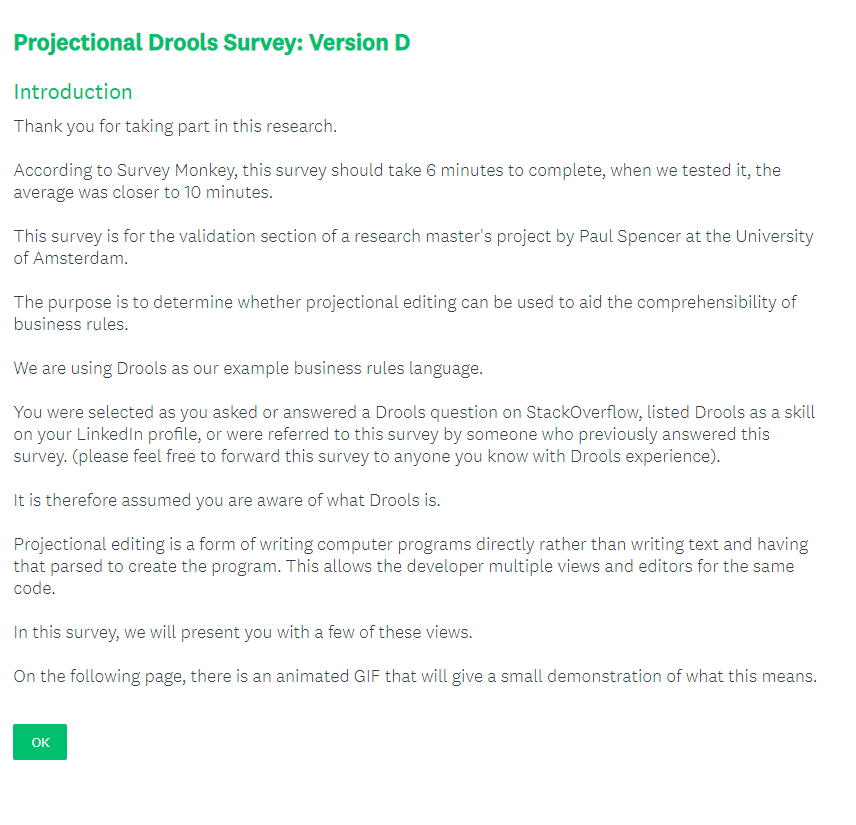
\includegraphics[width=0.95\textwidth]{Appendices/images/questionnaire_1.png}}
    \caption{Screen 1 - introduction text}
    \label{fig:questionnaire_intro}
\end{figure}
 
\begin{figure}
    \centering
    \fbox{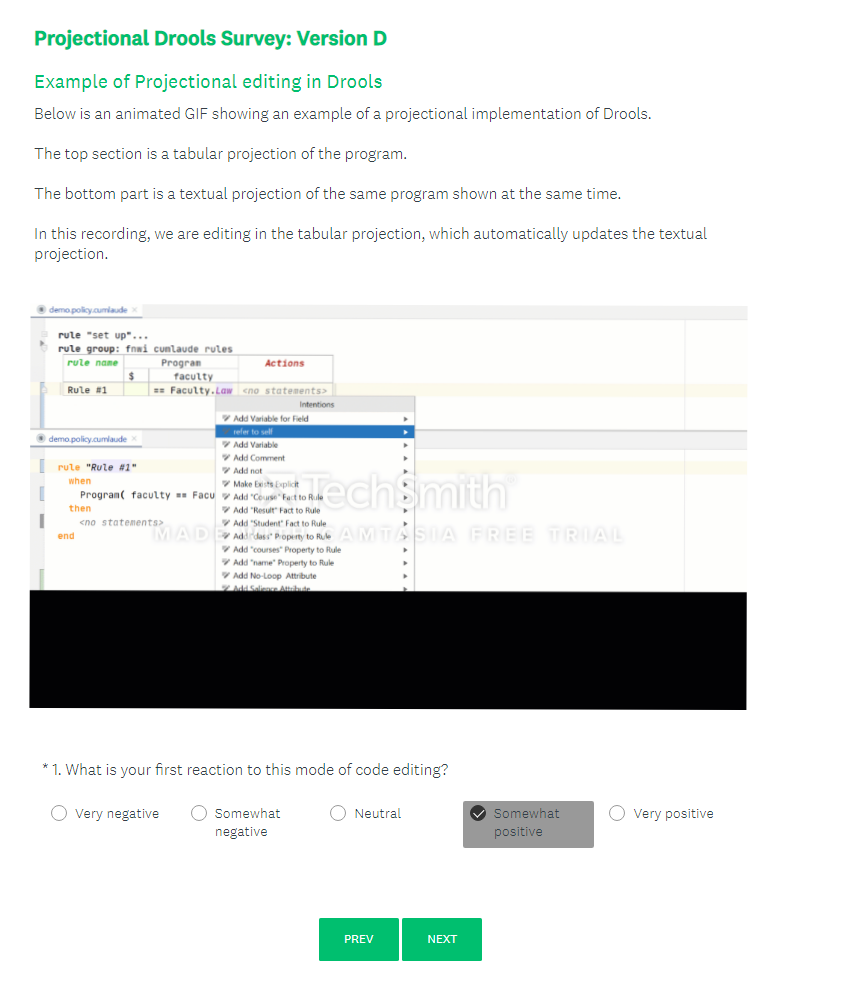
\includegraphics[width=0.95\textwidth]{Appendices/images/questionnaire_2.png}}
    \caption{Screen 2 - first impression}
    \label{fig:questionnaire_firstImpression}
\end{figure}
 
\begin{figure}
    \centering
    \fbox{\includegraphics[width=0.95\textwidth]{Appendices/images/questionnaire_3.png}}
    \caption{Screen 3 - positive response}
    \label{fig:questionnaire_positive}
\end{figure}
 
\begin{figure}
    \centering
    \fbox{\includegraphics[width=0.95\textwidth]{Appendices/images/questionnaire_4.png}}
    \caption{Screen 4 - describe projection}
    \label{fig:questionnaire_describeProjection}
\end{figure}
 
\begin{figure}
    \centering
    \fbox{\includegraphics[width=0.95\textwidth]{Appendices/images/questionnaire_5.png}}
    \caption{Screen 5 - describe text}
    \label{fig:questionnaire_describeText}
\end{figure}
 
\begin{figure}
    \centering
    \fbox{\includegraphics[width=0.95\textwidth]{Appendices/images/questionnaire_6.png}}
    \caption{Screen 6 - compare projections}
    \label{fig:questionnaire_compareProjections}
\end{figure}
 
\begin{figure}
    \centering
    \fbox{\includegraphics[width=0.95\textwidth]{Appendices/images/questionnaire_7.png}}
    \caption{Screen 7 - compare projection to text}
    \label{fig:questionnaire_compareWithText}
\end{figure}
 
\begin{figure}
    \centering
    \fbox{\includegraphics[width=0.95\textwidth]{Appendices/images/questionnaire_8.png}}
    \caption{Screen 8 - truth table}
    \label{fig:questionnaire_truthTable}
\end{figure}
  
\begin{figure}
    \centering
    \fbox{\includegraphics[width=0.95\textwidth]{Appendices/images/questionnaire_9.png}}
    \caption{Screen 9 - circuit diagram}
    \label{fig:questionnaire_circuitDiagram}
\end{figure}
   
\begin{figure}
    \centering
    \fbox{\includegraphics[width=0.95\textwidth]{Appendices/images/questionnaire_10.png}}
    \caption{Screen 10 - personal details page}
    \label{fig:questionnaire_personalDetails}
\end{figure}
   
\begin{figure}
    \centering
    \fbox{\includegraphics[width=0.95\textwidth]{Appendices/images/questionnaire_11.png}}
    \caption{Screen 11 - further comments}
    \label{fig:questionnaire_comments}
\end{figure}
\end{document} 
